% Options for packages loaded elsewhere
\PassOptionsToPackage{unicode}{hyperref}
\PassOptionsToPackage{hyphens}{url}
\PassOptionsToPackage{dvipsnames,svgnames,x11names}{xcolor}
%
\documentclass[
  letterpaper,
  DIV=11,
  numbers=noendperiod]{scrartcl}

\usepackage{amsmath,amssymb}
\usepackage{setspace}
\usepackage{iftex}
\ifPDFTeX
  \usepackage[T1]{fontenc}
  \usepackage[utf8]{inputenc}
  \usepackage{textcomp} % provide euro and other symbols
\else % if luatex or xetex
  \usepackage{unicode-math}
  \defaultfontfeatures{Scale=MatchLowercase}
  \defaultfontfeatures[\rmfamily]{Ligatures=TeX,Scale=1}
\fi
\usepackage{lmodern}
\ifPDFTeX\else  
    % xetex/luatex font selection
\fi
% Use upquote if available, for straight quotes in verbatim environments
\IfFileExists{upquote.sty}{\usepackage{upquote}}{}
\IfFileExists{microtype.sty}{% use microtype if available
  \usepackage[]{microtype}
  \UseMicrotypeSet[protrusion]{basicmath} % disable protrusion for tt fonts
}{}
\usepackage{xcolor}
\setlength{\emergencystretch}{3em} % prevent overfull lines
\setcounter{secnumdepth}{5}
% Make \paragraph and \subparagraph free-standing
\ifx\paragraph\undefined\else
  \let\oldparagraph\paragraph
  \renewcommand{\paragraph}[1]{\oldparagraph{#1}\mbox{}}
\fi
\ifx\subparagraph\undefined\else
  \let\oldsubparagraph\subparagraph
  \renewcommand{\subparagraph}[1]{\oldsubparagraph{#1}\mbox{}}
\fi


\providecommand{\tightlist}{%
  \setlength{\itemsep}{0pt}\setlength{\parskip}{0pt}}\usepackage{longtable,booktabs,array}
\usepackage{calc} % for calculating minipage widths
% Correct order of tables after \paragraph or \subparagraph
\usepackage{etoolbox}
\makeatletter
\patchcmd\longtable{\par}{\if@noskipsec\mbox{}\fi\par}{}{}
\makeatother
% Allow footnotes in longtable head/foot
\IfFileExists{footnotehyper.sty}{\usepackage{footnotehyper}}{\usepackage{footnote}}
\makesavenoteenv{longtable}
\usepackage{graphicx}
\makeatletter
\def\maxwidth{\ifdim\Gin@nat@width>\linewidth\linewidth\else\Gin@nat@width\fi}
\def\maxheight{\ifdim\Gin@nat@height>\textheight\textheight\else\Gin@nat@height\fi}
\makeatother
% Scale images if necessary, so that they will not overflow the page
% margins by default, and it is still possible to overwrite the defaults
% using explicit options in \includegraphics[width, height, ...]{}
\setkeys{Gin}{width=\maxwidth,height=\maxheight,keepaspectratio}
% Set default figure placement to htbp
\makeatletter
\def\fps@figure{htbp}
\makeatother

\usepackage{fontspec}
\usepackage{multirow}
\usepackage{multicol}
\usepackage{colortbl}
\usepackage{hhline}
\newlength\Oldarrayrulewidth
\newlength\Oldtabcolsep
\usepackage{longtable}
\usepackage{array}
\usepackage{hyperref}
\usepackage{float}
\usepackage{wrapfig}
% \usepackage{hyperref}
% \hypersetup{
%     colorlinks,
%     linkcolor={blue!100!black},
%     citecolor={blue!100!black},
%     urlcolor={blue!100!black}
% }
% \usepackage{apacite}
% \usepackage[round]{natbib} 
% \usepackage{graphicx}
% \usepackage{float}
% \usepackage{caption}
% \usepackage[toc,page]{appendix}
% \usepackage{booktabs,caption}
% \usepackage[flushleft]{threeparttable}
% \usepackage{tabularx}
\usepackage{sfmath}
\usepackage{fontspec}
\usepackage[utf8]{inputenc}
\usepackage{siunitx}
\usepackage{amsfonts}
\usepackage{amsmath}
% \usepackage{xcolor}
% \usepackage{scrextend}
% \deffootnote[2em]{2em}{1em}{\textsuperscript{\thefootnotemark}\,}
% \newcolumntype{Y}{>{\centering\arraybackslash}X}
% \usepackage[a4paper]{geometry}
% \usepackage{caption}
% \usepackage[bottom,flushmargin,hang,multiple]{footmisc}
% \usepackage{pdflscape}
% \usepackage[paper=portrait,pagesize]{typearea}
% \usepackage{rotating}
% \usepackage{fullpage}
% \usepackage{tabu}
\usepackage{lscape}
\newcommand{\blandscape}{\begin{landscape}}
\newcommand{\elandscape}{\end{landscape}}
\usepackage{rotating}
\newcommand{\bsideways}{\begin{sidewaystable}}
\newcommand{\esideways}{\end{sidewaystable}}
\KOMAoption{captions}{tableheading}
\makeatletter
\makeatother
\makeatletter
\makeatother
\makeatletter
\@ifpackageloaded{caption}{}{\usepackage{caption}}
\AtBeginDocument{%
\ifdefined\contentsname
  \renewcommand*\contentsname{Table of contents}
\else
  \newcommand\contentsname{Table of contents}
\fi
\ifdefined\listfigurename
  \renewcommand*\listfigurename{List of Figures}
\else
  \newcommand\listfigurename{List of Figures}
\fi
\ifdefined\listtablename
  \renewcommand*\listtablename{List of Tables}
\else
  \newcommand\listtablename{List of Tables}
\fi
\ifdefined\figurename
  \renewcommand*\figurename{Figure}
\else
  \newcommand\figurename{Figure}
\fi
\ifdefined\tablename
  \renewcommand*\tablename{Table}
\else
  \newcommand\tablename{Table}
\fi
}
\@ifpackageloaded{float}{}{\usepackage{float}}
\floatstyle{ruled}
\@ifundefined{c@chapter}{\newfloat{codelisting}{h}{lop}}{\newfloat{codelisting}{h}{lop}[chapter]}
\floatname{codelisting}{Listing}
\newcommand*\listoflistings{\listof{codelisting}{List of Listings}}
\makeatother
\makeatletter
\@ifpackageloaded{caption}{}{\usepackage{caption}}
\@ifpackageloaded{subcaption}{}{\usepackage{subcaption}}
\makeatother
\makeatletter
\@ifpackageloaded{tcolorbox}{}{\usepackage[skins,breakable]{tcolorbox}}
\makeatother
\makeatletter
\@ifundefined{shadecolor}{\definecolor{shadecolor}{rgb}{.97, .97, .97}}
\makeatother
\makeatletter
\makeatother
\makeatletter
\makeatother
\ifLuaTeX
  \usepackage{selnolig}  % disable illegal ligatures
\fi
\usepackage[round]{natbib}
\bibliographystyle{apalike}
\IfFileExists{bookmark.sty}{\usepackage{bookmark}}{\usepackage{hyperref}}
\IfFileExists{xurl.sty}{\usepackage{xurl}}{} % add URL line breaks if available
\urlstyle{same} % disable monospaced font for URLs
\hypersetup{
  colorlinks=true,
  linkcolor={blue!000!black},
  filecolor={Maroon},
  citecolor={blue!000!black},
  urlcolor={blue!000!black},
  pdfcreator={LaTeX via pandoc}}

\author{}
\date{}

\begin{document}
\title{UP Paper}


% \author {Xolani Sibande\footnote{Ecconomic Research Department, South African Reserve Bank. Department of Economics, University of Pretoria, Pretoria, South Africa; Email: xolaniss@gmail.com.} \,\,}

\date{\today}
\maketitle

\begin{abstract}


\end{abstract}

\noindent\textbf{Keywords}:    \\
\textbf{JEL Codes}: 
\newpage

\ifdefined\Shaded\renewenvironment{Shaded}{\begin{tcolorbox}[boxrule=0pt, interior hidden, frame hidden, enhanced, borderline west={3pt}{0pt}{shadecolor}, sharp corners, breakable]}{\end{tcolorbox}}\fi

\setstretch{1.5}
\hypertarget{introduction}{%
\section{Introduction}\label{introduction}}

\textit{The pursuit for financial stability through macro-prudential policies could potentially imply financial exclusion, particularly in emerging countries such as South Africa. For instance, economic growth and development could be promoted through increased lending to small and medium businesses, who are riskier to lend to. However, macro-prudential policies are by nature aimed at reducing risks associated with lending. Therefore, a natural question that arises is whether macro-prudential policy is a constraint to or consistent with financial inclusion or greater banking competition?}

\hypertarget{literature-review}{%
\section{Literature Review}\label{literature-review}}

Our paper encompasses and contributes to various strands of literature.
It firstly encompasses literature on the response of banks to
macroprudential reforms and secondly, the response of banks to external
efforts aimed at enabling financial inclusion. The construction of
narrative macroprudential reforms and narrative accounts of financial
inclusion encompass literature on narrative methods of identification.

The objective(s) of macroprudential reforms are well documented and
continue to expand with further reforms being introduced to create
resilient banking
systems\footnote{See \cite{kashyap2004cyclical}, \cite{basel06}, \cite{cohen2016banks} and \cite{cerutti2018changes} among others.}.
The ongoing debate regarding the implications of the reforms,
particularly on lending behaviour of banks provide further insight on
the costs and benefits of making banking systems resilient through the
reforms.

Evidently, work on the cost or unintended consequences of
macroprudential reforms have dominated the debate.
\cite{noss2016estimating} highlight that tightened macroprudential
capital requirements can cause banks' cost of funding to rise and in
turn, prompt banks to pass the increase in their cost of funding to
borrowers in the form of high interest on loans and/or reduction in
credit extended. \cite{deli2017real} show that higher capital
requirements would lead banks to reduce their risk-weighted assets,
implying a downward shift in lending in order to meet the capital
requirements. As evidence, the former authors use a Vector
Autoregressive (VAR) model to estimate the effect of changes in banks'
capital requirements on lending in the United Kingdom (UK) and find that
tighter capital requirements are associated with a reduction in lending,
with the effect on corporate lending more pronounced relative to
household lending.

Earlier work by \cite{aiyar2016does} study the interaction of capital
requirements and monetary policy and response of UK banks to the two
policies. Their findings show that banks reduce lending in response to
tighter capital reforms and monetary policy. They also exploit the
heterogeneity of banks and find that large banks react to tighter
capital requirements only, while small banks react to both policies.
\cite{deli2017real} and \cite{mirzaei2022effectiveness} provide
cross-country evidence on the effect of macroprudential reforms. The
former authors conduct the analysis for banks in 125 countries and find
weak negative effects of capital stringency on loan growth, especially
for well-capitalized banks. \cite{mirzaei2022effectiveness} find similar
results for banks in 91 countries, where small, less-capitalized and
less-liquid banks reduce lending more in response to stringent capital
requirements relative to banks that are well-capitalized and
highly-liquid.

With the use of various Dynamic Stochastic General Equilibrium (DSGE)
models, \cite{angelini2015b} find that a one percentage point increase
in the capital ratio translates into a 0.09 percent loss in output
relative to the level that would have prevailed in the absence of
capital tightening. \cite{berka2018basel} study the interaction between
credit activity, Basel Accords banking regulations, household saving
decisions and project returns with the use of a DSGE model, calibrated
for the Canadian economy. They find that Basel Accords in the form of
capital requirements have an impact on loans, when project returns
decline throughout the cycle as the requirements prompt banks to ration
credit during downturns where project returns are low, implying
increased default risk by borrowers (entrepreneurs).

Interestingly, work on the potential effect of macroprudential reforms
in emerging markets is limited. The exception is recent work by
\cite{fang2022bank} who study the impact of rising capital requirements
on lending in Peru. They exploit bank-level lending data and
bank-specific capital buffers. Their findings show that higher capital
requirements are associated with lower credit extension. The effects
however vary according to economic conditions and bank characteristics,
where less capitalized, less liquid and less profitable banks react more
to tighter capital requirements. The effects are also more pronounced
during economic downturns. In the case of South Africa, earlier work by
\cite{maredza2016capital} investigates the impact of increased bank
requirements and in particular those introduced under Basel II on the
cost of intermediation. Results from a panel of ten banks show that
tighter capital requirements increase the cost of intermediation, with
the net interest margin serving as a proxy for the cost of
intermediation. \cite{gumata2017bank} assess the impact of Basel III in
the form of liquidity coverage ratio and net stable funding ratios on
credit growth. Their decomposition exercise shows that Basel III
contributed to the contraction in credit post the GFC.

Lastly, the construction of our narrative macroprudential reforms is
based on the literature documenting narrative methods of identification.
As outlined earlier, evidence on the response of bank lending to
macroprudential reforms is based on the assumption that an increase in
aggregate regulatory capital represents a negative credit supply shock
and in turn have a negative effect on credit extension
\citep{noss2016estimating}. As such, our narrative accounts of
macroprudential reforms implicitly proxy for credit supply shocks.
\cite{ramey2016macroeconomic} describes the narrative method of
identification as constructing a series from historical documents to
identify the reason and/or the quantities associated with a particular
change in a variable. Furthermore, the construction of narrative
accounts is particularly aimed at exclusively isolating shocks or
effects of policy intervention\citep{angelopoulou2007narrative}.
Therefore, by constructing a narrative series of macroprudential
reforms, we aim to address challenges relating to the identification of
macroprudential reforms and their impact thereof. The application of the
identification strategy has largely focused on identifying monetary and
fiscal
shocks\footnote{See \cite{romer1989does}, \cite{romer1997identification} \cite{romer2004new} \cite{romer2010macroeconomic} \cite{ramey2011identifying} ]\cite{ramey2016macroeconomic} \cite{ramey2018government}.}.
However, the approach is increasingly being applied to analyse and
identify capital reforms. For instance, \cite{budnik2020identifying}
analyse the dynamic effects of U.S macroprudential policies by
constructing a set of policy measures related to capital requirements
following the Basel III Accords. The narrative instruments take a value
of -1 and 1 in the case of tightening and easing of capital
requirements, respectively and 0 otherwise. Importantly, results from
their analysis show that tightening of capital requirements induces a
persistent decline in corporate credit. Further, the impact of a change
in capital requirements is concentrated more on corporate credit
relative to household credit. \cite{eickmeier2018macroeconomic} also
assess the dynamic effects of bank capital regulation in the U.S, where
they use the narrative approach to construct an exogenous capital
regulation index that captures exogenous changes in bank capital
regulation. Their results also show persistent declines in corporate and
investment loans and real estate loans, following changes in the capital
regulation index.

We therefore add to the growing empirical literature examining; (1) the
response of banks to changes in macroprudential reforms; (2)
particularly in emerging markets and (3); applying narrative methods of
identification.

\hypertarget{macroprudential-reforms-narrative-indicators}{%
\section{Macroprudential reforms: Narrative
Indicators}\label{macroprudential-reforms-narrative-indicators}}

This section presents actions and events we use to construct a set of
macroprudential measures or indicators introduced following Basel II
Agreements and Accords. The indicators represent credit supply shocks,
following \cite{noss2016estimating} and \cite{deli2017real} among
others. The construction is based on historical documents containing
actions and events that lead to the implementation of macroprudential
regulations, from 2008 to 2019. We consult circulars issued by the SARB
to commercial banks in South Africa, annual reports of commercial banks
and SARB and risk and capital management reports of commercial banks. We
consider reports of only the big 4 commercial banks in South Africa as
they account for over 90 percent of banking industry
assets.\footnote{The big 4 banks include Standard Bank, ABSA, NEDBANK and First Rand.}
We also consider documents published and issued by the Basel Committee
on Bank Supervision (BCBS), containing communication between BCBS and
SARB relating to the implementation of Basel regulations.

Due to the wide variety of information contained in the documents, we
impose a criteria with which we use to identify actions and events that
are most important in the construction of our narrative indicators.
Since the set of macorprudential indicators proxy for credit shocks, the
criteria imposed is such that: (1) actions and events are specific in
their intentions and (2), actions and events might imply a change in
bank behaviour with respect to the adjustment of capital buffers and/or
the attachment of greater risk weights to certain lending products or
lending markets. From this, we are able to build a series of two
narrative indicators \(z_{t}\) defined such that \(z_{t}=1\) for dates
of events containing announcements and communication of regulation
intended to be passed and the drafting of such regulation which we call
\(Draft\). The second indicator is such that \(z_{t}=1\) for dates of
events recording the eventual implementation of the regulation, which we
call \(Implementation\). For dates where \(Draft\) and
\(Implementation\) of regulation is not recorded \(z_{t}=0\). Therefore
where possible, we also track the actions and events from the date they
are communicated and or announced, issued or published (\(Draft\)),
until the date they are introduced or implemented (\(Implementation\)).

The decomposition of the actions and events is done with the aim of
possibly identifying anticipation effects following the drafting of
regulation not yet implemented. For instance,
\cite{eickmeier2018macroeconomic} analyse the macroeconomic effects of
bank capital requirement tightenings using a narrative index of bank
regulatory capital in the U.S. They find that bank assets (loans) and
industrial production fall 6 months before new rules become effective.
The anticipation effects are captured by the banks' actions between
dates when regulation is first mentioned in proposed rules and dates
when the final rule is communicated. In effect, anticipation effects are
therefore based on the notion that banks have information on the
proposed regulation and dates which they will be implemented and as
such, they can act (expand credit for instance) before implementation
date and thereby take advantage of less stringent requirements on credit
extension due to regulation before tighter requirements are introduced.

Information contained in the documents we use to construct our narrative
indicators also contain details enabling us to exploit such anticipation
effects.

Importantly, we do not identify the impact of individual regulations and
requirements under Basel Accords and Agreements but rather, we consider
Basel regulations in their entirety. Although different Basel
regulations such as the capital and liquidity requirements target
different instruments, the entirety of Basel regulations, which both
capital and liquidity requirements fall under, is aimed at creating
resilient and robust banking systems, through higher bank capital
requirements and subsequently, increased bank capital holdings
\citep{cohen2016banks} \citep{cerutti2018changes}.

As an example to some of the actions we use to construct the two sets of
indicators, the implementation of Basel II on January 1, 2008 is
categorized as an implementation indicator. Further example occurs on
February 4, 2009, which we categorize as a \(Draft\) indicator, where
the SARB issues directive 1/2009 (1 of 2009) announcing the approach
banks should follow in the application of capital floors. ``Modelled
capital should not be below 80\% of the capital requirements under Basel
I to ensure capital levels do not fall below prudent level''.

Following Basel II, banks are allowed to use internal models to
determine risk weights and in turn, determine capital levels. However,
capital floors ensure capital requirements did not fall below a certain
percentage of banks' capital requirements under the previous Basel I
framework\citep{basel06}. This in essence, imply greater risk weight
arched to riskier credit products. For instance,
\cite{imbierowicz2018time} show that Danish banks reducing their lending
on loans with higher risk weights, in response to higher capital
requirements, including approaches to capital floors. A further example
which is categorized as a \(Draft\) indicator and tracked until
implementation, occurs on July 31, 2009, where the BCBS announces
``measures to strengthen the 1996 rules governing trading book capital
and to enhance the three pillars of the Basel II framework (Basel
2.5)''. This in essence, aims to introduce higher capital requirements
to capture the credit risk of complex trading activities, promote the
build-up of capital buffers that can be drawn down in periods of stress
and strengthen the quality of bank capital\citep{basel09}. The SARB
endorsed and gave notices to banks to prepare for the implementation
therefore, on October 8, 2010, following the communication by the BCBS
on July 31, 2009. Following both communications and announcements, Basel
2.5 is eventually implemented January 1, 2012.

\hypertarget{data-and-methodology}{%
\section{Data and Methodology}\label{data-and-methodology}}

\hypertarget{data}{%
\subsection{Data}\label{data}}

Still to come\ldots{}
\textit{It is important to note that policy indicators capturing macroprudential reforms are not-bank specific . For instance, banks in our panel may at their discretion, increase their capital buffers in addition to minimum requirements. However, the minimum macroprudential (predominantly capital requirements) reforms are applied uniformly across banks}.

\newpage

\hypertarget{tbl-descriptive}{}
\global\setlength{\Oldarrayrulewidth}{\arrayrulewidth}

\global\setlength{\Oldtabcolsep}{\tabcolsep}

\setlength{\tabcolsep}{2pt}

\renewcommand*{\arraystretch}{0.5}



\providecommand{\ascline}[3]{\noalign{\global\arrayrulewidth #1}\arrayrulecolor[HTML]{#2}\cline{#3}}

\begin{longtable}[l]{|p{3.56in}|p{0.40in}|p{0.27in}|p{0.36in}|p{0.33in}|p{0.33in}|p{0.26in}}
\caption{\label{tbl-descriptive}Descriptive Statistics }\tabularnewline




\ascline{1pt}{000000}{1-7}

\multicolumn{1}{>{\raggedright}m{\dimexpr 3.56in+0\tabcolsep}}{\textcolor[HTML]{000000}{\fontsize{7}{7}\selectfont{Series}}} & \multicolumn{1}{>{\raggedleft}m{\dimexpr 0.4in+0\tabcolsep}}{\textcolor[HTML]{000000}{\fontsize{7}{7}\selectfont{Median}}} & \multicolumn{1}{>{\raggedleft}m{\dimexpr 0.27in+0\tabcolsep}}{\textcolor[HTML]{000000}{\fontsize{7}{7}\selectfont{SD}}} & \multicolumn{1}{>{\raggedleft}m{\dimexpr 0.36in+0\tabcolsep}}{\textcolor[HTML]{000000}{\fontsize{7}{7}\selectfont{Min}}} & \multicolumn{1}{>{\raggedleft}m{\dimexpr 0.33in+0\tabcolsep}}{\textcolor[HTML]{000000}{\fontsize{7}{7}\selectfont{Max}}} & \multicolumn{1}{>{\raggedleft}m{\dimexpr 0.33in+0\tabcolsep}}{\textcolor[HTML]{000000}{\fontsize{7}{7}\selectfont{IQR}}} & \multicolumn{1}{>{\raggedleft}m{\dimexpr 0.26in+0\tabcolsep}}{\textcolor[HTML]{000000}{\fontsize{7}{7}\selectfont{Obs}}} \\

\ascline{1pt}{000000}{1-7}\endfirsthead 

\ascline{1pt}{000000}{1-7}

\multicolumn{1}{>{\raggedright}m{\dimexpr 3.56in+0\tabcolsep}}{\textcolor[HTML]{000000}{\fontsize{7}{7}\selectfont{Series}}} & \multicolumn{1}{>{\raggedleft}m{\dimexpr 0.4in+0\tabcolsep}}{\textcolor[HTML]{000000}{\fontsize{7}{7}\selectfont{Median}}} & \multicolumn{1}{>{\raggedleft}m{\dimexpr 0.27in+0\tabcolsep}}{\textcolor[HTML]{000000}{\fontsize{7}{7}\selectfont{SD}}} & \multicolumn{1}{>{\raggedleft}m{\dimexpr 0.36in+0\tabcolsep}}{\textcolor[HTML]{000000}{\fontsize{7}{7}\selectfont{Min}}} & \multicolumn{1}{>{\raggedleft}m{\dimexpr 0.33in+0\tabcolsep}}{\textcolor[HTML]{000000}{\fontsize{7}{7}\selectfont{Max}}} & \multicolumn{1}{>{\raggedleft}m{\dimexpr 0.33in+0\tabcolsep}}{\textcolor[HTML]{000000}{\fontsize{7}{7}\selectfont{IQR}}} & \multicolumn{1}{>{\raggedleft}m{\dimexpr 0.26in+0\tabcolsep}}{\textcolor[HTML]{000000}{\fontsize{7}{7}\selectfont{Obs}}} \\

\ascline{1pt}{000000}{1-7}\endhead



\multicolumn{7}{>{\centering}m{\dimexpr 5.52in+12\tabcolsep}}{\textcolor[HTML]{000000}{\fontsize{7}{7}\selectfont{Lending\ growth}}} \\





\multicolumn{1}{>{\raggedright}m{\dimexpr 3.56in+0\tabcolsep}}{\textcolor[HTML]{000000}{\fontsize{7}{7}\selectfont{Three\ month\ change\ in\ log\ commercial\ mortgages\ to\ corporates\ and\ households}}} & \multicolumn{1}{>{\raggedleft}m{\dimexpr 0.4in+0\tabcolsep}}{\textcolor[HTML]{000000}{\fontsize{7}{7}\selectfont{1.16}}} & \multicolumn{1}{>{\raggedleft}m{\dimexpr 0.27in+0\tabcolsep}}{\textcolor[HTML]{000000}{\fontsize{7}{7}\selectfont{1.08}}} & \multicolumn{1}{>{\raggedleft}m{\dimexpr 0.36in+0\tabcolsep}}{\textcolor[HTML]{000000}{\fontsize{7}{7}\selectfont{-1.43}}} & \multicolumn{1}{>{\raggedleft}m{\dimexpr 0.33in+0\tabcolsep}}{\textcolor[HTML]{000000}{\fontsize{7}{7}\selectfont{3.81}}} & \multicolumn{1}{>{\raggedleft}m{\dimexpr 0.33in+0\tabcolsep}}{\textcolor[HTML]{000000}{\fontsize{7}{7}\selectfont{1.67}}} & \multicolumn{1}{>{\raggedleft}m{\dimexpr 0.26in+0\tabcolsep}}{\textcolor[HTML]{000000}{\fontsize{7}{7}\selectfont{153}}} \\





\multicolumn{1}{>{\raggedright}m{\dimexpr 3.56in+0\tabcolsep}}{\textcolor[HTML]{000000}{\fontsize{7}{7}\selectfont{Three\ month\ change\ in\ log\ household\ unsecured\ lending}}} & \multicolumn{1}{>{\raggedleft}m{\dimexpr 0.4in+0\tabcolsep}}{\textcolor[HTML]{000000}{\fontsize{7}{7}\selectfont{1.43}}} & \multicolumn{1}{>{\raggedleft}m{\dimexpr 0.27in+0\tabcolsep}}{\textcolor[HTML]{000000}{\fontsize{7}{7}\selectfont{2.49}}} & \multicolumn{1}{>{\raggedleft}m{\dimexpr 0.36in+0\tabcolsep}}{\textcolor[HTML]{000000}{\fontsize{7}{7}\selectfont{-10.40}}} & \multicolumn{1}{>{\raggedleft}m{\dimexpr 0.33in+0\tabcolsep}}{\textcolor[HTML]{000000}{\fontsize{7}{7}\selectfont{10.08}}} & \multicolumn{1}{>{\raggedleft}m{\dimexpr 0.33in+0\tabcolsep}}{\textcolor[HTML]{000000}{\fontsize{7}{7}\selectfont{1.78}}} & \multicolumn{1}{>{\raggedleft}m{\dimexpr 0.26in+0\tabcolsep}}{\textcolor[HTML]{000000}{\fontsize{7}{7}\selectfont{153}}} \\





\multicolumn{1}{>{\raggedright}m{\dimexpr 3.56in+0\tabcolsep}}{\textcolor[HTML]{000000}{\fontsize{7}{7}\selectfont{Three\ month\ change\ in\ log\ leasing\ and\ installments\ to\ corporates}}} & \multicolumn{1}{>{\raggedleft}m{\dimexpr 0.4in+0\tabcolsep}}{\textcolor[HTML]{000000}{\fontsize{7}{7}\selectfont{1.32}}} & \multicolumn{1}{>{\raggedleft}m{\dimexpr 0.27in+0\tabcolsep}}{\textcolor[HTML]{000000}{\fontsize{7}{7}\selectfont{1.48}}} & \multicolumn{1}{>{\raggedleft}m{\dimexpr 0.36in+0\tabcolsep}}{\textcolor[HTML]{000000}{\fontsize{7}{7}\selectfont{-1.69}}} & \multicolumn{1}{>{\raggedleft}m{\dimexpr 0.33in+0\tabcolsep}}{\textcolor[HTML]{000000}{\fontsize{7}{7}\selectfont{6.82}}} & \multicolumn{1}{>{\raggedleft}m{\dimexpr 0.33in+0\tabcolsep}}{\textcolor[HTML]{000000}{\fontsize{7}{7}\selectfont{2.04}}} & \multicolumn{1}{>{\raggedleft}m{\dimexpr 0.26in+0\tabcolsep}}{\textcolor[HTML]{000000}{\fontsize{7}{7}\selectfont{153}}} \\





\multicolumn{1}{>{\raggedright}m{\dimexpr 3.56in+0\tabcolsep}}{\textcolor[HTML]{000000}{\fontsize{7}{7}\selectfont{Three\ month\ change\ in\ log\ leasing\ and\ installments\ to\ households}}} & \multicolumn{1}{>{\raggedleft}m{\dimexpr 0.4in+0\tabcolsep}}{\textcolor[HTML]{000000}{\fontsize{7}{7}\selectfont{1.15}}} & \multicolumn{1}{>{\raggedleft}m{\dimexpr 0.27in+0\tabcolsep}}{\textcolor[HTML]{000000}{\fontsize{7}{7}\selectfont{1.29}}} & \multicolumn{1}{>{\raggedleft}m{\dimexpr 0.36in+0\tabcolsep}}{\textcolor[HTML]{000000}{\fontsize{7}{7}\selectfont{-2.56}}} & \multicolumn{1}{>{\raggedleft}m{\dimexpr 0.33in+0\tabcolsep}}{\textcolor[HTML]{000000}{\fontsize{7}{7}\selectfont{4.63}}} & \multicolumn{1}{>{\raggedleft}m{\dimexpr 0.33in+0\tabcolsep}}{\textcolor[HTML]{000000}{\fontsize{7}{7}\selectfont{1.54}}} & \multicolumn{1}{>{\raggedleft}m{\dimexpr 0.26in+0\tabcolsep}}{\textcolor[HTML]{000000}{\fontsize{7}{7}\selectfont{153}}} \\





\multicolumn{1}{>{\raggedright}m{\dimexpr 3.56in+0\tabcolsep}}{\textcolor[HTML]{000000}{\fontsize{7}{7}\selectfont{Three\ month\ change\ in\ log\ non-financial\ corporate\ unsecured\ lending}}} & \multicolumn{1}{>{\raggedleft}m{\dimexpr 0.4in+0\tabcolsep}}{\textcolor[HTML]{000000}{\fontsize{7}{7}\selectfont{1.54}}} & \multicolumn{1}{>{\raggedleft}m{\dimexpr 0.27in+0\tabcolsep}}{\textcolor[HTML]{000000}{\fontsize{7}{7}\selectfont{2.85}}} & \multicolumn{1}{>{\raggedleft}m{\dimexpr 0.36in+0\tabcolsep}}{\textcolor[HTML]{000000}{\fontsize{7}{7}\selectfont{-9.17}}} & \multicolumn{1}{>{\raggedleft}m{\dimexpr 0.33in+0\tabcolsep}}{\textcolor[HTML]{000000}{\fontsize{7}{7}\selectfont{8.04}}} & \multicolumn{1}{>{\raggedleft}m{\dimexpr 0.33in+0\tabcolsep}}{\textcolor[HTML]{000000}{\fontsize{7}{7}\selectfont{3.58}}} & \multicolumn{1}{>{\raggedleft}m{\dimexpr 0.26in+0\tabcolsep}}{\textcolor[HTML]{000000}{\fontsize{7}{7}\selectfont{153}}} \\





\multicolumn{1}{>{\raggedright}m{\dimexpr 3.56in+0\tabcolsep}}{\textcolor[HTML]{000000}{\fontsize{7}{7}\selectfont{Three\ month\ change\ in\ log\ residential\ mortgages\ to\ households}}} & \multicolumn{1}{>{\raggedleft}m{\dimexpr 0.4in+0\tabcolsep}}{\textcolor[HTML]{000000}{\fontsize{7}{7}\selectfont{0.77}}} & \multicolumn{1}{>{\raggedleft}m{\dimexpr 0.27in+0\tabcolsep}}{\textcolor[HTML]{000000}{\fontsize{7}{7}\selectfont{0.59}}} & \multicolumn{1}{>{\raggedleft}m{\dimexpr 0.36in+0\tabcolsep}}{\textcolor[HTML]{000000}{\fontsize{7}{7}\selectfont{-0.78}}} & \multicolumn{1}{>{\raggedleft}m{\dimexpr 0.33in+0\tabcolsep}}{\textcolor[HTML]{000000}{\fontsize{7}{7}\selectfont{2.33}}} & \multicolumn{1}{>{\raggedleft}m{\dimexpr 0.33in+0\tabcolsep}}{\textcolor[HTML]{000000}{\fontsize{7}{7}\selectfont{0.73}}} & \multicolumn{1}{>{\raggedleft}m{\dimexpr 0.26in+0\tabcolsep}}{\textcolor[HTML]{000000}{\fontsize{7}{7}\selectfont{153}}} \\





\multicolumn{1}{>{\raggedright}m{\dimexpr 3.56in+0\tabcolsep}}{\textcolor[HTML]{000000}{\fontsize{7}{7}\selectfont{Three\ month\ change\ in\ log\ total\ leasing\ and\ installments}}} & \multicolumn{1}{>{\raggedleft}m{\dimexpr 0.4in+0\tabcolsep}}{\textcolor[HTML]{000000}{\fontsize{7}{7}\selectfont{1.30}}} & \multicolumn{1}{>{\raggedleft}m{\dimexpr 0.27in+0\tabcolsep}}{\textcolor[HTML]{000000}{\fontsize{7}{7}\selectfont{1.12}}} & \multicolumn{1}{>{\raggedleft}m{\dimexpr 0.36in+0\tabcolsep}}{\textcolor[HTML]{000000}{\fontsize{7}{7}\selectfont{-1.53}}} & \multicolumn{1}{>{\raggedleft}m{\dimexpr 0.33in+0\tabcolsep}}{\textcolor[HTML]{000000}{\fontsize{7}{7}\selectfont{3.58}}} & \multicolumn{1}{>{\raggedleft}m{\dimexpr 0.33in+0\tabcolsep}}{\textcolor[HTML]{000000}{\fontsize{7}{7}\selectfont{1.37}}} & \multicolumn{1}{>{\raggedleft}m{\dimexpr 0.26in+0\tabcolsep}}{\textcolor[HTML]{000000}{\fontsize{7}{7}\selectfont{153}}} \\





\multicolumn{1}{>{\raggedright}m{\dimexpr 3.56in+0\tabcolsep}}{\textcolor[HTML]{000000}{\fontsize{7}{7}\selectfont{Three\ month\ change\ in\ log\ total\ mortgage\ lending}}} & \multicolumn{1}{>{\raggedleft}m{\dimexpr 0.4in+0\tabcolsep}}{\textcolor[HTML]{000000}{\fontsize{7}{7}\selectfont{1.01}}} & \multicolumn{1}{>{\raggedleft}m{\dimexpr 0.27in+0\tabcolsep}}{\textcolor[HTML]{000000}{\fontsize{7}{7}\selectfont{0.52}}} & \multicolumn{1}{>{\raggedleft}m{\dimexpr 0.36in+0\tabcolsep}}{\textcolor[HTML]{000000}{\fontsize{7}{7}\selectfont{-0.11}}} & \multicolumn{1}{>{\raggedleft}m{\dimexpr 0.33in+0\tabcolsep}}{\textcolor[HTML]{000000}{\fontsize{7}{7}\selectfont{1.96}}} & \multicolumn{1}{>{\raggedleft}m{\dimexpr 0.33in+0\tabcolsep}}{\textcolor[HTML]{000000}{\fontsize{7}{7}\selectfont{0.65}}} & \multicolumn{1}{>{\raggedleft}m{\dimexpr 0.26in+0\tabcolsep}}{\textcolor[HTML]{000000}{\fontsize{7}{7}\selectfont{153}}} \\





\multicolumn{1}{>{\raggedright}m{\dimexpr 3.56in+0\tabcolsep}}{\textcolor[HTML]{000000}{\fontsize{7}{7}\selectfont{Three\ month\ change\ in\ log\ total\ unsecured\ lending}}} & \multicolumn{1}{>{\raggedleft}m{\dimexpr 0.4in+0\tabcolsep}}{\textcolor[HTML]{000000}{\fontsize{7}{7}\selectfont{1.55}}} & \multicolumn{1}{>{\raggedleft}m{\dimexpr 0.27in+0\tabcolsep}}{\textcolor[HTML]{000000}{\fontsize{7}{7}\selectfont{2.20}}} & \multicolumn{1}{>{\raggedleft}m{\dimexpr 0.36in+0\tabcolsep}}{\textcolor[HTML]{000000}{\fontsize{7}{7}\selectfont{-5.57}}} & \multicolumn{1}{>{\raggedleft}m{\dimexpr 0.33in+0\tabcolsep}}{\textcolor[HTML]{000000}{\fontsize{7}{7}\selectfont{7.36}}} & \multicolumn{1}{>{\raggedleft}m{\dimexpr 0.33in+0\tabcolsep}}{\textcolor[HTML]{000000}{\fontsize{7}{7}\selectfont{2.68}}} & \multicolumn{1}{>{\raggedleft}m{\dimexpr 0.26in+0\tabcolsep}}{\textcolor[HTML]{000000}{\fontsize{7}{7}\selectfont{153}}} \\





\multicolumn{7}{>{\centering}m{\dimexpr 5.52in+12\tabcolsep}}{\textcolor[HTML]{000000}{\fontsize{7}{7}\selectfont{Lending\ rates}}} \\





\multicolumn{1}{>{\raggedright}m{\dimexpr 3.56in+0\tabcolsep}}{\textcolor[HTML]{000000}{\fontsize{7}{7}\selectfont{Commercial\ mortgages\ to\ corporates\ and\ households\ rate}}} & \multicolumn{1}{>{\raggedleft}m{\dimexpr 0.4in+0\tabcolsep}}{\textcolor[HTML]{000000}{\fontsize{7}{7}\selectfont{8.06}}} & \multicolumn{1}{>{\raggedleft}m{\dimexpr 0.27in+0\tabcolsep}}{\textcolor[HTML]{000000}{\fontsize{7}{7}\selectfont{1.05}}} & \multicolumn{1}{>{\raggedleft}m{\dimexpr 0.36in+0\tabcolsep}}{\textcolor[HTML]{000000}{\fontsize{7}{7}\selectfont{6.16}}} & \multicolumn{1}{>{\raggedleft}m{\dimexpr 0.33in+0\tabcolsep}}{\textcolor[HTML]{000000}{\fontsize{7}{7}\selectfont{9.99}}} & \multicolumn{1}{>{\raggedleft}m{\dimexpr 0.33in+0\tabcolsep}}{\textcolor[HTML]{000000}{\fontsize{7}{7}\selectfont{1.55}}} & \multicolumn{1}{>{\raggedleft}m{\dimexpr 0.26in+0\tabcolsep}}{\textcolor[HTML]{000000}{\fontsize{7}{7}\selectfont{156}}} \\





\multicolumn{1}{>{\raggedright}m{\dimexpr 3.56in+0\tabcolsep}}{\textcolor[HTML]{000000}{\fontsize{7}{7}\selectfont{Household\ unsecured\ lending\ rate}}} & \multicolumn{1}{>{\raggedleft}m{\dimexpr 0.4in+0\tabcolsep}}{\textcolor[HTML]{000000}{\fontsize{7}{7}\selectfont{14.17}}} & \multicolumn{1}{>{\raggedleft}m{\dimexpr 0.27in+0\tabcolsep}}{\textcolor[HTML]{000000}{\fontsize{7}{7}\selectfont{2.63}}} & \multicolumn{1}{>{\raggedleft}m{\dimexpr 0.36in+0\tabcolsep}}{\textcolor[HTML]{000000}{\fontsize{7}{7}\selectfont{4.78}}} & \multicolumn{1}{>{\raggedleft}m{\dimexpr 0.33in+0\tabcolsep}}{\textcolor[HTML]{000000}{\fontsize{7}{7}\selectfont{15.67}}} & \multicolumn{1}{>{\raggedleft}m{\dimexpr 0.33in+0\tabcolsep}}{\textcolor[HTML]{000000}{\fontsize{7}{7}\selectfont{2.19}}} & \multicolumn{1}{>{\raggedleft}m{\dimexpr 0.26in+0\tabcolsep}}{\textcolor[HTML]{000000}{\fontsize{7}{7}\selectfont{156}}} \\





\multicolumn{1}{>{\raggedright}m{\dimexpr 3.56in+0\tabcolsep}}{\textcolor[HTML]{000000}{\fontsize{7}{7}\selectfont{Leasing\ and\ installements\ to\ corporate\ rate}}} & \multicolumn{1}{>{\raggedleft}m{\dimexpr 0.4in+0\tabcolsep}}{\textcolor[HTML]{000000}{\fontsize{7}{7}\selectfont{9.40}}} & \multicolumn{1}{>{\raggedleft}m{\dimexpr 0.27in+0\tabcolsep}}{\textcolor[HTML]{000000}{\fontsize{7}{7}\selectfont{0.84}}} & \multicolumn{1}{>{\raggedleft}m{\dimexpr 0.36in+0\tabcolsep}}{\textcolor[HTML]{000000}{\fontsize{7}{7}\selectfont{7.05}}} & \multicolumn{1}{>{\raggedleft}m{\dimexpr 0.33in+0\tabcolsep}}{\textcolor[HTML]{000000}{\fontsize{7}{7}\selectfont{10.46}}} & \multicolumn{1}{>{\raggedleft}m{\dimexpr 0.33in+0\tabcolsep}}{\textcolor[HTML]{000000}{\fontsize{7}{7}\selectfont{1.38}}} & \multicolumn{1}{>{\raggedleft}m{\dimexpr 0.26in+0\tabcolsep}}{\textcolor[HTML]{000000}{\fontsize{7}{7}\selectfont{156}}} \\





\multicolumn{1}{>{\raggedright}m{\dimexpr 3.56in+0\tabcolsep}}{\textcolor[HTML]{000000}{\fontsize{7}{7}\selectfont{Leasing\ and\ installments\ to\ households\ rate}}} & \multicolumn{1}{>{\raggedleft}m{\dimexpr 0.4in+0\tabcolsep}}{\textcolor[HTML]{000000}{\fontsize{7}{7}\selectfont{10.63}}} & \multicolumn{1}{>{\raggedleft}m{\dimexpr 0.27in+0\tabcolsep}}{\textcolor[HTML]{000000}{\fontsize{7}{7}\selectfont{0.96}}} & \multicolumn{1}{>{\raggedleft}m{\dimexpr 0.36in+0\tabcolsep}}{\textcolor[HTML]{000000}{\fontsize{7}{7}\selectfont{8.85}}} & \multicolumn{1}{>{\raggedleft}m{\dimexpr 0.33in+0\tabcolsep}}{\textcolor[HTML]{000000}{\fontsize{7}{7}\selectfont{11.91}}} & \multicolumn{1}{>{\raggedleft}m{\dimexpr 0.33in+0\tabcolsep}}{\textcolor[HTML]{000000}{\fontsize{7}{7}\selectfont{2.06}}} & \multicolumn{1}{>{\raggedleft}m{\dimexpr 0.26in+0\tabcolsep}}{\textcolor[HTML]{000000}{\fontsize{7}{7}\selectfont{156}}} \\





\multicolumn{1}{>{\raggedright}m{\dimexpr 3.56in+0\tabcolsep}}{\textcolor[HTML]{000000}{\fontsize{7}{7}\selectfont{Non\ financial\ corporate\ unsecured\ lending\ rate}}} & \multicolumn{1}{>{\raggedleft}m{\dimexpr 0.4in+0\tabcolsep}}{\textcolor[HTML]{000000}{\fontsize{7}{7}\selectfont{7.26}}} & \multicolumn{1}{>{\raggedleft}m{\dimexpr 0.27in+0\tabcolsep}}{\textcolor[HTML]{000000}{\fontsize{7}{7}\selectfont{0.75}}} & \multicolumn{1}{>{\raggedleft}m{\dimexpr 0.36in+0\tabcolsep}}{\textcolor[HTML]{000000}{\fontsize{7}{7}\selectfont{6.02}}} & \multicolumn{1}{>{\raggedleft}m{\dimexpr 0.33in+0\tabcolsep}}{\textcolor[HTML]{000000}{\fontsize{7}{7}\selectfont{8.48}}} & \multicolumn{1}{>{\raggedleft}m{\dimexpr 0.33in+0\tabcolsep}}{\textcolor[HTML]{000000}{\fontsize{7}{7}\selectfont{1.28}}} & \multicolumn{1}{>{\raggedleft}m{\dimexpr 0.26in+0\tabcolsep}}{\textcolor[HTML]{000000}{\fontsize{7}{7}\selectfont{156}}} \\





\multicolumn{1}{>{\raggedright}m{\dimexpr 3.56in+0\tabcolsep}}{\textcolor[HTML]{000000}{\fontsize{7}{7}\selectfont{Residential\ mortgages\ to\ household\ rate}}} & \multicolumn{1}{>{\raggedleft}m{\dimexpr 0.4in+0\tabcolsep}}{\textcolor[HTML]{000000}{\fontsize{7}{7}\selectfont{8.64}}} & \multicolumn{1}{>{\raggedleft}m{\dimexpr 0.27in+0\tabcolsep}}{\textcolor[HTML]{000000}{\fontsize{7}{7}\selectfont{1.24}}} & \multicolumn{1}{>{\raggedleft}m{\dimexpr 0.36in+0\tabcolsep}}{\textcolor[HTML]{000000}{\fontsize{7}{7}\selectfont{6.78}}} & \multicolumn{1}{>{\raggedleft}m{\dimexpr 0.33in+0\tabcolsep}}{\textcolor[HTML]{000000}{\fontsize{7}{7}\selectfont{10.28}}} & \multicolumn{1}{>{\raggedleft}m{\dimexpr 0.33in+0\tabcolsep}}{\textcolor[HTML]{000000}{\fontsize{7}{7}\selectfont{2.27}}} & \multicolumn{1}{>{\raggedleft}m{\dimexpr 0.26in+0\tabcolsep}}{\textcolor[HTML]{000000}{\fontsize{7}{7}\selectfont{156}}} \\





\multicolumn{1}{>{\raggedright}m{\dimexpr 3.56in+0\tabcolsep}}{\textcolor[HTML]{000000}{\fontsize{7}{7}\selectfont{Total\ leasing\ and\ installments\ rate}}} & \multicolumn{1}{>{\raggedleft}m{\dimexpr 0.4in+0\tabcolsep}}{\textcolor[HTML]{000000}{\fontsize{7}{7}\selectfont{10.26}}} & \multicolumn{1}{>{\raggedleft}m{\dimexpr 0.27in+0\tabcolsep}}{\textcolor[HTML]{000000}{\fontsize{7}{7}\selectfont{0.91}}} & \multicolumn{1}{>{\raggedleft}m{\dimexpr 0.36in+0\tabcolsep}}{\textcolor[HTML]{000000}{\fontsize{7}{7}\selectfont{8.29}}} & \multicolumn{1}{>{\raggedleft}m{\dimexpr 0.33in+0\tabcolsep}}{\textcolor[HTML]{000000}{\fontsize{7}{7}\selectfont{11.44}}} & \multicolumn{1}{>{\raggedleft}m{\dimexpr 0.33in+0\tabcolsep}}{\textcolor[HTML]{000000}{\fontsize{7}{7}\selectfont{1.75}}} & \multicolumn{1}{>{\raggedleft}m{\dimexpr 0.26in+0\tabcolsep}}{\textcolor[HTML]{000000}{\fontsize{7}{7}\selectfont{156}}} \\





\multicolumn{1}{>{\raggedright}m{\dimexpr 3.56in+0\tabcolsep}}{\textcolor[HTML]{000000}{\fontsize{7}{7}\selectfont{Total\ mortgages\ lending\ rate}}} & \multicolumn{1}{>{\raggedleft}m{\dimexpr 0.4in+0\tabcolsep}}{\textcolor[HTML]{000000}{\fontsize{7}{7}\selectfont{8.40}}} & \multicolumn{1}{>{\raggedleft}m{\dimexpr 0.27in+0\tabcolsep}}{\textcolor[HTML]{000000}{\fontsize{7}{7}\selectfont{1.17}}} & \multicolumn{1}{>{\raggedleft}m{\dimexpr 0.36in+0\tabcolsep}}{\textcolor[HTML]{000000}{\fontsize{7}{7}\selectfont{6.59}}} & \multicolumn{1}{>{\raggedleft}m{\dimexpr 0.33in+0\tabcolsep}}{\textcolor[HTML]{000000}{\fontsize{7}{7}\selectfont{10.19}}} & \multicolumn{1}{>{\raggedleft}m{\dimexpr 0.33in+0\tabcolsep}}{\textcolor[HTML]{000000}{\fontsize{7}{7}\selectfont{1.99}}} & \multicolumn{1}{>{\raggedleft}m{\dimexpr 0.26in+0\tabcolsep}}{\textcolor[HTML]{000000}{\fontsize{7}{7}\selectfont{156}}} \\





\multicolumn{1}{>{\raggedright}m{\dimexpr 3.56in+0\tabcolsep}}{\textcolor[HTML]{000000}{\fontsize{7}{7}\selectfont{Total\ unsecured\ lending\ rate}}} & \multicolumn{1}{>{\raggedleft}m{\dimexpr 0.4in+0\tabcolsep}}{\textcolor[HTML]{000000}{\fontsize{7}{7}\selectfont{9.58}}} & \multicolumn{1}{>{\raggedleft}m{\dimexpr 0.27in+0\tabcolsep}}{\textcolor[HTML]{000000}{\fontsize{7}{7}\selectfont{1.04}}} & \multicolumn{1}{>{\raggedleft}m{\dimexpr 0.36in+0\tabcolsep}}{\textcolor[HTML]{000000}{\fontsize{7}{7}\selectfont{6.30}}} & \multicolumn{1}{>{\raggedleft}m{\dimexpr 0.33in+0\tabcolsep}}{\textcolor[HTML]{000000}{\fontsize{7}{7}\selectfont{10.74}}} & \multicolumn{1}{>{\raggedleft}m{\dimexpr 0.33in+0\tabcolsep}}{\textcolor[HTML]{000000}{\fontsize{7}{7}\selectfont{1.46}}} & \multicolumn{1}{>{\raggedleft}m{\dimexpr 0.26in+0\tabcolsep}}{\textcolor[HTML]{000000}{\fontsize{7}{7}\selectfont{156}}} \\





\multicolumn{7}{>{\centering}m{\dimexpr 5.52in+12\tabcolsep}}{\textcolor[HTML]{000000}{\fontsize{7}{7}\selectfont{Macroprudential\ regulation\ narrative\ indices}}} \\





\multicolumn{1}{>{\raggedright}m{\dimexpr 3.56in+0\tabcolsep}}{\textcolor[HTML]{000000}{\fontsize{7}{7}\selectfont{Draft\ Index}}} & \multicolumn{1}{>{\raggedleft}m{\dimexpr 0.4in+0\tabcolsep}}{\textcolor[HTML]{000000}{\fontsize{7}{7}\selectfont{0.00}}} & \multicolumn{1}{>{\raggedleft}m{\dimexpr 0.27in+0\tabcolsep}}{\textcolor[HTML]{000000}{\fontsize{7}{7}\selectfont{0.25}}} & \multicolumn{1}{>{\raggedleft}m{\dimexpr 0.36in+0\tabcolsep}}{\textcolor[HTML]{000000}{\fontsize{7}{7}\selectfont{0.00}}} & \multicolumn{1}{>{\raggedleft}m{\dimexpr 0.33in+0\tabcolsep}}{\textcolor[HTML]{000000}{\fontsize{7}{7}\selectfont{1.00}}} & \multicolumn{1}{>{\raggedleft}m{\dimexpr 0.33in+0\tabcolsep}}{\textcolor[HTML]{000000}{\fontsize{7}{7}\selectfont{0.00}}} & \multicolumn{1}{>{\raggedleft}m{\dimexpr 0.26in+0\tabcolsep}}{\textcolor[HTML]{000000}{\fontsize{7}{7}\selectfont{156}}} \\





\multicolumn{1}{>{\raggedright}m{\dimexpr 3.56in+0\tabcolsep}}{\textcolor[HTML]{000000}{\fontsize{7}{7}\selectfont{Implementation\ Index}}} & \multicolumn{1}{>{\raggedleft}m{\dimexpr 0.4in+0\tabcolsep}}{\textcolor[HTML]{000000}{\fontsize{7}{7}\selectfont{0.00}}} & \multicolumn{1}{>{\raggedleft}m{\dimexpr 0.27in+0\tabcolsep}}{\textcolor[HTML]{000000}{\fontsize{7}{7}\selectfont{0.27}}} & \multicolumn{1}{>{\raggedleft}m{\dimexpr 0.36in+0\tabcolsep}}{\textcolor[HTML]{000000}{\fontsize{7}{7}\selectfont{0.00}}} & \multicolumn{1}{>{\raggedleft}m{\dimexpr 0.33in+0\tabcolsep}}{\textcolor[HTML]{000000}{\fontsize{7}{7}\selectfont{1.00}}} & \multicolumn{1}{>{\raggedleft}m{\dimexpr 0.33in+0\tabcolsep}}{\textcolor[HTML]{000000}{\fontsize{7}{7}\selectfont{0.00}}} & \multicolumn{1}{>{\raggedleft}m{\dimexpr 0.26in+0\tabcolsep}}{\textcolor[HTML]{000000}{\fontsize{7}{7}\selectfont{156}}} \\





\multicolumn{7}{>{\centering}m{\dimexpr 5.52in+12\tabcolsep}}{\textcolor[HTML]{000000}{\fontsize{7}{7}\selectfont{Competition\ regulation\ narrative\ indices}}} \\





\multicolumn{1}{>{\raggedright}m{\dimexpr 3.56in+0\tabcolsep}}{\textcolor[HTML]{000000}{\fontsize{7}{7}\selectfont{Finance\ regulation\ index}}} & \multicolumn{1}{>{\raggedleft}m{\dimexpr 0.4in+0\tabcolsep}}{\textcolor[HTML]{000000}{\fontsize{7}{7}\selectfont{0.00}}} & \multicolumn{1}{>{\raggedleft}m{\dimexpr 0.27in+0\tabcolsep}}{\textcolor[HTML]{000000}{\fontsize{7}{7}\selectfont{0.29}}} & \multicolumn{1}{>{\raggedleft}m{\dimexpr 0.36in+0\tabcolsep}}{\textcolor[HTML]{000000}{\fontsize{7}{7}\selectfont{0.00}}} & \multicolumn{1}{>{\raggedleft}m{\dimexpr 0.33in+0\tabcolsep}}{\textcolor[HTML]{000000}{\fontsize{7}{7}\selectfont{1.00}}} & \multicolumn{1}{>{\raggedleft}m{\dimexpr 0.33in+0\tabcolsep}}{\textcolor[HTML]{000000}{\fontsize{7}{7}\selectfont{0.00}}} & \multicolumn{1}{>{\raggedleft}m{\dimexpr 0.26in+0\tabcolsep}}{\textcolor[HTML]{000000}{\fontsize{7}{7}\selectfont{156}}} \\





\multicolumn{1}{>{\raggedright}m{\dimexpr 3.56in+0\tabcolsep}}{\textcolor[HTML]{000000}{\fontsize{7}{7}\selectfont{Financial\ inclusion\ index}}} & \multicolumn{1}{>{\raggedleft}m{\dimexpr 0.4in+0\tabcolsep}}{\textcolor[HTML]{000000}{\fontsize{7}{7}\selectfont{0.00}}} & \multicolumn{1}{>{\raggedleft}m{\dimexpr 0.27in+0\tabcolsep}}{\textcolor[HTML]{000000}{\fontsize{7}{7}\selectfont{0.08}}} & \multicolumn{1}{>{\raggedleft}m{\dimexpr 0.36in+0\tabcolsep}}{\textcolor[HTML]{000000}{\fontsize{7}{7}\selectfont{0.00}}} & \multicolumn{1}{>{\raggedleft}m{\dimexpr 0.33in+0\tabcolsep}}{\textcolor[HTML]{000000}{\fontsize{7}{7}\selectfont{1.00}}} & \multicolumn{1}{>{\raggedleft}m{\dimexpr 0.33in+0\tabcolsep}}{\textcolor[HTML]{000000}{\fontsize{7}{7}\selectfont{0.00}}} & \multicolumn{1}{>{\raggedleft}m{\dimexpr 0.26in+0\tabcolsep}}{\textcolor[HTML]{000000}{\fontsize{7}{7}\selectfont{156}}} \\





\multicolumn{7}{>{\centering}m{\dimexpr 5.52in+12\tabcolsep}}{\textcolor[HTML]{000000}{\fontsize{7}{7}\selectfont{Controls}}} \\





\multicolumn{1}{>{\raggedright}m{\dimexpr 3.56in+0\tabcolsep}}{\textcolor[HTML]{000000}{\fontsize{7}{7}\selectfont{Consumer\ confidence\ index}}} & \multicolumn{1}{>{\raggedleft}m{\dimexpr 0.4in+0\tabcolsep}}{\textcolor[HTML]{000000}{\fontsize{7}{7}\selectfont{-8.00}}} & \multicolumn{1}{>{\raggedleft}m{\dimexpr 0.27in+0\tabcolsep}}{\textcolor[HTML]{000000}{\fontsize{7}{7}\selectfont{9.94}}} & \multicolumn{1}{>{\raggedleft}m{\dimexpr 0.36in+0\tabcolsep}}{\textcolor[HTML]{000000}{\fontsize{7}{7}\selectfont{-33.00}}} & \multicolumn{1}{>{\raggedleft}m{\dimexpr 0.33in+0\tabcolsep}}{\textcolor[HTML]{000000}{\fontsize{7}{7}\selectfont{26.00}}} & \multicolumn{1}{>{\raggedleft}m{\dimexpr 0.33in+0\tabcolsep}}{\textcolor[HTML]{000000}{\fontsize{7}{7}\selectfont{10.50}}} & \multicolumn{1}{>{\raggedleft}m{\dimexpr 0.26in+0\tabcolsep}}{\textcolor[HTML]{000000}{\fontsize{7}{7}\selectfont{154}}} \\





\multicolumn{1}{>{\raggedright}m{\dimexpr 3.56in+0\tabcolsep}}{\textcolor[HTML]{000000}{\fontsize{7}{7}\selectfont{Repo\ rate}}} & \multicolumn{1}{>{\raggedleft}m{\dimexpr 0.4in+0\tabcolsep}}{\textcolor[HTML]{000000}{\fontsize{7}{7}\selectfont{5.75}}} & \multicolumn{1}{>{\raggedleft}m{\dimexpr 0.27in+0\tabcolsep}}{\textcolor[HTML]{000000}{\fontsize{7}{7}\selectfont{1.27}}} & \multicolumn{1}{>{\raggedleft}m{\dimexpr 0.36in+0\tabcolsep}}{\textcolor[HTML]{000000}{\fontsize{7}{7}\selectfont{3.50}}} & \multicolumn{1}{>{\raggedleft}m{\dimexpr 0.33in+0\tabcolsep}}{\textcolor[HTML]{000000}{\fontsize{7}{7}\selectfont{7.00}}} & \multicolumn{1}{>{\raggedleft}m{\dimexpr 0.33in+0\tabcolsep}}{\textcolor[HTML]{000000}{\fontsize{7}{7}\selectfont{2.00}}} & \multicolumn{1}{>{\raggedleft}m{\dimexpr 0.26in+0\tabcolsep}}{\textcolor[HTML]{000000}{\fontsize{7}{7}\selectfont{154}}} \\





\multicolumn{1}{>{\raggedright}m{\dimexpr 3.56in+0\tabcolsep}}{\textcolor[HTML]{000000}{\fontsize{7}{7}\selectfont{SAVIT40\ index}}} & \multicolumn{1}{>{\raggedleft}m{\dimexpr 0.4in+0\tabcolsep}}{\textcolor[HTML]{000000}{\fontsize{7}{7}\selectfont{18.44}}} & \multicolumn{1}{>{\raggedleft}m{\dimexpr 0.27in+0\tabcolsep}}{\textcolor[HTML]{000000}{\fontsize{7}{7}\selectfont{3.63}}} & \multicolumn{1}{>{\raggedleft}m{\dimexpr 0.36in+0\tabcolsep}}{\textcolor[HTML]{000000}{\fontsize{7}{7}\selectfont{12.70}}} & \multicolumn{1}{>{\raggedleft}m{\dimexpr 0.33in+0\tabcolsep}}{\textcolor[HTML]{000000}{\fontsize{7}{7}\selectfont{37.93}}} & \multicolumn{1}{>{\raggedleft}m{\dimexpr 0.33in+0\tabcolsep}}{\textcolor[HTML]{000000}{\fontsize{7}{7}\selectfont{4.66}}} & \multicolumn{1}{>{\raggedleft}m{\dimexpr 0.26in+0\tabcolsep}}{\textcolor[HTML]{000000}{\fontsize{7}{7}\selectfont{154}}} \\

\ascline{1pt}{000000}{1-7}



\end{longtable}



\arrayrulecolor[HTML]{000000}

\global\setlength{\arrayrulewidth}{\Oldarrayrulewidth}

\global\setlength{\tabcolsep}{\Oldtabcolsep}

\renewcommand*{\arraystretch}{1}

\hypertarget{methodology}{%
\subsection{Methodology}\label{methodology}}

The objective of the paper is to evaluate the response by banks to
macroprudential reforms and whether the reforms are consistent with
policies aimed at enabling competition and inclusion in the banking
industry. Therefore, we evaluate specifications relating to
macroprudential reforms and specifications relating to competition and
inclusion separately,

\hypertarget{response-to-macroprudential-reforms}{%
\subsubsection{Response to Macroprudential
reforms}\label{response-to-macroprudential-reforms}}

Our aim in this section is to evaluate the response of credit supply to
macroprudeetial reforms. Banks might pass the increase in cost of
funding, following tighter macroprudential capital requirements, on to
their borrowers in the form of higher interest rate on loans or by
reducing the quantity of credit they can extend
\citep{noss2016estimating}. As such, we consider both the response of
stock of outstanding loans and the price of the loans (rates).

Following \cite{aiyar2016does}, \cite{deli2017real}, \cite{fang2022bank}
and \cite{mirzaei2022effectiveness} the first baseline panel regression
model considers the effect of macroprudnetial reforms on the stock of
lending as follow: \begin{equation}
    \Delta Loan_{b,i,t+r,t-p}=\beta_{0}+ \beta_{1}MacroPru_{t}++\beta_{3}X_{b,t-p}+ \omega_{b}+ \lambda_{t}+\epsilon_{i,t}
\end{equation}

where the dependent variables is loan growth, defined as as the
log-difference in the stock of loans of bank \(b\), between the end of
month \(t=r+r\) and and end of month \(t-p\), for lending product \(i\).
The main explanatory variable is the macroprudential reform
(\(MacroPru\)) indicator, such that \$MacroPru=1 \$ for dates of events
containing announcements and communication of regulation intended to be
passed and the drafting of such regulation, \(Draft\) and zero
otherwise. Similarly, we also estimate equation (1) for \$MacroPru=1 \$
for dates of events recording the eventual implementation of the
regulation, \(Implementation\) and zero otherwise.

We decompose the stock of loans to nine categories, that is \(i=1...9\),
which consist of three totals, defined as total unsecured lending, total
mortgage lending, total secured lending. Unsecured lending is defined as
loans, overdrafts and credit cards to households and non-financial
sector corporates, while secured lending consist of leasing and
instalment sales to households and non-financial sector corporates.
Total unsecured lending therefore consist of household unsecured lending
and non-financial corporate sector lending. Total mortgage lending
consist of residential mortgages to households and commercial mortgages
to corporates and households.

We include a set of time-varying bank-specific controls, captured by
\(X_{b,t-p}\), consisting of banks' return on assets and total capital
adequacy ratio. Furthermore, we use bank-fixed effects \(\omega_{b}\) to
absorb differences in unobserved and time-invariant bank
characteristics. Macroeconomic and policy shocks affecting banks equally
such as economic growth and monetary policy are absorbed by time fixed
effects \(\lambda_{t}\).

Similarly, the specification for the price of lending follows:

\begin{equation}
    P_{b,i}= \beta_{0}+\beta_{1}MacroPru +\beta_{3}X_{b,t-p}+ \omega_{b}+ \lambda_{t}+\epsilon_{i,t}
\end{equation}

where the dependent variable is bank \(b's\) lending rate for product
\(i\). The main explanatory variable \(MacroPru\), is defined as in
equation (1). The controls are also as in equation(1).

\subsubsection{Response to financial inclusion events}

The second baseline panel regression considers the response of banks to
events aimed at enabling financial inclusion in the banking industry. We
firstly consider the effect of the events on the stock of lending as
follow:

\begin{equation}
     \Delta Loan_{b,i,t+r,t-p}= \beta_{0}+\beta_{1}Inclusion+ \beta_{2}D_{t}+\beta_{3}X_{b,t-p}+ \omega_{b}+ \lambda_{t}+\epsilon_{i,t}
\end{equation}

where the dependent variables is loan growth, defined as as the
log-difference in the stock of loans of bank \(b\), between the end of
month \(t=r+r\) and and end of month \(t-p\), for lending product \(i\).
We consider only three loan categories: Total unsecured lending, secured
lending and total mortgage lending. The definitions are as in the
previous section. \(Inclusion\) is a dummy variable, such that
\(Inclusion=1\) for dates of events where measures aimed at enabling
financial inclusion are announced, drafted and implemented.

We also include a set of macro controls which include the repo rate,
consumer confidence index and SAVIT40 index and bank-specific control,
return on assets. These are captured by \(X_{b,t-p}\). We also control
for the COVID-19 period, captured by the dummy \(D_{t}\) such
\(D_{t}=1\) from the beginning of the lockdown period until the end of
the sample and \(0\) otherwise. As with macroprudential specifications,
we include bank-fixed effects \(\omega_{b}\) time fixed effects
\(\lambda_{t}\).

We also evaluate the effect of the reforms on lending rates. The
specification is as follow:

\begin{equation}
    P_{b,i}= \beta_{0}+\beta_{1}Inclusion+ \\beta_{2}D_{t}+\beta_{3}X_{b,t-p}+ \omega_{b}+ \lambda_{t}+\epsilon_{i,t}
\end{equation}

where the dependent variable is bank \(b's\) lending rate for product
\(i\). We consider lending rates on total unsecured lending, secured
lending and total mortgage lending. \(Inclusion\), \(D_{t}\) and
\(X_{b,t-p}\) are defined as in equation (3). Bank-fixed effects are
captured by \(\omega_{b}\), while \(\lambda_{t}\) represent time fixed
effects.

\textit{Still need to define equation 5 below}

\begin{equation}
    P_{b,i}= \beta_{0}+\beta_{1}MicroReg+ \beta_{2}D_{t}+\beta_{3}X_{b,t-p}+ \omega_{b}+ \lambda_{t}+\epsilon_{i,t}
\end{equation}

\hypertarget{results}{%
\section{Results}\label{results}}

\hypertarget{response-to-macroprudential-regulation}{%
\subsection{Response to macroprudential
regulation}\label{response-to-macroprudential-regulation}}

Banks might pass the increase in cost of funding, following tighter
macroprudential capital requirements, on to their borrowers in the form
of higher interest rate on loans or by reducing the quantity of credit
they can extend \citep{noss2016estimating}

Two possibilities for positive coefficients on lending volumes. One is
the the anticipation effects where banks have information on the
proposed regulation and dates which they will be implemented and as
such, they can act (expand credit for instance) before implementation
date and thereby take advantage of less stringent requirements on credit
extension due to regulation before tighter requirements are introduced.

\textit{Secondly, and with positive coefficients with implementation is the idea of portfolio rebalancing. The notion is that banks will reduce their relatively riskier loan portfolio (e.g reduction in unsecured lending) and rebalance their portfolios towards more prudent ones (secured loan portfolio) \citep{deli2017real}. This is due to fact that macroprudential reforms enforce banks to attach greater risk weights to certain loan portfolios such as unsecured credit. For instance, banks in Denmark retrenched more on their lending portfolio with higher risk weights, in response to higher capital requirements \citep{imbierowicz2018time}}.

\textbf{Similarly, \cite{cappelletti2019impact} find that banks classified as Other Systematically-Important (O-SII), who face added capital requirements, reduce their credit supply to households and financial sectors and shifted their lending to less risky counterparts within the non-financial corporations sector. Similarly, the banks in our sample (FNB, Standard Bank, Nedbank and ABSA) are classified as Domestic-Systematically Important Banks (D-SIB) and are charged additional capital requirements}\}.

\bsideways

\hypertarget{tbl-macropru_draft_lending}{}
\global\setlength{\Oldarrayrulewidth}{\arrayrulewidth}

\global\setlength{\Oldtabcolsep}{\tabcolsep}

\setlength{\tabcolsep}{2pt}

\renewcommand*{\arraystretch}{1}



\providecommand{\ascline}[3]{\noalign{\global\arrayrulewidth #1}\arrayrulecolor[HTML]{#2}\cline{#3}}

\begin{longtable}[l]{|p{1.20in}|p{0.75in}|p{0.75in}|p{0.75in}|p{0.75in}|p{0.75in}|p{0.75in}|p{0.75in}|p{0.75in}|p{0.75in}}
\caption{\label{tbl-macropru_draft_lending}Macroprudential regulations and lending volumes (3-months) results }\tabularnewline




\ascline{1pt}{000000}{1-10}

\multicolumn{1}{>{\centering}m{\dimexpr 1.2in+0\tabcolsep}}{\textcolor[HTML]{000000}{\fontsize{7}{7}\selectfont{}}} & \multicolumn{3}{!{\color[HTML]{FFFFFF}\vrule width 1pt}>{\centering}m{\dimexpr 2.25in+4\tabcolsep+2pt}}{\textcolor[HTML]{000000}{\fontsize{7}{7}\selectfont{Total}}} & \multicolumn{3}{!{\color[HTML]{FFFFFF}\vrule width 1pt}>{\centering}m{\dimexpr 2.25in+4\tabcolsep+2pt}}{\textcolor[HTML]{000000}{\fontsize{7}{7}\selectfont{Corporates}}} & \multicolumn{3}{!{\color[HTML]{FFFFFF}\vrule width 1pt}>{\centering}m{\dimexpr 2.25in+4\tabcolsep+2pt}!{\color[HTML]{FFFFFF}\vrule width 1pt}}{\textcolor[HTML]{000000}{\fontsize{7}{7}\selectfont{Households}}} \\

\ascline{1pt}{FFFFFF}{1-1}\ascline{1pt}{000000}{2-10}



\multicolumn{1}{>{\raggedright}m{\dimexpr 1.2in+0\tabcolsep}}{\textcolor[HTML]{000000}{\fontsize{7}{7}\selectfont{\ }}} & \multicolumn{1}{!{\color[HTML]{FFFFFF}\vrule width 1pt}>{\raggedright}m{\dimexpr 0.75in+0\tabcolsep}}{\textcolor[HTML]{000000}{\fontsize{7}{7}\selectfont{Unsecured}}} & \multicolumn{1}{!{\color[HTML]{FFFFFF}\vrule width 1pt}>{\raggedright}m{\dimexpr 0.75in+0\tabcolsep}}{\textcolor[HTML]{000000}{\fontsize{7}{7}\selectfont{Secured}}} & \multicolumn{1}{!{\color[HTML]{FFFFFF}\vrule width 1pt}>{\raggedright}m{\dimexpr 0.75in+0\tabcolsep}}{\textcolor[HTML]{000000}{\fontsize{7}{7}\selectfont{Mortgages}}} & \multicolumn{1}{!{\color[HTML]{FFFFFF}\vrule width 1pt}>{\raggedright}m{\dimexpr 0.75in+0\tabcolsep}}{\textcolor[HTML]{000000}{\fontsize{7}{7}\selectfont{Unsecured}}} & \multicolumn{1}{!{\color[HTML]{FFFFFF}\vrule width 1pt}>{\raggedright}m{\dimexpr 0.75in+0\tabcolsep}}{\textcolor[HTML]{000000}{\fontsize{7}{7}\selectfont{Secured}}} & \multicolumn{1}{!{\color[HTML]{FFFFFF}\vrule width 1pt}>{\raggedright}m{\dimexpr 0.75in+0\tabcolsep}}{\textcolor[HTML]{000000}{\fontsize{7}{7}\selectfont{Mortgages}}} & \multicolumn{1}{!{\color[HTML]{FFFFFF}\vrule width 1pt}>{\raggedright}m{\dimexpr 0.75in+0\tabcolsep}}{\textcolor[HTML]{000000}{\fontsize{7}{7}\selectfont{Unsecured}}} & \multicolumn{1}{!{\color[HTML]{FFFFFF}\vrule width 1pt}>{\raggedright}m{\dimexpr 0.75in+0\tabcolsep}}{\textcolor[HTML]{000000}{\fontsize{7}{7}\selectfont{Secured}}} & \multicolumn{1}{!{\color[HTML]{FFFFFF}\vrule width 1pt}>{\raggedright}m{\dimexpr 0.75in+0\tabcolsep}}{\textcolor[HTML]{000000}{\fontsize{7}{7}\selectfont{Mortgages}}} \\

\ascline{1pt}{000000}{1-10}\endfirsthead 

\ascline{1pt}{000000}{1-10}

\multicolumn{1}{>{\centering}m{\dimexpr 1.2in+0\tabcolsep}}{\textcolor[HTML]{000000}{\fontsize{7}{7}\selectfont{}}} & \multicolumn{3}{!{\color[HTML]{FFFFFF}\vrule width 1pt}>{\centering}m{\dimexpr 2.25in+4\tabcolsep+2pt}}{\textcolor[HTML]{000000}{\fontsize{7}{7}\selectfont{Total}}} & \multicolumn{3}{!{\color[HTML]{FFFFFF}\vrule width 1pt}>{\centering}m{\dimexpr 2.25in+4\tabcolsep+2pt}}{\textcolor[HTML]{000000}{\fontsize{7}{7}\selectfont{Corporates}}} & \multicolumn{3}{!{\color[HTML]{FFFFFF}\vrule width 1pt}>{\centering}m{\dimexpr 2.25in+4\tabcolsep+2pt}!{\color[HTML]{FFFFFF}\vrule width 1pt}}{\textcolor[HTML]{000000}{\fontsize{7}{7}\selectfont{Households}}} \\

\ascline{1pt}{FFFFFF}{1-1}\ascline{1pt}{000000}{2-10}



\multicolumn{1}{>{\raggedright}m{\dimexpr 1.2in+0\tabcolsep}}{\textcolor[HTML]{000000}{\fontsize{7}{7}\selectfont{\ }}} & \multicolumn{1}{!{\color[HTML]{FFFFFF}\vrule width 1pt}>{\raggedright}m{\dimexpr 0.75in+0\tabcolsep}}{\textcolor[HTML]{000000}{\fontsize{7}{7}\selectfont{Unsecured}}} & \multicolumn{1}{!{\color[HTML]{FFFFFF}\vrule width 1pt}>{\raggedright}m{\dimexpr 0.75in+0\tabcolsep}}{\textcolor[HTML]{000000}{\fontsize{7}{7}\selectfont{Secured}}} & \multicolumn{1}{!{\color[HTML]{FFFFFF}\vrule width 1pt}>{\raggedright}m{\dimexpr 0.75in+0\tabcolsep}}{\textcolor[HTML]{000000}{\fontsize{7}{7}\selectfont{Mortgages}}} & \multicolumn{1}{!{\color[HTML]{FFFFFF}\vrule width 1pt}>{\raggedright}m{\dimexpr 0.75in+0\tabcolsep}}{\textcolor[HTML]{000000}{\fontsize{7}{7}\selectfont{Unsecured}}} & \multicolumn{1}{!{\color[HTML]{FFFFFF}\vrule width 1pt}>{\raggedright}m{\dimexpr 0.75in+0\tabcolsep}}{\textcolor[HTML]{000000}{\fontsize{7}{7}\selectfont{Secured}}} & \multicolumn{1}{!{\color[HTML]{FFFFFF}\vrule width 1pt}>{\raggedright}m{\dimexpr 0.75in+0\tabcolsep}}{\textcolor[HTML]{000000}{\fontsize{7}{7}\selectfont{Mortgages}}} & \multicolumn{1}{!{\color[HTML]{FFFFFF}\vrule width 1pt}>{\raggedright}m{\dimexpr 0.75in+0\tabcolsep}}{\textcolor[HTML]{000000}{\fontsize{7}{7}\selectfont{Unsecured}}} & \multicolumn{1}{!{\color[HTML]{FFFFFF}\vrule width 1pt}>{\raggedright}m{\dimexpr 0.75in+0\tabcolsep}}{\textcolor[HTML]{000000}{\fontsize{7}{7}\selectfont{Secured}}} & \multicolumn{1}{!{\color[HTML]{FFFFFF}\vrule width 1pt}>{\raggedright}m{\dimexpr 0.75in+0\tabcolsep}}{\textcolor[HTML]{000000}{\fontsize{7}{7}\selectfont{Mortgages}}} \\

\ascline{1pt}{000000}{1-10}\endhead



\multicolumn{10}{>{\centering}m{\dimexpr 7.95in+18\tabcolsep+9pt}!{\color[HTML]{FFFFFF}\vrule width 1pt}}{\textcolor[HTML]{000000}{\fontsize{7}{7}\selectfont{Draft\ model}}} \\

\ascline{1pt}{FFFFFF}{1-10}



\multicolumn{1}{>{\raggedright}m{\dimexpr 1.2in+0\tabcolsep}}{\textcolor[HTML]{000000}{\fontsize{7}{7}\selectfont{Draft\ index}}} & \multicolumn{1}{!{\color[HTML]{FFFFFF}\vrule width 1pt}>{\raggedright}m{\dimexpr 0.75in+0\tabcolsep}}{\textcolor[HTML]{000000}{\fontsize{7}{7}\selectfont{0.62}}} & \multicolumn{1}{!{\color[HTML]{FFFFFF}\vrule width 1pt}>{\raggedright}m{\dimexpr 0.75in+0\tabcolsep}}{\textcolor[HTML]{000000}{\fontsize{7}{7}\selectfont{2.23**}}} & \multicolumn{1}{!{\color[HTML]{FFFFFF}\vrule width 1pt}>{\raggedright}m{\dimexpr 0.75in+0\tabcolsep}}{\textcolor[HTML]{000000}{\fontsize{7}{7}\selectfont{-0.19***}}} & \multicolumn{1}{!{\color[HTML]{FFFFFF}\vrule width 1pt}>{\raggedright}m{\dimexpr 0.75in+0\tabcolsep}}{\textcolor[HTML]{000000}{\fontsize{7}{7}\selectfont{0.41}}} & \multicolumn{1}{!{\color[HTML]{FFFFFF}\vrule width 1pt}>{\raggedright}m{\dimexpr 0.75in+0\tabcolsep}}{\textcolor[HTML]{000000}{\fontsize{7}{7}\selectfont{0.89**}}} & \multicolumn{1}{!{\color[HTML]{FFFFFF}\vrule width 1pt}>{\raggedright}m{\dimexpr 0.75in+0\tabcolsep}}{\textcolor[HTML]{000000}{\fontsize{7}{7}\selectfont{-0.41**}}} & \multicolumn{1}{!{\color[HTML]{FFFFFF}\vrule width 1pt}>{\raggedright}m{\dimexpr 0.75in+0\tabcolsep}}{\textcolor[HTML]{000000}{\fontsize{7}{7}\selectfont{1.00**}}} & \multicolumn{1}{!{\color[HTML]{FFFFFF}\vrule width 1pt}>{\raggedright}m{\dimexpr 0.75in+0\tabcolsep}}{\textcolor[HTML]{000000}{\fontsize{7}{7}\selectfont{3.11**}}} & \multicolumn{1}{!{\color[HTML]{FFFFFF}\vrule width 1pt}>{\raggedright}m{\dimexpr 0.75in+0\tabcolsep}}{\textcolor[HTML]{000000}{\fontsize{7}{7}\selectfont{-0.16*}}} \\

\ascline{1pt}{FFFFFF}{1-10}



\multicolumn{10}{>{\centering}m{\dimexpr 7.95in+18\tabcolsep+9pt}!{\color[HTML]{FFFFFF}\vrule width 1pt}}{\textcolor[HTML]{000000}{\fontsize{7}{7}\selectfont{Implementation\ model}}} \\

\ascline{1pt}{FFFFFF}{1-10}



\multicolumn{1}{>{\raggedright}m{\dimexpr 1.2in+0\tabcolsep}}{\textcolor[HTML]{000000}{\fontsize{7}{7}\selectfont{Implementation\ index}}} & \multicolumn{1}{!{\color[HTML]{FFFFFF}\vrule width 1pt}>{\raggedright}m{\dimexpr 0.75in+0\tabcolsep}}{\textcolor[HTML]{000000}{\fontsize{7}{7}\selectfont{1.82***}}} & \multicolumn{1}{!{\color[HTML]{FFFFFF}\vrule width 1pt}>{\raggedright}m{\dimexpr 0.75in+0\tabcolsep}}{\textcolor[HTML]{000000}{\fontsize{7}{7}\selectfont{0.51}}} & \multicolumn{1}{!{\color[HTML]{FFFFFF}\vrule width 1pt}>{\raggedright}m{\dimexpr 0.75in+0\tabcolsep}}{\textcolor[HTML]{000000}{\fontsize{7}{7}\selectfont{-0.62**}}} & \multicolumn{1}{!{\color[HTML]{FFFFFF}\vrule width 1pt}>{\raggedright}m{\dimexpr 0.75in+0\tabcolsep}}{\textcolor[HTML]{000000}{\fontsize{7}{7}\selectfont{2.33***}}} & \multicolumn{1}{!{\color[HTML]{FFFFFF}\vrule width 1pt}>{\raggedright}m{\dimexpr 0.75in+0\tabcolsep}}{\textcolor[HTML]{000000}{\fontsize{7}{7}\selectfont{1.24*}}} & \multicolumn{1}{!{\color[HTML]{FFFFFF}\vrule width 1pt}>{\raggedright}m{\dimexpr 0.75in+0\tabcolsep}}{\textcolor[HTML]{000000}{\fontsize{7}{7}\selectfont{-1.44**}}} & \multicolumn{1}{!{\color[HTML]{FFFFFF}\vrule width 1pt}>{\raggedright}m{\dimexpr 0.75in+0\tabcolsep}}{\textcolor[HTML]{000000}{\fontsize{7}{7}\selectfont{0.62}}} & \multicolumn{1}{!{\color[HTML]{FFFFFF}\vrule width 1pt}>{\raggedright}m{\dimexpr 0.75in+0\tabcolsep}}{\textcolor[HTML]{000000}{\fontsize{7}{7}\selectfont{-0.09}}} & \multicolumn{1}{!{\color[HTML]{FFFFFF}\vrule width 1pt}>{\raggedright}m{\dimexpr 0.75in+0\tabcolsep}}{\textcolor[HTML]{000000}{\fontsize{7}{7}\selectfont{-0.27*}}} \\

\ascline{1pt}{000000}{1-10}



\multicolumn{1}{>{\raggedright}m{\dimexpr 1.2in+0\tabcolsep}}{\textcolor[HTML]{000000}{\fontsize{7}{7}\selectfont{Num.Obs.}}} & \multicolumn{1}{!{\color[HTML]{FFFFFF}\vrule width 1pt}>{\raggedright}m{\dimexpr 0.75in+0\tabcolsep}}{\textcolor[HTML]{000000}{\fontsize{7}{7}\selectfont{580}}} & \multicolumn{1}{!{\color[HTML]{FFFFFF}\vrule width 1pt}>{\raggedright}m{\dimexpr 0.75in+0\tabcolsep}}{\textcolor[HTML]{000000}{\fontsize{7}{7}\selectfont{580}}} & \multicolumn{1}{!{\color[HTML]{FFFFFF}\vrule width 1pt}>{\raggedright}m{\dimexpr 0.75in+0\tabcolsep}}{\textcolor[HTML]{000000}{\fontsize{7}{7}\selectfont{580}}} & \multicolumn{1}{!{\color[HTML]{FFFFFF}\vrule width 1pt}>{\raggedright}m{\dimexpr 0.75in+0\tabcolsep}}{\textcolor[HTML]{000000}{\fontsize{7}{7}\selectfont{580}}} & \multicolumn{1}{!{\color[HTML]{FFFFFF}\vrule width 1pt}>{\raggedright}m{\dimexpr 0.75in+0\tabcolsep}}{\textcolor[HTML]{000000}{\fontsize{7}{7}\selectfont{580}}} & \multicolumn{1}{!{\color[HTML]{FFFFFF}\vrule width 1pt}>{\raggedright}m{\dimexpr 0.75in+0\tabcolsep}}{\textcolor[HTML]{000000}{\fontsize{7}{7}\selectfont{580}}} & \multicolumn{1}{!{\color[HTML]{FFFFFF}\vrule width 1pt}>{\raggedright}m{\dimexpr 0.75in+0\tabcolsep}}{\textcolor[HTML]{000000}{\fontsize{7}{7}\selectfont{580}}} & \multicolumn{1}{!{\color[HTML]{FFFFFF}\vrule width 1pt}>{\raggedright}m{\dimexpr 0.75in+0\tabcolsep}}{\textcolor[HTML]{000000}{\fontsize{7}{7}\selectfont{580}}} & \multicolumn{1}{!{\color[HTML]{FFFFFF}\vrule width 1pt}>{\raggedright}m{\dimexpr 0.75in+0\tabcolsep}}{\textcolor[HTML]{000000}{\fontsize{7}{7}\selectfont{580}}} \\

\ascline{1pt}{FFFFFF}{1-10}



\multicolumn{1}{>{\raggedright}m{\dimexpr 1.2in+0\tabcolsep}}{\textcolor[HTML]{000000}{\fontsize{7}{7}\selectfont{Bank\ Fixed\ Effects}}} & \multicolumn{1}{!{\color[HTML]{FFFFFF}\vrule width 1pt}>{\raggedright}m{\dimexpr 0.75in+0\tabcolsep}}{\textcolor[HTML]{000000}{\fontsize{7}{7}\selectfont{Yes}}} & \multicolumn{1}{!{\color[HTML]{FFFFFF}\vrule width 1pt}>{\raggedright}m{\dimexpr 0.75in+0\tabcolsep}}{\textcolor[HTML]{000000}{\fontsize{7}{7}\selectfont{Yes}}} & \multicolumn{1}{!{\color[HTML]{FFFFFF}\vrule width 1pt}>{\raggedright}m{\dimexpr 0.75in+0\tabcolsep}}{\textcolor[HTML]{000000}{\fontsize{7}{7}\selectfont{Yes}}} & \multicolumn{1}{!{\color[HTML]{FFFFFF}\vrule width 1pt}>{\raggedright}m{\dimexpr 0.75in+0\tabcolsep}}{\textcolor[HTML]{000000}{\fontsize{7}{7}\selectfont{Yes}}} & \multicolumn{1}{!{\color[HTML]{FFFFFF}\vrule width 1pt}>{\raggedright}m{\dimexpr 0.75in+0\tabcolsep}}{\textcolor[HTML]{000000}{\fontsize{7}{7}\selectfont{Yes}}} & \multicolumn{1}{!{\color[HTML]{FFFFFF}\vrule width 1pt}>{\raggedright}m{\dimexpr 0.75in+0\tabcolsep}}{\textcolor[HTML]{000000}{\fontsize{7}{7}\selectfont{Yes}}} & \multicolumn{1}{!{\color[HTML]{FFFFFF}\vrule width 1pt}>{\raggedright}m{\dimexpr 0.75in+0\tabcolsep}}{\textcolor[HTML]{000000}{\fontsize{7}{7}\selectfont{Yes}}} & \multicolumn{1}{!{\color[HTML]{FFFFFF}\vrule width 1pt}>{\raggedright}m{\dimexpr 0.75in+0\tabcolsep}}{\textcolor[HTML]{000000}{\fontsize{7}{7}\selectfont{Yes}}} & \multicolumn{1}{!{\color[HTML]{FFFFFF}\vrule width 1pt}>{\raggedright}m{\dimexpr 0.75in+0\tabcolsep}}{\textcolor[HTML]{000000}{\fontsize{7}{7}\selectfont{Yes}}} \\

\ascline{1pt}{FFFFFF}{1-10}



\multicolumn{1}{>{\raggedright}m{\dimexpr 1.2in+0\tabcolsep}}{\textcolor[HTML]{000000}{\fontsize{7}{7}\selectfont{Monthly\ Fixed\ Effects}}} & \multicolumn{1}{!{\color[HTML]{FFFFFF}\vrule width 1pt}>{\raggedright}m{\dimexpr 0.75in+0\tabcolsep}}{\textcolor[HTML]{000000}{\fontsize{7}{7}\selectfont{Yes}}} & \multicolumn{1}{!{\color[HTML]{FFFFFF}\vrule width 1pt}>{\raggedright}m{\dimexpr 0.75in+0\tabcolsep}}{\textcolor[HTML]{000000}{\fontsize{7}{7}\selectfont{Yes}}} & \multicolumn{1}{!{\color[HTML]{FFFFFF}\vrule width 1pt}>{\raggedright}m{\dimexpr 0.75in+0\tabcolsep}}{\textcolor[HTML]{000000}{\fontsize{7}{7}\selectfont{Yes}}} & \multicolumn{1}{!{\color[HTML]{FFFFFF}\vrule width 1pt}>{\raggedright}m{\dimexpr 0.75in+0\tabcolsep}}{\textcolor[HTML]{000000}{\fontsize{7}{7}\selectfont{Yes}}} & \multicolumn{1}{!{\color[HTML]{FFFFFF}\vrule width 1pt}>{\raggedright}m{\dimexpr 0.75in+0\tabcolsep}}{\textcolor[HTML]{000000}{\fontsize{7}{7}\selectfont{Yes}}} & \multicolumn{1}{!{\color[HTML]{FFFFFF}\vrule width 1pt}>{\raggedright}m{\dimexpr 0.75in+0\tabcolsep}}{\textcolor[HTML]{000000}{\fontsize{7}{7}\selectfont{Yes}}} & \multicolumn{1}{!{\color[HTML]{FFFFFF}\vrule width 1pt}>{\raggedright}m{\dimexpr 0.75in+0\tabcolsep}}{\textcolor[HTML]{000000}{\fontsize{7}{7}\selectfont{Yes}}} & \multicolumn{1}{!{\color[HTML]{FFFFFF}\vrule width 1pt}>{\raggedright}m{\dimexpr 0.75in+0\tabcolsep}}{\textcolor[HTML]{000000}{\fontsize{7}{7}\selectfont{Yes}}} & \multicolumn{1}{!{\color[HTML]{FFFFFF}\vrule width 1pt}>{\raggedright}m{\dimexpr 0.75in+0\tabcolsep}}{\textcolor[HTML]{000000}{\fontsize{7}{7}\selectfont{Yes}}} \\

\ascline{1pt}{000000}{1-10}



\multicolumn{10}{>{\raggedright}m{\dimexpr 7.95in+18\tabcolsep+9pt}!{\color[HTML]{FFFFFF}\vrule width 1pt}}{\textcolor[HTML]{000000}{\fontsize{7}{7}\selectfont{*\ p\ <\ 0.1,\ **\ p\ <\ 0.05,\ ***\ p\ <\ 0.01}}} \\

\ascline{1pt}{000000}{1-10}



\end{longtable}



\arrayrulecolor[HTML]{000000}

\global\setlength{\arrayrulewidth}{\Oldarrayrulewidth}

\global\setlength{\tabcolsep}{\Oldtabcolsep}

\renewcommand*{\arraystretch}{1}

\esideways

\bsideways

\hypertarget{tbl-macropru_draft_rates}{}
\global\setlength{\Oldarrayrulewidth}{\arrayrulewidth}

\global\setlength{\Oldtabcolsep}{\tabcolsep}

\setlength{\tabcolsep}{2pt}

\renewcommand*{\arraystretch}{1}



\providecommand{\ascline}[3]{\noalign{\global\arrayrulewidth #1}\arrayrulecolor[HTML]{#2}\cline{#3}}

\begin{longtable}[l]{|p{1.20in}|p{0.75in}|p{0.75in}|p{0.75in}|p{0.75in}|p{0.75in}|p{0.75in}|p{0.75in}|p{0.75in}|p{0.75in}}
\caption{\label{tbl-macropru_draft_rates}Macroprudential regulation and lending rates }\tabularnewline




\ascline{1pt}{000000}{1-10}

\multicolumn{1}{>{\centering}m{\dimexpr 1.2in+0\tabcolsep}}{\textcolor[HTML]{000000}{\fontsize{7}{7}\selectfont{}}} & \multicolumn{3}{!{\color[HTML]{FFFFFF}\vrule width 1pt}>{\centering}m{\dimexpr 2.25in+4\tabcolsep+2pt}}{\textcolor[HTML]{000000}{\fontsize{7}{7}\selectfont{Total}}} & \multicolumn{3}{!{\color[HTML]{FFFFFF}\vrule width 1pt}>{\centering}m{\dimexpr 2.25in+4\tabcolsep+2pt}}{\textcolor[HTML]{000000}{\fontsize{7}{7}\selectfont{Corporates}}} & \multicolumn{3}{!{\color[HTML]{FFFFFF}\vrule width 1pt}>{\centering}m{\dimexpr 2.25in+4\tabcolsep+2pt}!{\color[HTML]{FFFFFF}\vrule width 1pt}}{\textcolor[HTML]{000000}{\fontsize{7}{7}\selectfont{Households}}} \\

\ascline{1pt}{FFFFFF}{1-1}\ascline{1pt}{000000}{2-10}



\multicolumn{1}{>{\raggedright}m{\dimexpr 1.2in+0\tabcolsep}}{\textcolor[HTML]{000000}{\fontsize{7}{7}\selectfont{\ }}} & \multicolumn{1}{!{\color[HTML]{FFFFFF}\vrule width 1pt}>{\raggedright}m{\dimexpr 0.75in+0\tabcolsep}}{\textcolor[HTML]{000000}{\fontsize{7}{7}\selectfont{Unsecured}}} & \multicolumn{1}{!{\color[HTML]{FFFFFF}\vrule width 1pt}>{\raggedright}m{\dimexpr 0.75in+0\tabcolsep}}{\textcolor[HTML]{000000}{\fontsize{7}{7}\selectfont{Secured}}} & \multicolumn{1}{!{\color[HTML]{FFFFFF}\vrule width 1pt}>{\raggedright}m{\dimexpr 0.75in+0\tabcolsep}}{\textcolor[HTML]{000000}{\fontsize{7}{7}\selectfont{Mortgage}}} & \multicolumn{1}{!{\color[HTML]{FFFFFF}\vrule width 1pt}>{\raggedright}m{\dimexpr 0.75in+0\tabcolsep}}{\textcolor[HTML]{000000}{\fontsize{7}{7}\selectfont{Unsecured}}} & \multicolumn{1}{!{\color[HTML]{FFFFFF}\vrule width 1pt}>{\raggedright}m{\dimexpr 0.75in+0\tabcolsep}}{\textcolor[HTML]{000000}{\fontsize{7}{7}\selectfont{Secured}}} & \multicolumn{1}{!{\color[HTML]{FFFFFF}\vrule width 1pt}>{\raggedright}m{\dimexpr 0.75in+0\tabcolsep}}{\textcolor[HTML]{000000}{\fontsize{7}{7}\selectfont{Mortgage}}} & \multicolumn{1}{!{\color[HTML]{FFFFFF}\vrule width 1pt}>{\raggedright}m{\dimexpr 0.75in+0\tabcolsep}}{\textcolor[HTML]{000000}{\fontsize{7}{7}\selectfont{Unsecured}}} & \multicolumn{1}{!{\color[HTML]{FFFFFF}\vrule width 1pt}>{\raggedright}m{\dimexpr 0.75in+0\tabcolsep}}{\textcolor[HTML]{000000}{\fontsize{7}{7}\selectfont{Secured}}} & \multicolumn{1}{!{\color[HTML]{FFFFFF}\vrule width 1pt}>{\raggedright}m{\dimexpr 0.75in+0\tabcolsep}}{\textcolor[HTML]{000000}{\fontsize{7}{7}\selectfont{Mortgage}}} \\

\ascline{1pt}{000000}{1-10}\endfirsthead 

\ascline{1pt}{000000}{1-10}

\multicolumn{1}{>{\centering}m{\dimexpr 1.2in+0\tabcolsep}}{\textcolor[HTML]{000000}{\fontsize{7}{7}\selectfont{}}} & \multicolumn{3}{!{\color[HTML]{FFFFFF}\vrule width 1pt}>{\centering}m{\dimexpr 2.25in+4\tabcolsep+2pt}}{\textcolor[HTML]{000000}{\fontsize{7}{7}\selectfont{Total}}} & \multicolumn{3}{!{\color[HTML]{FFFFFF}\vrule width 1pt}>{\centering}m{\dimexpr 2.25in+4\tabcolsep+2pt}}{\textcolor[HTML]{000000}{\fontsize{7}{7}\selectfont{Corporates}}} & \multicolumn{3}{!{\color[HTML]{FFFFFF}\vrule width 1pt}>{\centering}m{\dimexpr 2.25in+4\tabcolsep+2pt}!{\color[HTML]{FFFFFF}\vrule width 1pt}}{\textcolor[HTML]{000000}{\fontsize{7}{7}\selectfont{Households}}} \\

\ascline{1pt}{FFFFFF}{1-1}\ascline{1pt}{000000}{2-10}



\multicolumn{1}{>{\raggedright}m{\dimexpr 1.2in+0\tabcolsep}}{\textcolor[HTML]{000000}{\fontsize{7}{7}\selectfont{\ }}} & \multicolumn{1}{!{\color[HTML]{FFFFFF}\vrule width 1pt}>{\raggedright}m{\dimexpr 0.75in+0\tabcolsep}}{\textcolor[HTML]{000000}{\fontsize{7}{7}\selectfont{Unsecured}}} & \multicolumn{1}{!{\color[HTML]{FFFFFF}\vrule width 1pt}>{\raggedright}m{\dimexpr 0.75in+0\tabcolsep}}{\textcolor[HTML]{000000}{\fontsize{7}{7}\selectfont{Secured}}} & \multicolumn{1}{!{\color[HTML]{FFFFFF}\vrule width 1pt}>{\raggedright}m{\dimexpr 0.75in+0\tabcolsep}}{\textcolor[HTML]{000000}{\fontsize{7}{7}\selectfont{Mortgage}}} & \multicolumn{1}{!{\color[HTML]{FFFFFF}\vrule width 1pt}>{\raggedright}m{\dimexpr 0.75in+0\tabcolsep}}{\textcolor[HTML]{000000}{\fontsize{7}{7}\selectfont{Unsecured}}} & \multicolumn{1}{!{\color[HTML]{FFFFFF}\vrule width 1pt}>{\raggedright}m{\dimexpr 0.75in+0\tabcolsep}}{\textcolor[HTML]{000000}{\fontsize{7}{7}\selectfont{Secured}}} & \multicolumn{1}{!{\color[HTML]{FFFFFF}\vrule width 1pt}>{\raggedright}m{\dimexpr 0.75in+0\tabcolsep}}{\textcolor[HTML]{000000}{\fontsize{7}{7}\selectfont{Mortgage}}} & \multicolumn{1}{!{\color[HTML]{FFFFFF}\vrule width 1pt}>{\raggedright}m{\dimexpr 0.75in+0\tabcolsep}}{\textcolor[HTML]{000000}{\fontsize{7}{7}\selectfont{Unsecured}}} & \multicolumn{1}{!{\color[HTML]{FFFFFF}\vrule width 1pt}>{\raggedright}m{\dimexpr 0.75in+0\tabcolsep}}{\textcolor[HTML]{000000}{\fontsize{7}{7}\selectfont{Secured}}} & \multicolumn{1}{!{\color[HTML]{FFFFFF}\vrule width 1pt}>{\raggedright}m{\dimexpr 0.75in+0\tabcolsep}}{\textcolor[HTML]{000000}{\fontsize{7}{7}\selectfont{Mortgage}}} \\

\ascline{1pt}{000000}{1-10}\endhead



\multicolumn{10}{>{\centering}m{\dimexpr 7.95in+18\tabcolsep+9pt}!{\color[HTML]{FFFFFF}\vrule width 1pt}}{\textcolor[HTML]{000000}{\fontsize{7}{7}\selectfont{Draft\ model}}} \\

\ascline{1pt}{FFFFFF}{1-10}



\multicolumn{1}{>{\raggedright}m{\dimexpr 1.2in+0\tabcolsep}}{\textcolor[HTML]{000000}{\fontsize{7}{7}\selectfont{Draft\ index}}} & \multicolumn{1}{!{\color[HTML]{FFFFFF}\vrule width 1pt}>{\raggedright}m{\dimexpr 0.75in+0\tabcolsep}}{\textcolor[HTML]{000000}{\fontsize{7}{7}\selectfont{0.38***}}} & \multicolumn{1}{!{\color[HTML]{FFFFFF}\vrule width 1pt}>{\raggedright}m{\dimexpr 0.75in+0\tabcolsep}}{\textcolor[HTML]{000000}{\fontsize{7}{7}\selectfont{-0.39***}}} & \multicolumn{1}{!{\color[HTML]{FFFFFF}\vrule width 1pt}>{\raggedright}m{\dimexpr 0.75in+0\tabcolsep}}{\textcolor[HTML]{000000}{\fontsize{7}{7}\selectfont{-0.50***}}} & \multicolumn{1}{!{\color[HTML]{FFFFFF}\vrule width 1pt}>{\raggedright}m{\dimexpr 0.75in+0\tabcolsep}}{\textcolor[HTML]{000000}{\fontsize{7}{7}\selectfont{0.31***}}} & \multicolumn{1}{!{\color[HTML]{FFFFFF}\vrule width 1pt}>{\raggedright}m{\dimexpr 0.75in+0\tabcolsep}}{\textcolor[HTML]{000000}{\fontsize{7}{7}\selectfont{-0.45***}}} & \multicolumn{1}{!{\color[HTML]{FFFFFF}\vrule width 1pt}>{\raggedright}m{\dimexpr 0.75in+0\tabcolsep}}{\textcolor[HTML]{000000}{\fontsize{7}{7}\selectfont{-0.20}}} & \multicolumn{1}{!{\color[HTML]{FFFFFF}\vrule width 1pt}>{\raggedright}m{\dimexpr 0.75in+0\tabcolsep}}{\textcolor[HTML]{000000}{\fontsize{7}{7}\selectfont{0.39**}}} & \multicolumn{1}{!{\color[HTML]{FFFFFF}\vrule width 1pt}>{\raggedright}m{\dimexpr 0.75in+0\tabcolsep}}{\textcolor[HTML]{000000}{\fontsize{7}{7}\selectfont{-0.36***}}} & \multicolumn{1}{!{\color[HTML]{FFFFFF}\vrule width 1pt}>{\raggedright}m{\dimexpr 0.75in+0\tabcolsep}}{\textcolor[HTML]{000000}{\fontsize{7}{7}\selectfont{-0.60***}}} \\

\ascline{1pt}{FFFFFF}{1-10}



\multicolumn{10}{>{\centering}m{\dimexpr 7.95in+18\tabcolsep+9pt}!{\color[HTML]{FFFFFF}\vrule width 1pt}}{\textcolor[HTML]{000000}{\fontsize{7}{7}\selectfont{Implementation\ model}}} \\

\ascline{1pt}{FFFFFF}{1-10}



\multicolumn{1}{>{\raggedright}m{\dimexpr 1.2in+0\tabcolsep}}{\textcolor[HTML]{000000}{\fontsize{7}{7}\selectfont{Implementation\ index}}} & \multicolumn{1}{!{\color[HTML]{FFFFFF}\vrule width 1pt}>{\raggedright}m{\dimexpr 0.75in+0\tabcolsep}}{\textcolor[HTML]{000000}{\fontsize{7}{7}\selectfont{2.59***}}} & \multicolumn{1}{!{\color[HTML]{FFFFFF}\vrule width 1pt}>{\raggedright}m{\dimexpr 0.75in+0\tabcolsep}}{\textcolor[HTML]{000000}{\fontsize{7}{7}\selectfont{-0.51***}}} & \multicolumn{1}{!{\color[HTML]{FFFFFF}\vrule width 1pt}>{\raggedright}m{\dimexpr 0.75in+0\tabcolsep}}{\textcolor[HTML]{000000}{\fontsize{7}{7}\selectfont{-0.61**}}} & \multicolumn{1}{!{\color[HTML]{FFFFFF}\vrule width 1pt}>{\raggedright}m{\dimexpr 0.75in+0\tabcolsep}}{\textcolor[HTML]{000000}{\fontsize{7}{7}\selectfont{2.30**}}} & \multicolumn{1}{!{\color[HTML]{FFFFFF}\vrule width 1pt}>{\raggedright}m{\dimexpr 0.75in+0\tabcolsep}}{\textcolor[HTML]{000000}{\fontsize{7}{7}\selectfont{-0.73***}}} & \multicolumn{1}{!{\color[HTML]{FFFFFF}\vrule width 1pt}>{\raggedright}m{\dimexpr 0.75in+0\tabcolsep}}{\textcolor[HTML]{000000}{\fontsize{7}{7}\selectfont{-0.77***}}} & \multicolumn{1}{!{\color[HTML]{FFFFFF}\vrule width 1pt}>{\raggedright}m{\dimexpr 0.75in+0\tabcolsep}}{\textcolor[HTML]{000000}{\fontsize{7}{7}\selectfont{3.04***}}} & \multicolumn{1}{!{\color[HTML]{FFFFFF}\vrule width 1pt}>{\raggedright}m{\dimexpr 0.75in+0\tabcolsep}}{\textcolor[HTML]{000000}{\fontsize{7}{7}\selectfont{-0.41***}}} & \multicolumn{1}{!{\color[HTML]{FFFFFF}\vrule width 1pt}>{\raggedright}m{\dimexpr 0.75in+0\tabcolsep}}{\textcolor[HTML]{000000}{\fontsize{7}{7}\selectfont{-0.58**}}} \\

\ascline{1pt}{000000}{1-10}



\multicolumn{1}{>{\raggedright}m{\dimexpr 1.2in+0\tabcolsep}}{\textcolor[HTML]{000000}{\fontsize{7}{7}\selectfont{Num.Obs.}}} & \multicolumn{1}{!{\color[HTML]{FFFFFF}\vrule width 1pt}>{\raggedright}m{\dimexpr 0.75in+0\tabcolsep}}{\textcolor[HTML]{000000}{\fontsize{7}{7}\selectfont{580}}} & \multicolumn{1}{!{\color[HTML]{FFFFFF}\vrule width 1pt}>{\raggedright}m{\dimexpr 0.75in+0\tabcolsep}}{\textcolor[HTML]{000000}{\fontsize{7}{7}\selectfont{580}}} & \multicolumn{1}{!{\color[HTML]{FFFFFF}\vrule width 1pt}>{\raggedright}m{\dimexpr 0.75in+0\tabcolsep}}{\textcolor[HTML]{000000}{\fontsize{7}{7}\selectfont{580}}} & \multicolumn{1}{!{\color[HTML]{FFFFFF}\vrule width 1pt}>{\raggedright}m{\dimexpr 0.75in+0\tabcolsep}}{\textcolor[HTML]{000000}{\fontsize{7}{7}\selectfont{580}}} & \multicolumn{1}{!{\color[HTML]{FFFFFF}\vrule width 1pt}>{\raggedright}m{\dimexpr 0.75in+0\tabcolsep}}{\textcolor[HTML]{000000}{\fontsize{7}{7}\selectfont{580}}} & \multicolumn{1}{!{\color[HTML]{FFFFFF}\vrule width 1pt}>{\raggedright}m{\dimexpr 0.75in+0\tabcolsep}}{\textcolor[HTML]{000000}{\fontsize{7}{7}\selectfont{580}}} & \multicolumn{1}{!{\color[HTML]{FFFFFF}\vrule width 1pt}>{\raggedright}m{\dimexpr 0.75in+0\tabcolsep}}{\textcolor[HTML]{000000}{\fontsize{7}{7}\selectfont{580}}} & \multicolumn{1}{!{\color[HTML]{FFFFFF}\vrule width 1pt}>{\raggedright}m{\dimexpr 0.75in+0\tabcolsep}}{\textcolor[HTML]{000000}{\fontsize{7}{7}\selectfont{580}}} & \multicolumn{1}{!{\color[HTML]{FFFFFF}\vrule width 1pt}>{\raggedright}m{\dimexpr 0.75in+0\tabcolsep}}{\textcolor[HTML]{000000}{\fontsize{7}{7}\selectfont{580}}} \\

\ascline{1pt}{FFFFFF}{1-10}



\multicolumn{1}{>{\raggedright}m{\dimexpr 1.2in+0\tabcolsep}}{\textcolor[HTML]{000000}{\fontsize{7}{7}\selectfont{Bank\ Fixed\ Effects}}} & \multicolumn{1}{!{\color[HTML]{FFFFFF}\vrule width 1pt}>{\raggedright}m{\dimexpr 0.75in+0\tabcolsep}}{\textcolor[HTML]{000000}{\fontsize{7}{7}\selectfont{Yes}}} & \multicolumn{1}{!{\color[HTML]{FFFFFF}\vrule width 1pt}>{\raggedright}m{\dimexpr 0.75in+0\tabcolsep}}{\textcolor[HTML]{000000}{\fontsize{7}{7}\selectfont{Yes}}} & \multicolumn{1}{!{\color[HTML]{FFFFFF}\vrule width 1pt}>{\raggedright}m{\dimexpr 0.75in+0\tabcolsep}}{\textcolor[HTML]{000000}{\fontsize{7}{7}\selectfont{Yes}}} & \multicolumn{1}{!{\color[HTML]{FFFFFF}\vrule width 1pt}>{\raggedright}m{\dimexpr 0.75in+0\tabcolsep}}{\textcolor[HTML]{000000}{\fontsize{7}{7}\selectfont{Yes}}} & \multicolumn{1}{!{\color[HTML]{FFFFFF}\vrule width 1pt}>{\raggedright}m{\dimexpr 0.75in+0\tabcolsep}}{\textcolor[HTML]{000000}{\fontsize{7}{7}\selectfont{Yes}}} & \multicolumn{1}{!{\color[HTML]{FFFFFF}\vrule width 1pt}>{\raggedright}m{\dimexpr 0.75in+0\tabcolsep}}{\textcolor[HTML]{000000}{\fontsize{7}{7}\selectfont{Yes}}} & \multicolumn{1}{!{\color[HTML]{FFFFFF}\vrule width 1pt}>{\raggedright}m{\dimexpr 0.75in+0\tabcolsep}}{\textcolor[HTML]{000000}{\fontsize{7}{7}\selectfont{Yes}}} & \multicolumn{1}{!{\color[HTML]{FFFFFF}\vrule width 1pt}>{\raggedright}m{\dimexpr 0.75in+0\tabcolsep}}{\textcolor[HTML]{000000}{\fontsize{7}{7}\selectfont{Yes}}} & \multicolumn{1}{!{\color[HTML]{FFFFFF}\vrule width 1pt}>{\raggedright}m{\dimexpr 0.75in+0\tabcolsep}}{\textcolor[HTML]{000000}{\fontsize{7}{7}\selectfont{Yes}}} \\

\ascline{1pt}{FFFFFF}{1-10}



\multicolumn{1}{>{\raggedright}m{\dimexpr 1.2in+0\tabcolsep}}{\textcolor[HTML]{000000}{\fontsize{7}{7}\selectfont{Monthly\ Fixed\ Effects}}} & \multicolumn{1}{!{\color[HTML]{FFFFFF}\vrule width 1pt}>{\raggedright}m{\dimexpr 0.75in+0\tabcolsep}}{\textcolor[HTML]{000000}{\fontsize{7}{7}\selectfont{Yes}}} & \multicolumn{1}{!{\color[HTML]{FFFFFF}\vrule width 1pt}>{\raggedright}m{\dimexpr 0.75in+0\tabcolsep}}{\textcolor[HTML]{000000}{\fontsize{7}{7}\selectfont{Yes}}} & \multicolumn{1}{!{\color[HTML]{FFFFFF}\vrule width 1pt}>{\raggedright}m{\dimexpr 0.75in+0\tabcolsep}}{\textcolor[HTML]{000000}{\fontsize{7}{7}\selectfont{Yes}}} & \multicolumn{1}{!{\color[HTML]{FFFFFF}\vrule width 1pt}>{\raggedright}m{\dimexpr 0.75in+0\tabcolsep}}{\textcolor[HTML]{000000}{\fontsize{7}{7}\selectfont{Yes}}} & \multicolumn{1}{!{\color[HTML]{FFFFFF}\vrule width 1pt}>{\raggedright}m{\dimexpr 0.75in+0\tabcolsep}}{\textcolor[HTML]{000000}{\fontsize{7}{7}\selectfont{Yes}}} & \multicolumn{1}{!{\color[HTML]{FFFFFF}\vrule width 1pt}>{\raggedright}m{\dimexpr 0.75in+0\tabcolsep}}{\textcolor[HTML]{000000}{\fontsize{7}{7}\selectfont{Yes}}} & \multicolumn{1}{!{\color[HTML]{FFFFFF}\vrule width 1pt}>{\raggedright}m{\dimexpr 0.75in+0\tabcolsep}}{\textcolor[HTML]{000000}{\fontsize{7}{7}\selectfont{Yes}}} & \multicolumn{1}{!{\color[HTML]{FFFFFF}\vrule width 1pt}>{\raggedright}m{\dimexpr 0.75in+0\tabcolsep}}{\textcolor[HTML]{000000}{\fontsize{7}{7}\selectfont{Yes}}} & \multicolumn{1}{!{\color[HTML]{FFFFFF}\vrule width 1pt}>{\raggedright}m{\dimexpr 0.75in+0\tabcolsep}}{\textcolor[HTML]{000000}{\fontsize{7}{7}\selectfont{Yes}}} \\

\ascline{1pt}{000000}{1-10}



\multicolumn{10}{>{\raggedright}m{\dimexpr 7.95in+18\tabcolsep+9pt}!{\color[HTML]{FFFFFF}\vrule width 1pt}}{\textcolor[HTML]{000000}{\fontsize{7}{7}\selectfont{*\ p\ <\ 0.1,\ **\ p\ <\ 0.05,\ ***\ p\ <\ 0.01}}} \\

\ascline{1pt}{000000}{1-10}



\end{longtable}



\arrayrulecolor[HTML]{000000}

\global\setlength{\arrayrulewidth}{\Oldarrayrulewidth}

\global\setlength{\tabcolsep}{\Oldtabcolsep}

\renewcommand*{\arraystretch}{1}

\esideways

\newpage

\hypertarget{financial-regulation-and-inclusion}{%
\subsection{Financial regulation and
inclusion}\label{financial-regulation-and-inclusion}}

\bsideways

\hypertarget{tbl-competition_financial_inclusion}{}
\global\setlength{\Oldarrayrulewidth}{\arrayrulewidth}

\global\setlength{\Oldtabcolsep}{\tabcolsep}

\setlength{\tabcolsep}{2pt}

\renewcommand*{\arraystretch}{1}



\providecommand{\ascline}[3]{\noalign{\global\arrayrulewidth #1}\arrayrulecolor[HTML]{#2}\cline{#3}}

\begin{longtable}[l]{|p{1.80in}|p{0.75in}|p{0.75in}|p{0.75in}|p{0.75in}|p{0.75in}|p{0.75in}}
\caption{\label{tbl-competition_financial_inclusion}Financial regulation and inclusion results }\tabularnewline




\ascline{1pt}{000000}{1-7}

\multicolumn{7}{>{\centering}m{\dimexpr 6.3in+12\tabcolsep+6pt}!{\color[HTML]{FFFFFF}\vrule width 1pt}}{\textcolor[HTML]{000000}{\fontsize{7}{7}\selectfont{Total}}} \\

\ascline{1pt}{FFFFFF}{1-1}\ascline{1pt}{000000}{2-7}



\multicolumn{1}{>{\raggedright}m{\dimexpr 1.8in+0\tabcolsep}}{\textcolor[HTML]{000000}{\fontsize{7}{7}\selectfont{\ }}} & \multicolumn{1}{!{\color[HTML]{FFFFFF}\vrule width 1pt}>{\raggedright}m{\dimexpr 0.75in+0\tabcolsep}}{\textcolor[HTML]{000000}{\fontsize{7}{7}\selectfont{Unsecured\ Rate}}} & \multicolumn{1}{!{\color[HTML]{FFFFFF}\vrule width 1pt}>{\raggedright}m{\dimexpr 0.75in+0\tabcolsep}}{\textcolor[HTML]{000000}{\fontsize{7}{7}\selectfont{Secured\ Rate}}} & \multicolumn{1}{!{\color[HTML]{FFFFFF}\vrule width 1pt}>{\raggedright}m{\dimexpr 0.75in+0\tabcolsep}}{\textcolor[HTML]{000000}{\fontsize{7}{7}\selectfont{Mortgage\ Rate}}} & \multicolumn{1}{!{\color[HTML]{FFFFFF}\vrule width 1pt}>{\raggedright}m{\dimexpr 0.75in+0\tabcolsep}}{\textcolor[HTML]{000000}{\fontsize{7}{7}\selectfont{Unsecured\ Lending}}} & \multicolumn{1}{!{\color[HTML]{FFFFFF}\vrule width 1pt}>{\raggedright}m{\dimexpr 0.75in+0\tabcolsep}}{\textcolor[HTML]{000000}{\fontsize{7}{7}\selectfont{Secured\ Lending}}} & \multicolumn{1}{!{\color[HTML]{FFFFFF}\vrule width 1pt}>{\raggedright}m{\dimexpr 0.75in+0\tabcolsep}}{\textcolor[HTML]{000000}{\fontsize{7}{7}\selectfont{Mortgage\ Lending}}} \\

\ascline{1pt}{000000}{1-7}\endfirsthead 

\ascline{1pt}{000000}{1-7}

\multicolumn{7}{>{\centering}m{\dimexpr 6.3in+12\tabcolsep+6pt}!{\color[HTML]{FFFFFF}\vrule width 1pt}}{\textcolor[HTML]{000000}{\fontsize{7}{7}\selectfont{Total}}} \\

\ascline{1pt}{FFFFFF}{1-1}\ascline{1pt}{000000}{2-7}



\multicolumn{1}{>{\raggedright}m{\dimexpr 1.8in+0\tabcolsep}}{\textcolor[HTML]{000000}{\fontsize{7}{7}\selectfont{\ }}} & \multicolumn{1}{!{\color[HTML]{FFFFFF}\vrule width 1pt}>{\raggedright}m{\dimexpr 0.75in+0\tabcolsep}}{\textcolor[HTML]{000000}{\fontsize{7}{7}\selectfont{Unsecured\ Rate}}} & \multicolumn{1}{!{\color[HTML]{FFFFFF}\vrule width 1pt}>{\raggedright}m{\dimexpr 0.75in+0\tabcolsep}}{\textcolor[HTML]{000000}{\fontsize{7}{7}\selectfont{Secured\ Rate}}} & \multicolumn{1}{!{\color[HTML]{FFFFFF}\vrule width 1pt}>{\raggedright}m{\dimexpr 0.75in+0\tabcolsep}}{\textcolor[HTML]{000000}{\fontsize{7}{7}\selectfont{Mortgage\ Rate}}} & \multicolumn{1}{!{\color[HTML]{FFFFFF}\vrule width 1pt}>{\raggedright}m{\dimexpr 0.75in+0\tabcolsep}}{\textcolor[HTML]{000000}{\fontsize{7}{7}\selectfont{Unsecured\ Lending}}} & \multicolumn{1}{!{\color[HTML]{FFFFFF}\vrule width 1pt}>{\raggedright}m{\dimexpr 0.75in+0\tabcolsep}}{\textcolor[HTML]{000000}{\fontsize{7}{7}\selectfont{Secured\ Lending}}} & \multicolumn{1}{!{\color[HTML]{FFFFFF}\vrule width 1pt}>{\raggedright}m{\dimexpr 0.75in+0\tabcolsep}}{\textcolor[HTML]{000000}{\fontsize{7}{7}\selectfont{Mortgage\ Lending}}} \\

\ascline{1pt}{000000}{1-7}\endhead



\multicolumn{7}{>{\centering}m{\dimexpr 6.3in+12\tabcolsep+6pt}!{\color[HTML]{FFFFFF}\vrule width 1pt}}{\textcolor[HTML]{000000}{\fontsize{7}{7}\selectfont{Financial\ inclusion\ model\ (3-month\ lending)}}} \\

\ascline{1pt}{FFFFFF}{1-7}



\multicolumn{1}{>{\raggedright}m{\dimexpr 1.8in+0\tabcolsep}}{\textcolor[HTML]{000000}{\fontsize{7}{7}\selectfont{Financial\ inclusion\ index}}} & \multicolumn{1}{!{\color[HTML]{FFFFFF}\vrule width 1pt}>{\raggedright}m{\dimexpr 0.75in+0\tabcolsep}}{\textcolor[HTML]{000000}{\fontsize{7}{7}\selectfont{-0.30***}}} & \multicolumn{1}{!{\color[HTML]{FFFFFF}\vrule width 1pt}>{\raggedright}m{\dimexpr 0.75in+0\tabcolsep}}{\textcolor[HTML]{000000}{\fontsize{7}{7}\selectfont{0.21}}} & \multicolumn{1}{!{\color[HTML]{FFFFFF}\vrule width 1pt}>{\raggedright}m{\dimexpr 0.75in+0\tabcolsep}}{\textcolor[HTML]{000000}{\fontsize{7}{7}\selectfont{-0.63***}}} & \multicolumn{1}{!{\color[HTML]{FFFFFF}\vrule width 1pt}>{\raggedright}m{\dimexpr 0.75in+0\tabcolsep}}{\textcolor[HTML]{000000}{\fontsize{7}{7}\selectfont{-4.25***}}} & \multicolumn{1}{!{\color[HTML]{FFFFFF}\vrule width 1pt}>{\raggedright}m{\dimexpr 0.75in+0\tabcolsep}}{\textcolor[HTML]{000000}{\fontsize{7}{7}\selectfont{-1.60}}} & \multicolumn{1}{!{\color[HTML]{FFFFFF}\vrule width 1pt}>{\raggedright}m{\dimexpr 0.75in+0\tabcolsep}}{\textcolor[HTML]{000000}{\fontsize{7}{7}\selectfont{-0.45*}}} \\

\ascline{1pt}{FFFFFF}{1-7}



\multicolumn{1}{>{\raggedright}m{\dimexpr 1.8in+0\tabcolsep}}{\textcolor[HTML]{000000}{\fontsize{7}{7}\selectfont{Covid-19\ dummy}}} & \multicolumn{1}{!{\color[HTML]{FFFFFF}\vrule width 1pt}>{\raggedright}m{\dimexpr 0.75in+0\tabcolsep}}{\textcolor[HTML]{000000}{\fontsize{7}{7}\selectfont{-0.66**}}} & \multicolumn{1}{!{\color[HTML]{FFFFFF}\vrule width 1pt}>{\raggedright}m{\dimexpr 0.75in+0\tabcolsep}}{\textcolor[HTML]{000000}{\fontsize{7}{7}\selectfont{-1.57***}}} & \multicolumn{1}{!{\color[HTML]{FFFFFF}\vrule width 1pt}>{\raggedright}m{\dimexpr 0.75in+0\tabcolsep}}{\textcolor[HTML]{000000}{\fontsize{7}{7}\selectfont{-1.84***}}} & \multicolumn{1}{!{\color[HTML]{FFFFFF}\vrule width 1pt}>{\raggedright}m{\dimexpr 0.75in+0\tabcolsep}}{\textcolor[HTML]{000000}{\fontsize{7}{7}\selectfont{-0.48}}} & \multicolumn{1}{!{\color[HTML]{FFFFFF}\vrule width 1pt}>{\raggedright}m{\dimexpr 0.75in+0\tabcolsep}}{\textcolor[HTML]{000000}{\fontsize{7}{7}\selectfont{-0.53}}} & \multicolumn{1}{!{\color[HTML]{FFFFFF}\vrule width 1pt}>{\raggedright}m{\dimexpr 0.75in+0\tabcolsep}}{\textcolor[HTML]{000000}{\fontsize{7}{7}\selectfont{0.19}}} \\

\ascline{1pt}{FFFFFF}{1-7}



\multicolumn{7}{>{\centering}m{\dimexpr 6.3in+12\tabcolsep+6pt}!{\color[HTML]{FFFFFF}\vrule width 1pt}}{\textcolor[HTML]{000000}{\fontsize{7}{7}\selectfont{Financial\ regulations\ model\ (3-month\ lending)}}} \\

\ascline{1pt}{FFFFFF}{1-7}



\multicolumn{1}{>{\raggedright}m{\dimexpr 1.8in+0\tabcolsep}}{\textcolor[HTML]{000000}{\fontsize{7}{7}\selectfont{Finance\ regulation\ index}}} & \multicolumn{1}{!{\color[HTML]{FFFFFF}\vrule width 1pt}>{\raggedright}m{\dimexpr 0.75in+0\tabcolsep}}{\textcolor[HTML]{000000}{\fontsize{7}{7}\selectfont{0.99***}}} & \multicolumn{1}{!{\color[HTML]{FFFFFF}\vrule width 1pt}>{\raggedright}m{\dimexpr 0.75in+0\tabcolsep}}{\textcolor[HTML]{000000}{\fontsize{7}{7}\selectfont{-0.18**}}} & \multicolumn{1}{!{\color[HTML]{FFFFFF}\vrule width 1pt}>{\raggedright}m{\dimexpr 0.75in+0\tabcolsep}}{\textcolor[HTML]{000000}{\fontsize{7}{7}\selectfont{-0.31*}}} & \multicolumn{1}{!{\color[HTML]{FFFFFF}\vrule width 1pt}>{\raggedright}m{\dimexpr 0.75in+0\tabcolsep}}{\textcolor[HTML]{000000}{\fontsize{7}{7}\selectfont{-1.21***}}} & \multicolumn{1}{!{\color[HTML]{FFFFFF}\vrule width 1pt}>{\raggedright}m{\dimexpr 0.75in+0\tabcolsep}}{\textcolor[HTML]{000000}{\fontsize{7}{7}\selectfont{0.03}}} & \multicolumn{1}{!{\color[HTML]{FFFFFF}\vrule width 1pt}>{\raggedright}m{\dimexpr 0.75in+0\tabcolsep}}{\textcolor[HTML]{000000}{\fontsize{7}{7}\selectfont{-0.07}}} \\

\ascline{1pt}{FFFFFF}{1-7}



\multicolumn{1}{>{\raggedright}m{\dimexpr 1.8in+0\tabcolsep}}{\textcolor[HTML]{000000}{\fontsize{7}{7}\selectfont{Covid-19\ dummy}}} & \multicolumn{1}{!{\color[HTML]{FFFFFF}\vrule width 1pt}>{\raggedright}m{\dimexpr 0.75in+0\tabcolsep}}{\textcolor[HTML]{000000}{\fontsize{7}{7}\selectfont{-0.62**}}} & \multicolumn{1}{!{\color[HTML]{FFFFFF}\vrule width 1pt}>{\raggedright}m{\dimexpr 0.75in+0\tabcolsep}}{\textcolor[HTML]{000000}{\fontsize{7}{7}\selectfont{-1.58***}}} & \multicolumn{1}{!{\color[HTML]{FFFFFF}\vrule width 1pt}>{\raggedright}m{\dimexpr 0.75in+0\tabcolsep}}{\textcolor[HTML]{000000}{\fontsize{7}{7}\selectfont{-1.87***}}} & \multicolumn{1}{!{\color[HTML]{FFFFFF}\vrule width 1pt}>{\raggedright}m{\dimexpr 0.75in+0\tabcolsep}}{\textcolor[HTML]{000000}{\fontsize{7}{7}\selectfont{-0.65**}}} & \multicolumn{1}{!{\color[HTML]{FFFFFF}\vrule width 1pt}>{\raggedright}m{\dimexpr 0.75in+0\tabcolsep}}{\textcolor[HTML]{000000}{\fontsize{7}{7}\selectfont{-0.57}}} & \multicolumn{1}{!{\color[HTML]{FFFFFF}\vrule width 1pt}>{\raggedright}m{\dimexpr 0.75in+0\tabcolsep}}{\textcolor[HTML]{000000}{\fontsize{7}{7}\selectfont{0.18}}} \\

\ascline{1pt}{000000}{1-7}



\multicolumn{1}{>{\raggedright}m{\dimexpr 1.8in+0\tabcolsep}}{\textcolor[HTML]{000000}{\fontsize{7}{7}\selectfont{Num.Obs.}}} & \multicolumn{1}{!{\color[HTML]{FFFFFF}\vrule width 1pt}>{\raggedright}m{\dimexpr 0.75in+0\tabcolsep}}{\textcolor[HTML]{000000}{\fontsize{7}{7}\selectfont{768}}} & \multicolumn{1}{!{\color[HTML]{FFFFFF}\vrule width 1pt}>{\raggedright}m{\dimexpr 0.75in+0\tabcolsep}}{\textcolor[HTML]{000000}{\fontsize{7}{7}\selectfont{768}}} & \multicolumn{1}{!{\color[HTML]{FFFFFF}\vrule width 1pt}>{\raggedright}m{\dimexpr 0.75in+0\tabcolsep}}{\textcolor[HTML]{000000}{\fontsize{7}{7}\selectfont{768}}} & \multicolumn{1}{!{\color[HTML]{FFFFFF}\vrule width 1pt}>{\raggedright}m{\dimexpr 0.75in+0\tabcolsep}}{\textcolor[HTML]{000000}{\fontsize{7}{7}\selectfont{768}}} & \multicolumn{1}{!{\color[HTML]{FFFFFF}\vrule width 1pt}>{\raggedright}m{\dimexpr 0.75in+0\tabcolsep}}{\textcolor[HTML]{000000}{\fontsize{7}{7}\selectfont{768}}} & \multicolumn{1}{!{\color[HTML]{FFFFFF}\vrule width 1pt}>{\raggedright}m{\dimexpr 0.75in+0\tabcolsep}}{\textcolor[HTML]{000000}{\fontsize{7}{7}\selectfont{768}}} \\

\ascline{1pt}{FFFFFF}{1-7}



\multicolumn{1}{>{\raggedright}m{\dimexpr 1.8in+0\tabcolsep}}{\textcolor[HTML]{000000}{\fontsize{7}{7}\selectfont{Bank\ Fixed\ Effects}}} & \multicolumn{1}{!{\color[HTML]{FFFFFF}\vrule width 1pt}>{\raggedright}m{\dimexpr 0.75in+0\tabcolsep}}{\textcolor[HTML]{000000}{\fontsize{7}{7}\selectfont{Yes}}} & \multicolumn{1}{!{\color[HTML]{FFFFFF}\vrule width 1pt}>{\raggedright}m{\dimexpr 0.75in+0\tabcolsep}}{\textcolor[HTML]{000000}{\fontsize{7}{7}\selectfont{Yes}}} & \multicolumn{1}{!{\color[HTML]{FFFFFF}\vrule width 1pt}>{\raggedright}m{\dimexpr 0.75in+0\tabcolsep}}{\textcolor[HTML]{000000}{\fontsize{7}{7}\selectfont{Yes}}} & \multicolumn{1}{!{\color[HTML]{FFFFFF}\vrule width 1pt}>{\raggedright}m{\dimexpr 0.75in+0\tabcolsep}}{\textcolor[HTML]{000000}{\fontsize{7}{7}\selectfont{Yes}}} & \multicolumn{1}{!{\color[HTML]{FFFFFF}\vrule width 1pt}>{\raggedright}m{\dimexpr 0.75in+0\tabcolsep}}{\textcolor[HTML]{000000}{\fontsize{7}{7}\selectfont{Yes}}} & \multicolumn{1}{!{\color[HTML]{FFFFFF}\vrule width 1pt}>{\raggedright}m{\dimexpr 0.75in+0\tabcolsep}}{\textcolor[HTML]{000000}{\fontsize{7}{7}\selectfont{Yes}}} \\

\ascline{1pt}{FFFFFF}{1-7}



\multicolumn{1}{>{\raggedright}m{\dimexpr 1.8in+0\tabcolsep}}{\textcolor[HTML]{000000}{\fontsize{7}{7}\selectfont{Monthly\ Fixed\ Effects}}} & \multicolumn{1}{!{\color[HTML]{FFFFFF}\vrule width 1pt}>{\raggedright}m{\dimexpr 0.75in+0\tabcolsep}}{\textcolor[HTML]{000000}{\fontsize{7}{7}\selectfont{Yes}}} & \multicolumn{1}{!{\color[HTML]{FFFFFF}\vrule width 1pt}>{\raggedright}m{\dimexpr 0.75in+0\tabcolsep}}{\textcolor[HTML]{000000}{\fontsize{7}{7}\selectfont{Yes}}} & \multicolumn{1}{!{\color[HTML]{FFFFFF}\vrule width 1pt}>{\raggedright}m{\dimexpr 0.75in+0\tabcolsep}}{\textcolor[HTML]{000000}{\fontsize{7}{7}\selectfont{Yes}}} & \multicolumn{1}{!{\color[HTML]{FFFFFF}\vrule width 1pt}>{\raggedright}m{\dimexpr 0.75in+0\tabcolsep}}{\textcolor[HTML]{000000}{\fontsize{7}{7}\selectfont{Yes}}} & \multicolumn{1}{!{\color[HTML]{FFFFFF}\vrule width 1pt}>{\raggedright}m{\dimexpr 0.75in+0\tabcolsep}}{\textcolor[HTML]{000000}{\fontsize{7}{7}\selectfont{Yes}}} & \multicolumn{1}{!{\color[HTML]{FFFFFF}\vrule width 1pt}>{\raggedright}m{\dimexpr 0.75in+0\tabcolsep}}{\textcolor[HTML]{000000}{\fontsize{7}{7}\selectfont{Yes}}} \\

\ascline{1pt}{000000}{1-7}



\multicolumn{7}{>{\raggedright}m{\dimexpr 6.3in+12\tabcolsep+6pt}!{\color[HTML]{FFFFFF}\vrule width 1pt}}{\textcolor[HTML]{000000}{\fontsize{7}{7}\selectfont{*\ p\ <\ 0.1,\ **\ p\ <\ 0.05,\ ***\ p\ <\ 0.01}}} \\

\ascline{1pt}{000000}{1-7}



\end{longtable}



\arrayrulecolor[HTML]{000000}

\global\setlength{\arrayrulewidth}{\Oldarrayrulewidth}

\global\setlength{\tabcolsep}{\Oldtabcolsep}

\renewcommand*{\arraystretch}{1}

\esideways

\hypertarget{robustness}{%
\subsection{Robustness}\label{robustness}}

\hypertarget{discussion}{%
\subsection{Discussion}\label{discussion}}

\hypertarget{conclusion}{%
\section{Conclusion}\label{conclusion}}

\newpage

\hypertarget{references}{%
\section{References}\label{references}}

\renewcommand{\bibsection}{}
\bibliography{references.bib}

\setcounter{section}{0}
\renewcommand{\thesection}{\Alph{section}}

\setcounter{table}{0}
\renewcommand{\thetable}{A\arabic{table}}

\setcounter{figure}{0}
\renewcommand{\thefigure}{A\arabic{figure}}

\newpage

\hypertarget{appendix}{%
\section{Appendix}\label{appendix}}

\hypertarget{data-sources}{%
\subsection{Data sources}\label{data-sources}}

\hypertarget{tbl-data}{}
\global\setlength{\Oldarrayrulewidth}{\arrayrulewidth}

\global\setlength{\Oldtabcolsep}{\tabcolsep}

\setlength{\tabcolsep}{2pt}

\renewcommand*{\arraystretch}{0.5}



\providecommand{\ascline}[3]{\noalign{\global\arrayrulewidth #1}\arrayrulecolor[HTML]{#2}\cline{#3}}

\begin{longtable}[l]{|p{1.35in}|p{2.69in}|p{1.19in}|p{1.33in}}
\caption{\label{tbl-data}Data Sources }\tabularnewline




\ascline{1pt}{000000}{1-4}

\multicolumn{1}{!{\color[HTML]{FFFFFF}\vrule width 1pt}>{\raggedright}m{\dimexpr 1.35in+0\tabcolsep}}{\textcolor[HTML]{000000}{\fontsize{7}{7}\selectfont{\ }}} & \multicolumn{1}{!{\color[HTML]{FFFFFF}\vrule width 1pt}>{\raggedright}m{\dimexpr 2.69in+0\tabcolsep}}{\textcolor[HTML]{000000}{\fontsize{7}{7}\selectfont{Description}}} & \multicolumn{1}{!{\color[HTML]{FFFFFF}\vrule width 1pt}>{\raggedright}m{\dimexpr 1.19in+0\tabcolsep}}{\textcolor[HTML]{000000}{\fontsize{7}{7}\selectfont{Availability}}} & \multicolumn{1}{!{\color[HTML]{FFFFFF}\vrule width 1pt}>{\raggedright}m{\dimexpr 1.33in+0\tabcolsep}!{\color[HTML]{FFFFFF}\vrule width 1pt}}{\textcolor[HTML]{000000}{\fontsize{7}{7}\selectfont{Source}}} \\

\ascline{1pt}{000000}{1-4}\endfirsthead 

\ascline{1pt}{000000}{1-4}

\multicolumn{1}{!{\color[HTML]{FFFFFF}\vrule width 1pt}>{\raggedright}m{\dimexpr 1.35in+0\tabcolsep}}{\textcolor[HTML]{000000}{\fontsize{7}{7}\selectfont{\ }}} & \multicolumn{1}{!{\color[HTML]{FFFFFF}\vrule width 1pt}>{\raggedright}m{\dimexpr 2.69in+0\tabcolsep}}{\textcolor[HTML]{000000}{\fontsize{7}{7}\selectfont{Description}}} & \multicolumn{1}{!{\color[HTML]{FFFFFF}\vrule width 1pt}>{\raggedright}m{\dimexpr 1.19in+0\tabcolsep}}{\textcolor[HTML]{000000}{\fontsize{7}{7}\selectfont{Availability}}} & \multicolumn{1}{!{\color[HTML]{FFFFFF}\vrule width 1pt}>{\raggedright}m{\dimexpr 1.33in+0\tabcolsep}!{\color[HTML]{FFFFFF}\vrule width 1pt}}{\textcolor[HTML]{000000}{\fontsize{7}{7}\selectfont{Source}}} \\

\ascline{1pt}{000000}{1-4}\endhead



\multicolumn{1}{!{\color[HTML]{FFFFFF}\vrule width 1pt}>{\raggedright}m{\dimexpr 1.35in+0\tabcolsep}}{\textcolor[HTML]{000000}{\fontsize{7}{7}\selectfont{Macroprudential\ narrative\ index}}} & \multicolumn{1}{!{\color[HTML]{FFFFFF}\vrule width 1pt}>{\raggedright}m{\dimexpr 2.69in+0\tabcolsep}}{\textcolor[HTML]{000000}{\fontsize{7}{7}\selectfont{Narrative\ index\ of\ macroprudential\ regulations\ in\ South\ Africa.\ }}} & \multicolumn{1}{!{\color[HTML]{FFFFFF}\vrule width 1pt}>{\raggedright}m{\dimexpr 1.19in+0\tabcolsep}}{\textcolor[HTML]{000000}{\fontsize{7}{7}\selectfont{Public\ data}}} & \multicolumn{1}{!{\color[HTML]{FFFFFF}\vrule width 1pt}>{\raggedright}m{\dimexpr 1.33in+0\tabcolsep}!{\color[HTML]{FFFFFF}\vrule width 1pt}}{\textcolor[HTML]{000000}{\fontsize{7}{7}\selectfont{Own\ analysis}}} \\

\ascline{1pt}{FFFFFF}{1-4}



\multicolumn{1}{!{\color[HTML]{FFFFFF}\vrule width 1pt}>{\raggedright}m{\dimexpr 1.35in+0\tabcolsep}}{\textcolor[HTML]{000000}{\fontsize{7}{7}\selectfont{Competition\ narrative\ index}}} & \multicolumn{1}{!{\color[HTML]{FFFFFF}\vrule width 1pt}>{\raggedright}m{\dimexpr 2.69in+0\tabcolsep}}{\textcolor[HTML]{000000}{\fontsize{7}{7}\selectfont{Narrative\ index\ of\ financial\ regulations\ in\ South\ Africa}}} & \multicolumn{1}{!{\color[HTML]{FFFFFF}\vrule width 1pt}>{\raggedright}m{\dimexpr 1.19in+0\tabcolsep}}{\textcolor[HTML]{000000}{\fontsize{7}{7}\selectfont{Public\ data}}} & \multicolumn{1}{!{\color[HTML]{FFFFFF}\vrule width 1pt}>{\raggedright}m{\dimexpr 1.33in+0\tabcolsep}!{\color[HTML]{FFFFFF}\vrule width 1pt}}{\textcolor[HTML]{000000}{\fontsize{7}{7}\selectfont{Own\ analysis}}} \\

\ascline{1pt}{FFFFFF}{1-4}



\multicolumn{1}{!{\color[HTML]{FFFFFF}\vrule width 1pt}>{\raggedright}m{\dimexpr 1.35in+0\tabcolsep}}{\textcolor[HTML]{000000}{\fontsize{7}{7}\selectfont{BA900}}} & \multicolumn{1}{!{\color[HTML]{FFFFFF}\vrule width 1pt}>{\raggedright}m{\dimexpr 2.69in+0\tabcolsep}}{\textcolor[HTML]{000000}{\fontsize{7}{7}\selectfont{Banking\ sector\ balance\ sheet\ data\ at\ a\ bank\ level}}} & \multicolumn{1}{!{\color[HTML]{FFFFFF}\vrule width 1pt}>{\raggedright}m{\dimexpr 1.19in+0\tabcolsep}}{\textcolor[HTML]{000000}{\fontsize{7}{7}\selectfont{Public\ data}}} & \multicolumn{1}{!{\color[HTML]{FFFFFF}\vrule width 1pt}>{\raggedright}m{\dimexpr 1.33in+0\tabcolsep}!{\color[HTML]{FFFFFF}\vrule width 1pt}}{\textcolor[HTML]{000000}{\fontsize{7}{7}\selectfont{South\ African\ Reserve\ Bank}}} \\

\ascline{1pt}{FFFFFF}{1-4}



\multicolumn{1}{!{\color[HTML]{FFFFFF}\vrule width 1pt}>{\raggedright}m{\dimexpr 1.35in+0\tabcolsep}}{\textcolor[HTML]{000000}{\fontsize{7}{7}\selectfont{BA930}}} & \multicolumn{1}{!{\color[HTML]{FFFFFF}\vrule width 1pt}>{\raggedright}m{\dimexpr 2.69in+0\tabcolsep}}{\textcolor[HTML]{000000}{\fontsize{7}{7}\selectfont{Banking\ sector\ lending\ rates\ at\ a\ bank\ level}}} & \multicolumn{1}{!{\color[HTML]{FFFFFF}\vrule width 1pt}>{\raggedright}m{\dimexpr 1.19in+0\tabcolsep}}{\textcolor[HTML]{000000}{\fontsize{7}{7}\selectfont{Aggregated\ data\ is\ public.}}\textcolor[HTML]{000000}{\fontsize{7}{7}\selectfont{\linebreak }}\textcolor[HTML]{000000}{\fontsize{7}{7}\selectfont{Bank\ specific\ data\ is\ private}}} & \multicolumn{1}{!{\color[HTML]{FFFFFF}\vrule width 1pt}>{\raggedright}m{\dimexpr 1.33in+0\tabcolsep}!{\color[HTML]{FFFFFF}\vrule width 1pt}}{\textcolor[HTML]{000000}{\fontsize{7}{7}\selectfont{South\ African\ Reserve\ Bank}}} \\

\ascline{1pt}{FFFFFF}{1-4}



\multicolumn{1}{!{\color[HTML]{FFFFFF}\vrule width 1pt}>{\raggedright}m{\dimexpr 1.35in+0\tabcolsep}}{\textcolor[HTML]{000000}{\fontsize{7}{7}\selectfont{Controls}}} & \multicolumn{1}{!{\color[HTML]{FFFFFF}\vrule width 1pt}>{\raggedright}m{\dimexpr 2.69in+0\tabcolsep}}{\textcolor[HTML]{000000}{\fontsize{7}{7}\selectfont{Banking\ sector\ performance\ data\ at\ a\ bank\ level\ and\ }}\textcolor[HTML]{000000}{\fontsize{7}{7}\selectfont{\linebreak }}\textcolor[HTML]{000000}{\fontsize{7}{7}\selectfont{\ \ \ \ general\ macroeconomic\ data.}}} & \multicolumn{1}{!{\color[HTML]{FFFFFF}\vrule width 1pt}>{\raggedright}m{\dimexpr 1.19in+0\tabcolsep}}{\textcolor[HTML]{000000}{\fontsize{7}{7}\selectfont{Aggregated\ data\ is\ public.}}\textcolor[HTML]{000000}{\fontsize{7}{7}\selectfont{\linebreak }}\textcolor[HTML]{000000}{\fontsize{7}{7}\selectfont{Bank\ specific\ data\ is\ private}}} & \multicolumn{1}{!{\color[HTML]{FFFFFF}\vrule width 1pt}>{\raggedright}m{\dimexpr 1.33in+0\tabcolsep}!{\color[HTML]{FFFFFF}\vrule width 1pt}}{\textcolor[HTML]{000000}{\fontsize{7}{7}\selectfont{Prudential\ Authority,\ }}\textcolor[HTML]{000000}{\fontsize{7}{7}\selectfont{\linebreak }}\textcolor[HTML]{000000}{\fontsize{7}{7}\selectfont{\ \ South\ African\ Reserve\ Bank,\ }}\textcolor[HTML]{000000}{\fontsize{7}{7}\selectfont{\linebreak }}\textcolor[HTML]{000000}{\fontsize{7}{7}\selectfont{\ \ Statistics\ South\ Africa,\ }}\textcolor[HTML]{000000}{\fontsize{7}{7}\selectfont{\linebreak }}\textcolor[HTML]{000000}{\fontsize{7}{7}\selectfont{\ \ Johanesburg\ Stock\ Exchange}}} \\

\ascline{1pt}{000000}{1-4}



\end{longtable}



\arrayrulecolor[HTML]{000000}

\global\setlength{\arrayrulewidth}{\Oldarrayrulewidth}

\global\setlength{\tabcolsep}{\Oldtabcolsep}

\renewcommand*{\arraystretch}{1}

\newpage

\hypertarget{aggregation-scheme}{%
\subsection{Aggregation scheme}\label{aggregation-scheme}}

\hypertarget{tbl-scheme}{}
\global\setlength{\Oldarrayrulewidth}{\arrayrulewidth}

\global\setlength{\Oldtabcolsep}{\tabcolsep}

\setlength{\tabcolsep}{2pt}

\renewcommand*{\arraystretch}{0.55}



\providecommand{\ascline}[3]{\noalign{\global\arrayrulewidth #1}\arrayrulecolor[HTML]{#2}\cline{#3}}

\begin{longtable}[l]{|p{1.43in}|p{0.55in}|p{2.79in}|p{0.70in}}
\caption{\label{tbl-scheme}Aggregation schema }\tabularnewline




\ascline{1pt}{000000}{1-4}

\multicolumn{1}{!{\color[HTML]{FFFFFF}\vrule width 1pt}>{\raggedright}m{\dimexpr 1.43in+0\tabcolsep}}{\textcolor[HTML]{000000}{\fontsize{7}{7}\selectfont{BA\ 900\ Categories}}} & \multicolumn{1}{!{\color[HTML]{FFFFFF}\vrule width 1pt}>{\raggedright}m{\dimexpr 0.55in+0\tabcolsep}}{\textcolor[HTML]{000000}{\fontsize{7}{7}\selectfont{Item\ Number}}} & \multicolumn{1}{!{\color[HTML]{FFFFFF}\vrule width 1pt}>{\raggedright}m{\dimexpr 2.79in+0\tabcolsep}}{\textcolor[HTML]{000000}{\fontsize{7}{7}\selectfont{Sector}}} & \multicolumn{1}{!{\color[HTML]{FFFFFF}\vrule width 1pt}>{\raggedright}m{\dimexpr 0.7in+0\tabcolsep}!{\color[HTML]{FFFFFF}\vrule width 1pt}}{\textcolor[HTML]{000000}{\fontsize{7}{7}\selectfont{Aggregation\ Key}}} \\

\ascline{1pt}{000000}{1-4}\endfirsthead 

\ascline{1pt}{000000}{1-4}

\multicolumn{1}{!{\color[HTML]{FFFFFF}\vrule width 1pt}>{\raggedright}m{\dimexpr 1.43in+0\tabcolsep}}{\textcolor[HTML]{000000}{\fontsize{7}{7}\selectfont{BA\ 900\ Categories}}} & \multicolumn{1}{!{\color[HTML]{FFFFFF}\vrule width 1pt}>{\raggedright}m{\dimexpr 0.55in+0\tabcolsep}}{\textcolor[HTML]{000000}{\fontsize{7}{7}\selectfont{Item\ Number}}} & \multicolumn{1}{!{\color[HTML]{FFFFFF}\vrule width 1pt}>{\raggedright}m{\dimexpr 2.79in+0\tabcolsep}}{\textcolor[HTML]{000000}{\fontsize{7}{7}\selectfont{Sector}}} & \multicolumn{1}{!{\color[HTML]{FFFFFF}\vrule width 1pt}>{\raggedright}m{\dimexpr 0.7in+0\tabcolsep}!{\color[HTML]{FFFFFF}\vrule width 1pt}}{\textcolor[HTML]{000000}{\fontsize{7}{7}\selectfont{Aggregation\ Key}}} \\

\ascline{1pt}{000000}{1-4}\endhead



\multicolumn{1}{!{\color[HTML]{FFFFFF}\vrule width 1pt}>{\raggedright}m{\dimexpr 1.43in+0\tabcolsep}}{\textcolor[HTML]{000000}{\fontsize{7}{7}\selectfont{Installment\ sales}}} & \multicolumn{1}{!{\color[HTML]{FFFFFF}\vrule width 1pt}>{\raggedright}m{\dimexpr 0.55in+0\tabcolsep}}{\textcolor[HTML]{000000}{\fontsize{7}{7}\selectfont{141}}} & \multicolumn{1}{!{\color[HTML]{FFFFFF}\vrule width 1pt}>{\raggedright}m{\dimexpr 2.79in+0\tabcolsep}}{\textcolor[HTML]{000000}{\fontsize{7}{7}\selectfont{Financial\ corporate\ sector}}} & \multicolumn{1}{!{\color[HTML]{FFFFFF}\vrule width 1pt}>{\raggedright}m{\dimexpr 0.7in+0\tabcolsep}!{\color[HTML]{FFFFFF}\vrule width 1pt}}{\textcolor[HTML]{000000}{\fontsize{7}{7}\selectfont{-}}} \\

\ascline{1pt}{FFFFFF}{1-4}



\multicolumn{1}{!{\color[HTML]{FFFFFF}\vrule width 1pt}>{\raggedright}m{\dimexpr 1.43in+0\tabcolsep}}{\textcolor[HTML]{000000}{\fontsize{7}{7}\selectfont{}}} & \multicolumn{1}{!{\color[HTML]{FFFFFF}\vrule width 1pt}>{\raggedright}m{\dimexpr 0.55in+0\tabcolsep}}{\textcolor[HTML]{000000}{\fontsize{7}{7}\selectfont{142}}} & \multicolumn{1}{!{\color[HTML]{FFFFFF}\vrule width 1pt}>{\raggedright}m{\dimexpr 2.79in+0\tabcolsep}}{\textcolor[HTML]{000000}{\fontsize{7}{7}\selectfont{Non\ financial\ corporate\ sector}}} & \multicolumn{1}{!{\color[HTML]{FFFFFF}\vrule width 1pt}>{\raggedright}m{\dimexpr 0.7in+0\tabcolsep}!{\color[HTML]{FFFFFF}\vrule width 1pt}}{\textcolor[HTML]{000000}{\fontsize{7}{7}\selectfont{g}}} \\

\ascline{1pt}{FFFFFF}{1-4}



\multicolumn{1}{!{\color[HTML]{FFFFFF}\vrule width 1pt}>{\raggedright}m{\dimexpr 1.43in+0\tabcolsep}}{\textcolor[HTML]{000000}{\fontsize{7}{7}\selectfont{}}} & \multicolumn{1}{!{\color[HTML]{FFFFFF}\vrule width 1pt}>{\raggedright}m{\dimexpr 0.55in+0\tabcolsep}}{\textcolor[HTML]{000000}{\fontsize{7}{7}\selectfont{143}}} & \multicolumn{1}{!{\color[HTML]{FFFFFF}\vrule width 1pt}>{\raggedright}m{\dimexpr 2.79in+0\tabcolsep}}{\textcolor[HTML]{000000}{\fontsize{7}{7}\selectfont{Household\ sector}}} & \multicolumn{1}{!{\color[HTML]{FFFFFF}\vrule width 1pt}>{\raggedright}m{\dimexpr 0.7in+0\tabcolsep}!{\color[HTML]{FFFFFF}\vrule width 1pt}}{\textcolor[HTML]{000000}{\fontsize{7}{7}\selectfont{h}}} \\

\ascline{1pt}{FFFFFF}{1-4}



\multicolumn{1}{!{\color[HTML]{FFFFFF}\vrule width 1pt}>{\raggedright}m{\dimexpr 1.43in+0\tabcolsep}}{\textcolor[HTML]{000000}{\fontsize{7}{7}\selectfont{}}} & \multicolumn{1}{!{\color[HTML]{FFFFFF}\vrule width 1pt}>{\raggedright}m{\dimexpr 0.55in+0\tabcolsep}}{\textcolor[HTML]{000000}{\fontsize{7}{7}\selectfont{144}}} & \multicolumn{1}{!{\color[HTML]{FFFFFF}\vrule width 1pt}>{\raggedright}m{\dimexpr 2.79in+0\tabcolsep}}{\textcolor[HTML]{000000}{\fontsize{7}{7}\selectfont{Other}}} & \multicolumn{1}{!{\color[HTML]{FFFFFF}\vrule width 1pt}>{\raggedright}m{\dimexpr 0.7in+0\tabcolsep}!{\color[HTML]{FFFFFF}\vrule width 1pt}}{\textcolor[HTML]{000000}{\fontsize{7}{7}\selectfont{-}}} \\

\ascline{1pt}{FFFFFF}{1-4}



\multicolumn{1}{!{\color[HTML]{FFFFFF}\vrule width 1pt}>{\raggedright}m{\dimexpr 1.43in+0\tabcolsep}}{\textcolor[HTML]{000000}{\fontsize{7}{7}\selectfont{Leasing\ transactions}}} & \multicolumn{1}{!{\color[HTML]{FFFFFF}\vrule width 1pt}>{\raggedright}m{\dimexpr 0.55in+0\tabcolsep}}{\textcolor[HTML]{000000}{\fontsize{7}{7}\selectfont{146}}} & \multicolumn{1}{!{\color[HTML]{FFFFFF}\vrule width 1pt}>{\raggedright}m{\dimexpr 2.79in+0\tabcolsep}}{\textcolor[HTML]{000000}{\fontsize{7}{7}\selectfont{Financial\ corporate\ sector}}} & \multicolumn{1}{!{\color[HTML]{FFFFFF}\vrule width 1pt}>{\raggedright}m{\dimexpr 0.7in+0\tabcolsep}!{\color[HTML]{FFFFFF}\vrule width 1pt}}{\textcolor[HTML]{000000}{\fontsize{7}{7}\selectfont{-}}} \\

\ascline{1pt}{FFFFFF}{1-4}



\multicolumn{1}{!{\color[HTML]{FFFFFF}\vrule width 1pt}>{\raggedright}m{\dimexpr 1.43in+0\tabcolsep}}{\textcolor[HTML]{000000}{\fontsize{7}{7}\selectfont{}}} & \multicolumn{1}{!{\color[HTML]{FFFFFF}\vrule width 1pt}>{\raggedright}m{\dimexpr 0.55in+0\tabcolsep}}{\textcolor[HTML]{000000}{\fontsize{7}{7}\selectfont{147}}} & \multicolumn{1}{!{\color[HTML]{FFFFFF}\vrule width 1pt}>{\raggedright}m{\dimexpr 2.79in+0\tabcolsep}}{\textcolor[HTML]{000000}{\fontsize{7}{7}\selectfont{Non\ financial\ corporate\ sector}}} & \multicolumn{1}{!{\color[HTML]{FFFFFF}\vrule width 1pt}>{\raggedright}m{\dimexpr 0.7in+0\tabcolsep}!{\color[HTML]{FFFFFF}\vrule width 1pt}}{\textcolor[HTML]{000000}{\fontsize{7}{7}\selectfont{g}}} \\

\ascline{1pt}{FFFFFF}{1-4}



\multicolumn{1}{!{\color[HTML]{FFFFFF}\vrule width 1pt}>{\raggedright}m{\dimexpr 1.43in+0\tabcolsep}}{\textcolor[HTML]{000000}{\fontsize{7}{7}\selectfont{}}} & \multicolumn{1}{!{\color[HTML]{FFFFFF}\vrule width 1pt}>{\raggedright}m{\dimexpr 0.55in+0\tabcolsep}}{\textcolor[HTML]{000000}{\fontsize{7}{7}\selectfont{148}}} & \multicolumn{1}{!{\color[HTML]{FFFFFF}\vrule width 1pt}>{\raggedright}m{\dimexpr 2.79in+0\tabcolsep}}{\textcolor[HTML]{000000}{\fontsize{7}{7}\selectfont{Household\ sector}}} & \multicolumn{1}{!{\color[HTML]{FFFFFF}\vrule width 1pt}>{\raggedright}m{\dimexpr 0.7in+0\tabcolsep}!{\color[HTML]{FFFFFF}\vrule width 1pt}}{\textcolor[HTML]{000000}{\fontsize{7}{7}\selectfont{h}}} \\

\ascline{1pt}{FFFFFF}{1-4}



\multicolumn{1}{!{\color[HTML]{FFFFFF}\vrule width 1pt}>{\raggedright}m{\dimexpr 1.43in+0\tabcolsep}}{\textcolor[HTML]{000000}{\fontsize{7}{7}\selectfont{}}} & \multicolumn{1}{!{\color[HTML]{FFFFFF}\vrule width 1pt}>{\raggedright}m{\dimexpr 0.55in+0\tabcolsep}}{\textcolor[HTML]{000000}{\fontsize{7}{7}\selectfont{149}}} & \multicolumn{1}{!{\color[HTML]{FFFFFF}\vrule width 1pt}>{\raggedright}m{\dimexpr 2.79in+0\tabcolsep}}{\textcolor[HTML]{000000}{\fontsize{7}{7}\selectfont{Other}}} & \multicolumn{1}{!{\color[HTML]{FFFFFF}\vrule width 1pt}>{\raggedright}m{\dimexpr 0.7in+0\tabcolsep}!{\color[HTML]{FFFFFF}\vrule width 1pt}}{\textcolor[HTML]{000000}{\fontsize{7}{7}\selectfont{-}}} \\

\ascline{1pt}{FFFFFF}{1-4}



\multicolumn{1}{!{\color[HTML]{FFFFFF}\vrule width 1pt}>{\raggedright}m{\dimexpr 1.43in+0\tabcolsep}}{\textcolor[HTML]{000000}{\fontsize{7}{7}\selectfont{Farm\ mortgages}}} & \multicolumn{1}{!{\color[HTML]{FFFFFF}\vrule width 1pt}>{\raggedright}m{\dimexpr 0.55in+0\tabcolsep}}{\textcolor[HTML]{000000}{\fontsize{7}{7}\selectfont{152}}} & \multicolumn{1}{!{\color[HTML]{FFFFFF}\vrule width 1pt}>{\raggedright}m{\dimexpr 2.79in+0\tabcolsep}}{\textcolor[HTML]{000000}{\fontsize{7}{7}\selectfont{Non\ financial\ corporate\ sector}}} & \multicolumn{1}{!{\color[HTML]{FFFFFF}\vrule width 1pt}>{\raggedright}m{\dimexpr 0.7in+0\tabcolsep}!{\color[HTML]{FFFFFF}\vrule width 1pt}}{\textcolor[HTML]{000000}{\fontsize{7}{7}\selectfont{d}}} \\

\ascline{1pt}{FFFFFF}{1-4}



\multicolumn{1}{!{\color[HTML]{FFFFFF}\vrule width 1pt}>{\raggedright}m{\dimexpr 1.43in+0\tabcolsep}}{\textcolor[HTML]{000000}{\fontsize{7}{7}\selectfont{}}} & \multicolumn{1}{!{\color[HTML]{FFFFFF}\vrule width 1pt}>{\raggedright}m{\dimexpr 0.55in+0\tabcolsep}}{\textcolor[HTML]{000000}{\fontsize{7}{7}\selectfont{153}}} & \multicolumn{1}{!{\color[HTML]{FFFFFF}\vrule width 1pt}>{\raggedright}m{\dimexpr 2.79in+0\tabcolsep}}{\textcolor[HTML]{000000}{\fontsize{7}{7}\selectfont{Household\ sector}}} & \multicolumn{1}{!{\color[HTML]{FFFFFF}\vrule width 1pt}>{\raggedright}m{\dimexpr 0.7in+0\tabcolsep}!{\color[HTML]{FFFFFF}\vrule width 1pt}}{\textcolor[HTML]{000000}{\fontsize{7}{7}\selectfont{d}}} \\

\ascline{1pt}{FFFFFF}{1-4}



\multicolumn{1}{!{\color[HTML]{FFFFFF}\vrule width 1pt}>{\raggedright}m{\dimexpr 1.43in+0\tabcolsep}}{\textcolor[HTML]{000000}{\fontsize{7}{7}\selectfont{}}} & \multicolumn{1}{!{\color[HTML]{FFFFFF}\vrule width 1pt}>{\raggedright}m{\dimexpr 0.55in+0\tabcolsep}}{\textcolor[HTML]{000000}{\fontsize{7}{7}\selectfont{154}}} & \multicolumn{1}{!{\color[HTML]{FFFFFF}\vrule width 1pt}>{\raggedright}m{\dimexpr 2.79in+0\tabcolsep}}{\textcolor[HTML]{000000}{\fontsize{7}{7}\selectfont{Other}}} & \multicolumn{1}{!{\color[HTML]{FFFFFF}\vrule width 1pt}>{\raggedright}m{\dimexpr 0.7in+0\tabcolsep}!{\color[HTML]{FFFFFF}\vrule width 1pt}}{\textcolor[HTML]{000000}{\fontsize{7}{7}\selectfont{-}}} \\

\ascline{1pt}{FFFFFF}{1-4}



\multicolumn{1}{!{\color[HTML]{FFFFFF}\vrule width 1pt}>{\raggedright}m{\dimexpr 1.43in+0\tabcolsep}}{\textcolor[HTML]{000000}{\fontsize{7}{7}\selectfont{Residential\ mortgages}}} & \multicolumn{1}{!{\color[HTML]{FFFFFF}\vrule width 1pt}>{\raggedright}m{\dimexpr 0.55in+0\tabcolsep}}{\textcolor[HTML]{000000}{\fontsize{7}{7}\selectfont{156}}} & \multicolumn{1}{!{\color[HTML]{FFFFFF}\vrule width 1pt}>{\raggedright}m{\dimexpr 2.79in+0\tabcolsep}}{\textcolor[HTML]{000000}{\fontsize{7}{7}\selectfont{Non\ financial\ corporate\ sector}}} & \multicolumn{1}{!{\color[HTML]{FFFFFF}\vrule width 1pt}>{\raggedright}m{\dimexpr 0.7in+0\tabcolsep}!{\color[HTML]{FFFFFF}\vrule width 1pt}}{\textcolor[HTML]{000000}{\fontsize{7}{7}\selectfont{e}}} \\

\ascline{1pt}{FFFFFF}{1-4}



\multicolumn{1}{!{\color[HTML]{FFFFFF}\vrule width 1pt}>{\raggedright}m{\dimexpr 1.43in+0\tabcolsep}}{\textcolor[HTML]{000000}{\fontsize{7}{7}\selectfont{}}} & \multicolumn{1}{!{\color[HTML]{FFFFFF}\vrule width 1pt}>{\raggedright}m{\dimexpr 0.55in+0\tabcolsep}}{\textcolor[HTML]{000000}{\fontsize{7}{7}\selectfont{157}}} & \multicolumn{1}{!{\color[HTML]{FFFFFF}\vrule width 1pt}>{\raggedright}m{\dimexpr 2.79in+0\tabcolsep}}{\textcolor[HTML]{000000}{\fontsize{7}{7}\selectfont{Household\ sector}}} & \multicolumn{1}{!{\color[HTML]{FFFFFF}\vrule width 1pt}>{\raggedright}m{\dimexpr 0.7in+0\tabcolsep}!{\color[HTML]{FFFFFF}\vrule width 1pt}}{\textcolor[HTML]{000000}{\fontsize{7}{7}\selectfont{-}}} \\

\ascline{1pt}{FFFFFF}{1-4}



\multicolumn{1}{!{\color[HTML]{FFFFFF}\vrule width 1pt}>{\raggedright}m{\dimexpr 1.43in+0\tabcolsep}}{\textcolor[HTML]{000000}{\fontsize{7}{7}\selectfont{}}} & \multicolumn{1}{!{\color[HTML]{FFFFFF}\vrule width 1pt}>{\raggedright}m{\dimexpr 0.55in+0\tabcolsep}}{\textcolor[HTML]{000000}{\fontsize{7}{7}\selectfont{158}}} & \multicolumn{1}{!{\color[HTML]{FFFFFF}\vrule width 1pt}>{\raggedright}m{\dimexpr 2.79in+0\tabcolsep}}{\textcolor[HTML]{000000}{\fontsize{7}{7}\selectfont{Other}}} & \multicolumn{1}{!{\color[HTML]{FFFFFF}\vrule width 1pt}>{\raggedright}m{\dimexpr 0.7in+0\tabcolsep}!{\color[HTML]{FFFFFF}\vrule width 1pt}}{\textcolor[HTML]{000000}{\fontsize{7}{7}\selectfont{-}}} \\

\ascline{1pt}{FFFFFF}{1-4}



\multicolumn{1}{!{\color[HTML]{FFFFFF}\vrule width 1pt}>{\raggedright}m{\dimexpr 1.43in+0\tabcolsep}}{\textcolor[HTML]{000000}{\fontsize{7}{7}\selectfont{Commercial\ and\ other\ mortgages}}} & \multicolumn{1}{!{\color[HTML]{FFFFFF}\vrule width 1pt}>{\raggedright}m{\dimexpr 0.55in+0\tabcolsep}}{\textcolor[HTML]{000000}{\fontsize{7}{7}\selectfont{160}}} & \multicolumn{1}{!{\color[HTML]{FFFFFF}\vrule width 1pt}>{\raggedright}m{\dimexpr 2.79in+0\tabcolsep}}{\textcolor[HTML]{000000}{\fontsize{7}{7}\selectfont{Public\ financial\ corporates}}} & \multicolumn{1}{!{\color[HTML]{FFFFFF}\vrule width 1pt}>{\raggedright}m{\dimexpr 0.7in+0\tabcolsep}!{\color[HTML]{FFFFFF}\vrule width 1pt}}{\textcolor[HTML]{000000}{\fontsize{7}{7}\selectfont{-}}} \\

\ascline{1pt}{FFFFFF}{1-4}



\multicolumn{1}{!{\color[HTML]{FFFFFF}\vrule width 1pt}>{\raggedright}m{\dimexpr 1.43in+0\tabcolsep}}{\textcolor[HTML]{000000}{\fontsize{7}{7}\selectfont{}}} & \multicolumn{1}{!{\color[HTML]{FFFFFF}\vrule width 1pt}>{\raggedright}m{\dimexpr 0.55in+0\tabcolsep}}{\textcolor[HTML]{000000}{\fontsize{7}{7}\selectfont{161}}} & \multicolumn{1}{!{\color[HTML]{FFFFFF}\vrule width 1pt}>{\raggedright}m{\dimexpr 2.79in+0\tabcolsep}}{\textcolor[HTML]{000000}{\fontsize{7}{7}\selectfont{Public\ non-financial\ corporates}}} & \multicolumn{1}{!{\color[HTML]{FFFFFF}\vrule width 1pt}>{\raggedright}m{\dimexpr 0.7in+0\tabcolsep}!{\color[HTML]{FFFFFF}\vrule width 1pt}}{\textcolor[HTML]{000000}{\fontsize{7}{7}\selectfont{-}}} \\

\ascline{1pt}{FFFFFF}{1-4}



\multicolumn{1}{!{\color[HTML]{FFFFFF}\vrule width 1pt}>{\raggedright}m{\dimexpr 1.43in+0\tabcolsep}}{\textcolor[HTML]{000000}{\fontsize{7}{7}\selectfont{}}} & \multicolumn{1}{!{\color[HTML]{FFFFFF}\vrule width 1pt}>{\raggedright}m{\dimexpr 0.55in+0\tabcolsep}}{\textcolor[HTML]{000000}{\fontsize{7}{7}\selectfont{162}}} & \multicolumn{1}{!{\color[HTML]{FFFFFF}\vrule width 1pt}>{\raggedright}m{\dimexpr 2.79in+0\tabcolsep}}{\textcolor[HTML]{000000}{\fontsize{7}{7}\selectfont{Private\ financial\ corporate}}} & \multicolumn{1}{!{\color[HTML]{FFFFFF}\vrule width 1pt}>{\raggedright}m{\dimexpr 0.7in+0\tabcolsep}!{\color[HTML]{FFFFFF}\vrule width 1pt}}{\textcolor[HTML]{000000}{\fontsize{7}{7}\selectfont{d}}} \\

\ascline{1pt}{FFFFFF}{1-4}



\multicolumn{1}{!{\color[HTML]{FFFFFF}\vrule width 1pt}>{\raggedright}m{\dimexpr 1.43in+0\tabcolsep}}{\textcolor[HTML]{000000}{\fontsize{7}{7}\selectfont{}}} & \multicolumn{1}{!{\color[HTML]{FFFFFF}\vrule width 1pt}>{\raggedright}m{\dimexpr 0.55in+0\tabcolsep}}{\textcolor[HTML]{000000}{\fontsize{7}{7}\selectfont{163}}} & \multicolumn{1}{!{\color[HTML]{FFFFFF}\vrule width 1pt}>{\raggedright}m{\dimexpr 2.79in+0\tabcolsep}}{\textcolor[HTML]{000000}{\fontsize{7}{7}\selectfont{Private\ non-financial\ corporates}}} & \multicolumn{1}{!{\color[HTML]{FFFFFF}\vrule width 1pt}>{\raggedright}m{\dimexpr 0.7in+0\tabcolsep}!{\color[HTML]{FFFFFF}\vrule width 1pt}}{\textcolor[HTML]{000000}{\fontsize{7}{7}\selectfont{d}}} \\

\ascline{1pt}{FFFFFF}{1-4}



\multicolumn{1}{!{\color[HTML]{FFFFFF}\vrule width 1pt}>{\raggedright}m{\dimexpr 1.43in+0\tabcolsep}}{\textcolor[HTML]{000000}{\fontsize{7}{7}\selectfont{}}} & \multicolumn{1}{!{\color[HTML]{FFFFFF}\vrule width 1pt}>{\raggedright}m{\dimexpr 0.55in+0\tabcolsep}}{\textcolor[HTML]{000000}{\fontsize{7}{7}\selectfont{164}}} & \multicolumn{1}{!{\color[HTML]{FFFFFF}\vrule width 1pt}>{\raggedright}m{\dimexpr 2.79in+0\tabcolsep}}{\textcolor[HTML]{000000}{\fontsize{7}{7}\selectfont{Household\ sector}}} & \multicolumn{1}{!{\color[HTML]{FFFFFF}\vrule width 1pt}>{\raggedright}m{\dimexpr 0.7in+0\tabcolsep}!{\color[HTML]{FFFFFF}\vrule width 1pt}}{\textcolor[HTML]{000000}{\fontsize{7}{7}\selectfont{-}}} \\

\ascline{1pt}{FFFFFF}{1-4}



\multicolumn{1}{!{\color[HTML]{FFFFFF}\vrule width 1pt}>{\raggedright}m{\dimexpr 1.43in+0\tabcolsep}}{\textcolor[HTML]{000000}{\fontsize{7}{7}\selectfont{}}} & \multicolumn{1}{!{\color[HTML]{FFFFFF}\vrule width 1pt}>{\raggedright}m{\dimexpr 0.55in+0\tabcolsep}}{\textcolor[HTML]{000000}{\fontsize{7}{7}\selectfont{165}}} & \multicolumn{1}{!{\color[HTML]{FFFFFF}\vrule width 1pt}>{\raggedright}m{\dimexpr 2.79in+0\tabcolsep}}{\textcolor[HTML]{000000}{\fontsize{7}{7}\selectfont{Other}}} & \multicolumn{1}{!{\color[HTML]{FFFFFF}\vrule width 1pt}>{\raggedright}m{\dimexpr 0.7in+0\tabcolsep}!{\color[HTML]{FFFFFF}\vrule width 1pt}}{\textcolor[HTML]{000000}{\fontsize{7}{7}\selectfont{-}}} \\

\ascline{1pt}{FFFFFF}{1-4}



\multicolumn{1}{!{\color[HTML]{FFFFFF}\vrule width 1pt}>{\raggedright}m{\dimexpr 1.43in+0\tabcolsep}}{\textcolor[HTML]{000000}{\fontsize{7}{7}\selectfont{Credit\ cards}}} & \multicolumn{1}{!{\color[HTML]{FFFFFF}\vrule width 1pt}>{\raggedright}m{\dimexpr 0.55in+0\tabcolsep}}{\textcolor[HTML]{000000}{\fontsize{7}{7}\selectfont{167}}} & \multicolumn{1}{!{\color[HTML]{FFFFFF}\vrule width 1pt}>{\raggedright}m{\dimexpr 2.79in+0\tabcolsep}}{\textcolor[HTML]{000000}{\fontsize{7}{7}\selectfont{Financial\ corporate\ sector}}} & \multicolumn{1}{!{\color[HTML]{FFFFFF}\vrule width 1pt}>{\raggedright}m{\dimexpr 0.7in+0\tabcolsep}!{\color[HTML]{FFFFFF}\vrule width 1pt}}{\textcolor[HTML]{000000}{\fontsize{7}{7}\selectfont{a}}} \\

\ascline{1pt}{FFFFFF}{1-4}



\multicolumn{1}{!{\color[HTML]{FFFFFF}\vrule width 1pt}>{\raggedright}m{\dimexpr 1.43in+0\tabcolsep}}{\textcolor[HTML]{000000}{\fontsize{7}{7}\selectfont{}}} & \multicolumn{1}{!{\color[HTML]{FFFFFF}\vrule width 1pt}>{\raggedright}m{\dimexpr 0.55in+0\tabcolsep}}{\textcolor[HTML]{000000}{\fontsize{7}{7}\selectfont{168}}} & \multicolumn{1}{!{\color[HTML]{FFFFFF}\vrule width 1pt}>{\raggedright}m{\dimexpr 2.79in+0\tabcolsep}}{\textcolor[HTML]{000000}{\fontsize{7}{7}\selectfont{Non\ financial\ corporate\ sector}}} & \multicolumn{1}{!{\color[HTML]{FFFFFF}\vrule width 1pt}>{\raggedright}m{\dimexpr 0.7in+0\tabcolsep}!{\color[HTML]{FFFFFF}\vrule width 1pt}}{\textcolor[HTML]{000000}{\fontsize{7}{7}\selectfont{b}}} \\

\ascline{1pt}{FFFFFF}{1-4}



\multicolumn{1}{!{\color[HTML]{FFFFFF}\vrule width 1pt}>{\raggedright}m{\dimexpr 1.43in+0\tabcolsep}}{\textcolor[HTML]{000000}{\fontsize{7}{7}\selectfont{}}} & \multicolumn{1}{!{\color[HTML]{FFFFFF}\vrule width 1pt}>{\raggedright}m{\dimexpr 0.55in+0\tabcolsep}}{\textcolor[HTML]{000000}{\fontsize{7}{7}\selectfont{169}}} & \multicolumn{1}{!{\color[HTML]{FFFFFF}\vrule width 1pt}>{\raggedright}m{\dimexpr 2.79in+0\tabcolsep}}{\textcolor[HTML]{000000}{\fontsize{7}{7}\selectfont{Household\ sector}}} & \multicolumn{1}{!{\color[HTML]{FFFFFF}\vrule width 1pt}>{\raggedright}m{\dimexpr 0.7in+0\tabcolsep}!{\color[HTML]{FFFFFF}\vrule width 1pt}}{\textcolor[HTML]{000000}{\fontsize{7}{7}\selectfont{-}}} \\

\ascline{1pt}{FFFFFF}{1-4}



\multicolumn{1}{!{\color[HTML]{FFFFFF}\vrule width 1pt}>{\raggedright}m{\dimexpr 1.43in+0\tabcolsep}}{\textcolor[HTML]{000000}{\fontsize{7}{7}\selectfont{}}} & \multicolumn{1}{!{\color[HTML]{FFFFFF}\vrule width 1pt}>{\raggedright}m{\dimexpr 0.55in+0\tabcolsep}}{\textcolor[HTML]{000000}{\fontsize{7}{7}\selectfont{170}}} & \multicolumn{1}{!{\color[HTML]{FFFFFF}\vrule width 1pt}>{\raggedright}m{\dimexpr 2.79in+0\tabcolsep}}{\textcolor[HTML]{000000}{\fontsize{7}{7}\selectfont{Other}}} & \multicolumn{1}{!{\color[HTML]{FFFFFF}\vrule width 1pt}>{\raggedright}m{\dimexpr 0.7in+0\tabcolsep}!{\color[HTML]{FFFFFF}\vrule width 1pt}}{\textcolor[HTML]{000000}{\fontsize{7}{7}\selectfont{-}}} \\

\ascline{1pt}{FFFFFF}{1-4}



\multicolumn{1}{!{\color[HTML]{FFFFFF}\vrule width 1pt}>{\raggedright}m{\dimexpr 1.43in+0\tabcolsep}}{\textcolor[HTML]{000000}{\fontsize{7}{7}\selectfont{Overdrafts}}} & \multicolumn{1}{!{\color[HTML]{FFFFFF}\vrule width 1pt}>{\raggedright}m{\dimexpr 0.55in+0\tabcolsep}}{\textcolor[HTML]{000000}{\fontsize{7}{7}\selectfont{178}}} & \multicolumn{1}{!{\color[HTML]{FFFFFF}\vrule width 1pt}>{\raggedright}m{\dimexpr 2.79in+0\tabcolsep}}{\textcolor[HTML]{000000}{\fontsize{7}{7}\selectfont{Public\ sector\ (includes\ public\ corporations\ and\ local\ government)}}} & \multicolumn{1}{!{\color[HTML]{FFFFFF}\vrule width 1pt}>{\raggedright}m{\dimexpr 0.7in+0\tabcolsep}!{\color[HTML]{FFFFFF}\vrule width 1pt}}{\textcolor[HTML]{000000}{\fontsize{7}{7}\selectfont{-}}} \\

\ascline{1pt}{FFFFFF}{1-4}



\multicolumn{1}{!{\color[HTML]{FFFFFF}\vrule width 1pt}>{\raggedright}m{\dimexpr 1.43in+0\tabcolsep}}{\textcolor[HTML]{000000}{\fontsize{7}{7}\selectfont{}}} & \multicolumn{1}{!{\color[HTML]{FFFFFF}\vrule width 1pt}>{\raggedright}m{\dimexpr 0.55in+0\tabcolsep}}{\textcolor[HTML]{000000}{\fontsize{7}{7}\selectfont{181}}} & \multicolumn{1}{!{\color[HTML]{FFFFFF}\vrule width 1pt}>{\raggedright}m{\dimexpr 2.79in+0\tabcolsep}}{\textcolor[HTML]{000000}{\fontsize{7}{7}\selectfont{Financial\ corporate\ sector}}} & \multicolumn{1}{!{\color[HTML]{FFFFFF}\vrule width 1pt}>{\raggedright}m{\dimexpr 0.7in+0\tabcolsep}!{\color[HTML]{FFFFFF}\vrule width 1pt}}{\textcolor[HTML]{000000}{\fontsize{7}{7}\selectfont{-}}} \\

\ascline{1pt}{FFFFFF}{1-4}



\multicolumn{1}{!{\color[HTML]{FFFFFF}\vrule width 1pt}>{\raggedright}m{\dimexpr 1.43in+0\tabcolsep}}{\textcolor[HTML]{000000}{\fontsize{7}{7}\selectfont{}}} & \multicolumn{1}{!{\color[HTML]{FFFFFF}\vrule width 1pt}>{\raggedright}m{\dimexpr 0.55in+0\tabcolsep}}{\textcolor[HTML]{000000}{\fontsize{7}{7}\selectfont{182}}} & \multicolumn{1}{!{\color[HTML]{FFFFFF}\vrule width 1pt}>{\raggedright}m{\dimexpr 2.79in+0\tabcolsep}}{\textcolor[HTML]{000000}{\fontsize{7}{7}\selectfont{Non\ financial\ corporate\ sector}}} & \multicolumn{1}{!{\color[HTML]{FFFFFF}\vrule width 1pt}>{\raggedright}m{\dimexpr 0.7in+0\tabcolsep}!{\color[HTML]{FFFFFF}\vrule width 1pt}}{\textcolor[HTML]{000000}{\fontsize{7}{7}\selectfont{-}}} \\

\ascline{1pt}{FFFFFF}{1-4}



\multicolumn{1}{!{\color[HTML]{FFFFFF}\vrule width 1pt}>{\raggedright}m{\dimexpr 1.43in+0\tabcolsep}}{\textcolor[HTML]{000000}{\fontsize{7}{7}\selectfont{}}} & \multicolumn{1}{!{\color[HTML]{FFFFFF}\vrule width 1pt}>{\raggedright}m{\dimexpr 0.55in+0\tabcolsep}}{\textcolor[HTML]{000000}{\fontsize{7}{7}\selectfont{183}}} & \multicolumn{1}{!{\color[HTML]{FFFFFF}\vrule width 1pt}>{\raggedright}m{\dimexpr 2.79in+0\tabcolsep}}{\textcolor[HTML]{000000}{\fontsize{7}{7}\selectfont{Unincorporated\ business\ enterprises}}} & \multicolumn{1}{!{\color[HTML]{FFFFFF}\vrule width 1pt}>{\raggedright}m{\dimexpr 0.7in+0\tabcolsep}!{\color[HTML]{FFFFFF}\vrule width 1pt}}{\textcolor[HTML]{000000}{\fontsize{7}{7}\selectfont{a}}} \\

\ascline{1pt}{FFFFFF}{1-4}



\multicolumn{1}{!{\color[HTML]{FFFFFF}\vrule width 1pt}>{\raggedright}m{\dimexpr 1.43in+0\tabcolsep}}{\textcolor[HTML]{000000}{\fontsize{7}{7}\selectfont{}}} & \multicolumn{1}{!{\color[HTML]{FFFFFF}\vrule width 1pt}>{\raggedright}m{\dimexpr 0.55in+0\tabcolsep}}{\textcolor[HTML]{000000}{\fontsize{7}{7}\selectfont{184}}} & \multicolumn{1}{!{\color[HTML]{FFFFFF}\vrule width 1pt}>{\raggedright}m{\dimexpr 2.79in+0\tabcolsep}}{\textcolor[HTML]{000000}{\fontsize{7}{7}\selectfont{Other\ Household\ sector}}} & \multicolumn{1}{!{\color[HTML]{FFFFFF}\vrule width 1pt}>{\raggedright}m{\dimexpr 0.7in+0\tabcolsep}!{\color[HTML]{FFFFFF}\vrule width 1pt}}{\textcolor[HTML]{000000}{\fontsize{7}{7}\selectfont{-}}} \\

\ascline{1pt}{FFFFFF}{1-4}



\multicolumn{1}{!{\color[HTML]{FFFFFF}\vrule width 1pt}>{\raggedright}m{\dimexpr 1.43in+0\tabcolsep}}{\textcolor[HTML]{000000}{\fontsize{7}{7}\selectfont{}}} & \multicolumn{1}{!{\color[HTML]{FFFFFF}\vrule width 1pt}>{\raggedright}m{\dimexpr 0.55in+0\tabcolsep}}{\textcolor[HTML]{000000}{\fontsize{7}{7}\selectfont{185}}} & \multicolumn{1}{!{\color[HTML]{FFFFFF}\vrule width 1pt}>{\raggedright}m{\dimexpr 2.79in+0\tabcolsep}}{\textcolor[HTML]{000000}{\fontsize{7}{7}\selectfont{Non-profit\ organisations\ serving\ households}}} & \multicolumn{1}{!{\color[HTML]{FFFFFF}\vrule width 1pt}>{\raggedright}m{\dimexpr 0.7in+0\tabcolsep}!{\color[HTML]{FFFFFF}\vrule width 1pt}}{\textcolor[HTML]{000000}{\fontsize{7}{7}\selectfont{b}}} \\

\ascline{1pt}{FFFFFF}{1-4}



\multicolumn{1}{!{\color[HTML]{FFFFFF}\vrule width 1pt}>{\raggedright}m{\dimexpr 1.43in+0\tabcolsep}}{\textcolor[HTML]{000000}{\fontsize{7}{7}\selectfont{Factoring\ debtors}}} & \multicolumn{1}{!{\color[HTML]{FFFFFF}\vrule width 1pt}>{\raggedright}m{\dimexpr 0.55in+0\tabcolsep}}{\textcolor[HTML]{000000}{\fontsize{7}{7}\selectfont{187}}} & \multicolumn{1}{!{\color[HTML]{FFFFFF}\vrule width 1pt}>{\raggedright}m{\dimexpr 2.79in+0\tabcolsep}}{\textcolor[HTML]{000000}{\fontsize{7}{7}\selectfont{}}} & \multicolumn{1}{!{\color[HTML]{FFFFFF}\vrule width 1pt}>{\raggedright}m{\dimexpr 0.7in+0\tabcolsep}!{\color[HTML]{FFFFFF}\vrule width 1pt}}{\textcolor[HTML]{000000}{\fontsize{7}{7}\selectfont{-}}} \\

\ascline{1pt}{FFFFFF}{1-4}



\multicolumn{1}{!{\color[HTML]{FFFFFF}\vrule width 1pt}>{\raggedright}m{\dimexpr 1.43in+0\tabcolsep}}{\textcolor[HTML]{000000}{\fontsize{7}{7}\selectfont{Other\ loans\ and\ advances}}} & \multicolumn{1}{!{\color[HTML]{FFFFFF}\vrule width 1pt}>{\raggedright}m{\dimexpr 0.55in+0\tabcolsep}}{\textcolor[HTML]{000000}{\fontsize{7}{7}\selectfont{189}}} & \multicolumn{1}{!{\color[HTML]{FFFFFF}\vrule width 1pt}>{\raggedright}m{\dimexpr 2.79in+0\tabcolsep}}{\textcolor[HTML]{000000}{\fontsize{7}{7}\selectfont{Financial\ corporate\ sector}}} & \multicolumn{1}{!{\color[HTML]{FFFFFF}\vrule width 1pt}>{\raggedright}m{\dimexpr 0.7in+0\tabcolsep}!{\color[HTML]{FFFFFF}\vrule width 1pt}}{\textcolor[HTML]{000000}{\fontsize{7}{7}\selectfont{-}}} \\

\ascline{1pt}{FFFFFF}{1-4}



\multicolumn{1}{!{\color[HTML]{FFFFFF}\vrule width 1pt}>{\raggedright}m{\dimexpr 1.43in+0\tabcolsep}}{\textcolor[HTML]{000000}{\fontsize{7}{7}\selectfont{}}} & \multicolumn{1}{!{\color[HTML]{FFFFFF}\vrule width 1pt}>{\raggedright}m{\dimexpr 0.55in+0\tabcolsep}}{\textcolor[HTML]{000000}{\fontsize{7}{7}\selectfont{190}}} & \multicolumn{1}{!{\color[HTML]{FFFFFF}\vrule width 1pt}>{\raggedright}m{\dimexpr 2.79in+0\tabcolsep}}{\textcolor[HTML]{000000}{\fontsize{7}{7}\selectfont{Non\ financial\ corporate\ sector}}} & \multicolumn{1}{!{\color[HTML]{FFFFFF}\vrule width 1pt}>{\raggedright}m{\dimexpr 0.7in+0\tabcolsep}!{\color[HTML]{FFFFFF}\vrule width 1pt}}{\textcolor[HTML]{000000}{\fontsize{7}{7}\selectfont{a}}} \\

\ascline{1pt}{FFFFFF}{1-4}



\multicolumn{1}{!{\color[HTML]{FFFFFF}\vrule width 1pt}>{\raggedright}m{\dimexpr 1.43in+0\tabcolsep}}{\textcolor[HTML]{000000}{\fontsize{7}{7}\selectfont{}}} & \multicolumn{1}{!{\color[HTML]{FFFFFF}\vrule width 1pt}>{\raggedright}m{\dimexpr 0.55in+0\tabcolsep}}{\textcolor[HTML]{000000}{\fontsize{7}{7}\selectfont{191}}} & \multicolumn{1}{!{\color[HTML]{FFFFFF}\vrule width 1pt}>{\raggedright}m{\dimexpr 2.79in+0\tabcolsep}}{\textcolor[HTML]{000000}{\fontsize{7}{7}\selectfont{Unincorporated\ business\ enterprises}}} & \multicolumn{1}{!{\color[HTML]{FFFFFF}\vrule width 1pt}>{\raggedright}m{\dimexpr 0.7in+0\tabcolsep}!{\color[HTML]{FFFFFF}\vrule width 1pt}}{\textcolor[HTML]{000000}{\fontsize{7}{7}\selectfont{-}}} \\

\ascline{1pt}{FFFFFF}{1-4}



\multicolumn{1}{!{\color[HTML]{FFFFFF}\vrule width 1pt}>{\raggedright}m{\dimexpr 1.43in+0\tabcolsep}}{\textcolor[HTML]{000000}{\fontsize{7}{7}\selectfont{}}} & \multicolumn{1}{!{\color[HTML]{FFFFFF}\vrule width 1pt}>{\raggedright}m{\dimexpr 0.55in+0\tabcolsep}}{\textcolor[HTML]{000000}{\fontsize{7}{7}\selectfont{192}}} & \multicolumn{1}{!{\color[HTML]{FFFFFF}\vrule width 1pt}>{\raggedright}m{\dimexpr 2.79in+0\tabcolsep}}{\textcolor[HTML]{000000}{\fontsize{7}{7}\selectfont{Other\ Household\ sector}}} & \multicolumn{1}{!{\color[HTML]{FFFFFF}\vrule width 1pt}>{\raggedright}m{\dimexpr 0.7in+0\tabcolsep}!{\color[HTML]{FFFFFF}\vrule width 1pt}}{\textcolor[HTML]{000000}{\fontsize{7}{7}\selectfont{b}}} \\

\ascline{1pt}{FFFFFF}{1-4}



\multicolumn{1}{!{\color[HTML]{FFFFFF}\vrule width 1pt}>{\raggedright}m{\dimexpr 1.43in+0\tabcolsep}}{\textcolor[HTML]{000000}{\fontsize{7}{7}\selectfont{}}} & \multicolumn{1}{!{\color[HTML]{FFFFFF}\vrule width 1pt}>{\raggedright}m{\dimexpr 0.55in+0\tabcolsep}}{\textcolor[HTML]{000000}{\fontsize{7}{7}\selectfont{193}}} & \multicolumn{1}{!{\color[HTML]{FFFFFF}\vrule width 1pt}>{\raggedright}m{\dimexpr 2.79in+0\tabcolsep}}{\textcolor[HTML]{000000}{\fontsize{7}{7}\selectfont{Non-profit\ organisations\ serving\ households}}} & \multicolumn{1}{!{\color[HTML]{FFFFFF}\vrule width 1pt}>{\raggedright}m{\dimexpr 0.7in+0\tabcolsep}!{\color[HTML]{FFFFFF}\vrule width 1pt}}{\textcolor[HTML]{000000}{\fontsize{7}{7}\selectfont{-}}} \\

\ascline{1pt}{FFFFFF}{1-4}



\multicolumn{1}{!{\color[HTML]{FFFFFF}\vrule width 1pt}>{\raggedright}m{\dimexpr 1.43in+0\tabcolsep}}{\textcolor[HTML]{000000}{\fontsize{7}{7}\selectfont{}}} & \multicolumn{1}{!{\color[HTML]{FFFFFF}\vrule width 1pt}>{\raggedright}m{\dimexpr 0.55in+0\tabcolsep}}{\textcolor[HTML]{000000}{\fontsize{7}{7}\selectfont{}}} & \multicolumn{1}{!{\color[HTML]{FFFFFF}\vrule width 1pt}>{\raggedright}m{\dimexpr 2.79in+0\tabcolsep}}{\textcolor[HTML]{000000}{\fontsize{7}{7}\selectfont{}}} & \multicolumn{1}{!{\color[HTML]{FFFFFF}\vrule width 1pt}>{\raggedright}m{\dimexpr 0.7in+0\tabcolsep}!{\color[HTML]{FFFFFF}\vrule width 1pt}}{\textcolor[HTML]{000000}{\fontsize{7}{7}\selectfont{}}} \\

\ascline{1pt}{000000}{1-4}



\end{longtable}



\arrayrulecolor[HTML]{000000}

\global\setlength{\arrayrulewidth}{\Oldarrayrulewidth}

\global\setlength{\tabcolsep}{\Oldtabcolsep}

\renewcommand*{\arraystretch}{1}

The following aggregation scheme which results in nine categories was
followed based on Table~\ref{tbl-scheme}:

\begin{enumerate}
\def\labelenumi{\alph{enumi}.}
\tightlist
\item
  Non-financial corporate unsecured lending: Items 168 + 183 + 190
\item
  Household unsecured lending: Items 169 + 185 + 192\\
\item
  Total unsecured lending: Non-financial corporate unsecured lending +
  Household unsecured lending
\item
  Commercial mortgages to corporates and households: Items 152 + 153 +
  156 + 163 + 164\\
\item
  Residential mortgages to household: Item 157
\item
  Total mortgage lending: Commercial mortgages to corporates and
  households + Residential mortgages to household
\item
  Leasing and instalments to corporates: Items 142 + 147
\item
  Leasing and instalments to households: Items 143 + 148
\item
  Total leasing and instalments: Leasing and instalments to corporates +
  Leasing and instalments to households
\end{enumerate}

\newpage

\hypertarget{bank-lending-rates-weighting-scheme}{%
\subsection{Bank lending rates weighting
scheme}\label{bank-lending-rates-weighting-scheme}}

The loans quantities from the BA900s are then linked to the lending rate
data from the BA930s using table to create nine lending rate categories
the schema on Table~\ref{tbl-scheme_1}. The weights for each category
are then calculated by dividing the total value of the loans in each
category by the total value of all loans in the BA900s. The weights are
then used to calculate the weighted average lending rate for each month.
The weighted average lending rate is calculated by multiplying the
lending rate for each category by the weight for that category and then
summing the results.

\hypertarget{tbl-scheme_1}{}
\global\setlength{\Oldarrayrulewidth}{\arrayrulewidth}

\global\setlength{\Oldtabcolsep}{\tabcolsep}

\setlength{\tabcolsep}{2pt}

\renewcommand*{\arraystretch}{0.55}



\providecommand{\ascline}[3]{\noalign{\global\arrayrulewidth #1}\arrayrulecolor[HTML]{#2}\cline{#3}}

\begin{longtable}[l]{|p{1.29in}|p{2.25in}|p{1.10in}|p{1.16in}}
\caption{\label{tbl-scheme_1}Weighting schema }\tabularnewline




\ascline{1pt}{000000}{1-4}

\multicolumn{1}{!{\color[HTML]{FFFFFF}\vrule width 1pt}>{\raggedright}m{\dimexpr 1.29in+0\tabcolsep}}{\textcolor[HTML]{000000}{\fontsize{7}{7}\selectfont{Sector}}} & \multicolumn{1}{!{\color[HTML]{FFFFFF}\vrule width 1pt}>{\raggedright}m{\dimexpr 2.25in+0\tabcolsep}}{\textcolor[HTML]{000000}{\fontsize{7}{7}\selectfont{BA\ 930\ Categories}}} & \multicolumn{1}{!{\color[HTML]{FFFFFF}\vrule width 1pt}>{\raggedright}m{\dimexpr 1.1in+0\tabcolsep}}{\textcolor[HTML]{000000}{\fontsize{7}{7}\selectfont{Item\ Number}}} & \multicolumn{1}{!{\color[HTML]{FFFFFF}\vrule width 1pt}>{\raggedright}m{\dimexpr 1.16in+0\tabcolsep}!{\color[HTML]{FFFFFF}\vrule width 1pt}}{\textcolor[HTML]{000000}{\fontsize{7}{7}\selectfont{Weighting\ Key}}} \\

\ascline{1pt}{000000}{1-4}\endfirsthead 

\ascline{1pt}{000000}{1-4}

\multicolumn{1}{!{\color[HTML]{FFFFFF}\vrule width 1pt}>{\raggedright}m{\dimexpr 1.29in+0\tabcolsep}}{\textcolor[HTML]{000000}{\fontsize{7}{7}\selectfont{Sector}}} & \multicolumn{1}{!{\color[HTML]{FFFFFF}\vrule width 1pt}>{\raggedright}m{\dimexpr 2.25in+0\tabcolsep}}{\textcolor[HTML]{000000}{\fontsize{7}{7}\selectfont{BA\ 930\ Categories}}} & \multicolumn{1}{!{\color[HTML]{FFFFFF}\vrule width 1pt}>{\raggedright}m{\dimexpr 1.1in+0\tabcolsep}}{\textcolor[HTML]{000000}{\fontsize{7}{7}\selectfont{Item\ Number}}} & \multicolumn{1}{!{\color[HTML]{FFFFFF}\vrule width 1pt}>{\raggedright}m{\dimexpr 1.16in+0\tabcolsep}!{\color[HTML]{FFFFFF}\vrule width 1pt}}{\textcolor[HTML]{000000}{\fontsize{7}{7}\selectfont{Weighting\ Key}}} \\

\ascline{1pt}{000000}{1-4}\endhead



\multicolumn{1}{!{\color[HTML]{FFFFFF}\vrule width 1pt}>{\raggedright}m{\dimexpr 1.29in+0\tabcolsep}}{\textcolor[HTML]{000000}{\fontsize{7}{7}\selectfont{Corporate\ sector}}} & \multicolumn{1}{!{\color[HTML]{FFFFFF}\vrule width 1pt}>{\raggedright}m{\dimexpr 2.25in+0\tabcolsep}}{\textcolor[HTML]{000000}{\fontsize{7}{7}\selectfont{Overdraft\ rate}}} & \multicolumn{1}{!{\color[HTML]{FFFFFF}\vrule width 1pt}>{\raggedright}m{\dimexpr 1.1in+0\tabcolsep}}{\textcolor[HTML]{000000}{\fontsize{7}{7}\selectfont{48}}} & \multicolumn{1}{!{\color[HTML]{FFFFFF}\vrule width 1pt}>{\raggedright}m{\dimexpr 1.16in+0\tabcolsep}!{\color[HTML]{FFFFFF}\vrule width 1pt}}{\textcolor[HTML]{000000}{\fontsize{7}{7}\selectfont{a\ and\ c}}} \\

\ascline{1pt}{FFFFFF}{1-4}



\multicolumn{1}{!{\color[HTML]{FFFFFF}\vrule width 1pt}>{\raggedright}m{\dimexpr 1.29in+0\tabcolsep}}{\textcolor[HTML]{000000}{\fontsize{7}{7}\selectfont{}}} & \multicolumn{1}{!{\color[HTML]{FFFFFF}\vrule width 1pt}>{\raggedright}m{\dimexpr 2.25in+0\tabcolsep}}{\textcolor[HTML]{000000}{\fontsize{7}{7}\selectfont{Instalment\ sale\ agreements\ flexible\ rate}}} & \multicolumn{1}{!{\color[HTML]{FFFFFF}\vrule width 1pt}>{\raggedright}m{\dimexpr 1.1in+0\tabcolsep}}{\textcolor[HTML]{000000}{\fontsize{7}{7}\selectfont{49}}} & \multicolumn{1}{!{\color[HTML]{FFFFFF}\vrule width 1pt}>{\raggedright}m{\dimexpr 1.16in+0\tabcolsep}!{\color[HTML]{FFFFFF}\vrule width 1pt}}{\textcolor[HTML]{000000}{\fontsize{7}{7}\selectfont{g\ and\ i}}} \\

\ascline{1pt}{FFFFFF}{1-4}



\multicolumn{1}{!{\color[HTML]{FFFFFF}\vrule width 1pt}>{\raggedright}m{\dimexpr 1.29in+0\tabcolsep}}{\textcolor[HTML]{000000}{\fontsize{7}{7}\selectfont{}}} & \multicolumn{1}{!{\color[HTML]{FFFFFF}\vrule width 1pt}>{\raggedright}m{\dimexpr 2.25in+0\tabcolsep}}{\textcolor[HTML]{000000}{\fontsize{7}{7}\selectfont{Instalment\ sale\ fixed\ rate}}} & \multicolumn{1}{!{\color[HTML]{FFFFFF}\vrule width 1pt}>{\raggedright}m{\dimexpr 1.1in+0\tabcolsep}}{\textcolor[HTML]{000000}{\fontsize{7}{7}\selectfont{50}}} & \multicolumn{1}{!{\color[HTML]{FFFFFF}\vrule width 1pt}>{\raggedright}m{\dimexpr 1.16in+0\tabcolsep}!{\color[HTML]{FFFFFF}\vrule width 1pt}}{\textcolor[HTML]{000000}{\fontsize{7}{7}\selectfont{-}}} \\

\ascline{1pt}{FFFFFF}{1-4}



\multicolumn{1}{!{\color[HTML]{FFFFFF}\vrule width 1pt}>{\raggedright}m{\dimexpr 1.29in+0\tabcolsep}}{\textcolor[HTML]{000000}{\fontsize{7}{7}\selectfont{}}} & \multicolumn{1}{!{\color[HTML]{FFFFFF}\vrule width 1pt}>{\raggedright}m{\dimexpr 2.25in+0\tabcolsep}}{\textcolor[HTML]{000000}{\fontsize{7}{7}\selectfont{Leasing\ transactions\ flexible\ rate}}} & \multicolumn{1}{!{\color[HTML]{FFFFFF}\vrule width 1pt}>{\raggedright}m{\dimexpr 1.1in+0\tabcolsep}}{\textcolor[HTML]{000000}{\fontsize{7}{7}\selectfont{51}}} & \multicolumn{1}{!{\color[HTML]{FFFFFF}\vrule width 1pt}>{\raggedright}m{\dimexpr 1.16in+0\tabcolsep}!{\color[HTML]{FFFFFF}\vrule width 1pt}}{\textcolor[HTML]{000000}{\fontsize{7}{7}\selectfont{g\ and\ i}}} \\

\ascline{1pt}{FFFFFF}{1-4}



\multicolumn{1}{!{\color[HTML]{FFFFFF}\vrule width 1pt}>{\raggedright}m{\dimexpr 1.29in+0\tabcolsep}}{\textcolor[HTML]{000000}{\fontsize{7}{7}\selectfont{}}} & \multicolumn{1}{!{\color[HTML]{FFFFFF}\vrule width 1pt}>{\raggedright}m{\dimexpr 2.25in+0\tabcolsep}}{\textcolor[HTML]{000000}{\fontsize{7}{7}\selectfont{Leasing\ transactions\ fixed\ rate}}} & \multicolumn{1}{!{\color[HTML]{FFFFFF}\vrule width 1pt}>{\raggedright}m{\dimexpr 1.1in+0\tabcolsep}}{\textcolor[HTML]{000000}{\fontsize{7}{7}\selectfont{52}}} & \multicolumn{1}{!{\color[HTML]{FFFFFF}\vrule width 1pt}>{\raggedright}m{\dimexpr 1.16in+0\tabcolsep}!{\color[HTML]{FFFFFF}\vrule width 1pt}}{\textcolor[HTML]{000000}{\fontsize{7}{7}\selectfont{-}}} \\

\ascline{1pt}{FFFFFF}{1-4}



\multicolumn{1}{!{\color[HTML]{FFFFFF}\vrule width 1pt}>{\raggedright}m{\dimexpr 1.29in+0\tabcolsep}}{\textcolor[HTML]{000000}{\fontsize{7}{7}\selectfont{}}} & \multicolumn{1}{!{\color[HTML]{FFFFFF}\vrule width 1pt}>{\raggedright}m{\dimexpr 2.25in+0\tabcolsep}}{\textcolor[HTML]{000000}{\fontsize{7}{7}\selectfont{Mortgage\ advances\ flexible\ rate}}} & \multicolumn{1}{!{\color[HTML]{FFFFFF}\vrule width 1pt}>{\raggedright}m{\dimexpr 1.1in+0\tabcolsep}}{\textcolor[HTML]{000000}{\fontsize{7}{7}\selectfont{53}}} & \multicolumn{1}{!{\color[HTML]{FFFFFF}\vrule width 1pt}>{\raggedright}m{\dimexpr 1.16in+0\tabcolsep}!{\color[HTML]{FFFFFF}\vrule width 1pt}}{\textcolor[HTML]{000000}{\fontsize{7}{7}\selectfont{d\ and\ f}}} \\

\ascline{1pt}{FFFFFF}{1-4}



\multicolumn{1}{!{\color[HTML]{FFFFFF}\vrule width 1pt}>{\raggedright}m{\dimexpr 1.29in+0\tabcolsep}}{\textcolor[HTML]{000000}{\fontsize{7}{7}\selectfont{}}} & \multicolumn{1}{!{\color[HTML]{FFFFFF}\vrule width 1pt}>{\raggedright}m{\dimexpr 2.25in+0\tabcolsep}}{\textcolor[HTML]{000000}{\fontsize{7}{7}\selectfont{Mortgage\ advances\ fixed\ rate}}} & \multicolumn{1}{!{\color[HTML]{FFFFFF}\vrule width 1pt}>{\raggedright}m{\dimexpr 1.1in+0\tabcolsep}}{\textcolor[HTML]{000000}{\fontsize{7}{7}\selectfont{54}}} & \multicolumn{1}{!{\color[HTML]{FFFFFF}\vrule width 1pt}>{\raggedright}m{\dimexpr 1.16in+0\tabcolsep}!{\color[HTML]{FFFFFF}\vrule width 1pt}}{\textcolor[HTML]{000000}{\fontsize{7}{7}\selectfont{-}}} \\

\ascline{1pt}{FFFFFF}{1-4}



\multicolumn{1}{!{\color[HTML]{FFFFFF}\vrule width 1pt}>{\raggedright}m{\dimexpr 1.29in+0\tabcolsep}}{\textcolor[HTML]{000000}{\fontsize{7}{7}\selectfont{}}} & \multicolumn{1}{!{\color[HTML]{FFFFFF}\vrule width 1pt}>{\raggedright}m{\dimexpr 2.25in+0\tabcolsep}}{\textcolor[HTML]{000000}{\fontsize{7}{7}\selectfont{Credit\ card\ rate}}} & \multicolumn{1}{!{\color[HTML]{FFFFFF}\vrule width 1pt}>{\raggedright}m{\dimexpr 1.1in+0\tabcolsep}}{\textcolor[HTML]{000000}{\fontsize{7}{7}\selectfont{55}}} & \multicolumn{1}{!{\color[HTML]{FFFFFF}\vrule width 1pt}>{\raggedright}m{\dimexpr 1.16in+0\tabcolsep}!{\color[HTML]{FFFFFF}\vrule width 1pt}}{\textcolor[HTML]{000000}{\fontsize{7}{7}\selectfont{a\ and\ c}}} \\

\ascline{1pt}{FFFFFF}{1-4}



\multicolumn{1}{!{\color[HTML]{FFFFFF}\vrule width 1pt}>{\raggedright}m{\dimexpr 1.29in+0\tabcolsep}}{\textcolor[HTML]{000000}{\fontsize{7}{7}\selectfont{}}} & \multicolumn{1}{!{\color[HTML]{FFFFFF}\vrule width 1pt}>{\raggedright}m{\dimexpr 2.25in+0\tabcolsep}}{\textcolor[HTML]{000000}{\fontsize{7}{7}\selectfont{Other}}} & \multicolumn{1}{!{\color[HTML]{FFFFFF}\vrule width 1pt}>{\raggedright}m{\dimexpr 1.1in+0\tabcolsep}}{\textcolor[HTML]{000000}{\fontsize{7}{7}\selectfont{56}}} & \multicolumn{1}{!{\color[HTML]{FFFFFF}\vrule width 1pt}>{\raggedright}m{\dimexpr 1.16in+0\tabcolsep}!{\color[HTML]{FFFFFF}\vrule width 1pt}}{\textcolor[HTML]{000000}{\fontsize{7}{7}\selectfont{a\ and\ c}}} \\

\ascline{1pt}{FFFFFF}{1-4}



\multicolumn{1}{!{\color[HTML]{FFFFFF}\vrule width 1pt}>{\raggedright}m{\dimexpr 1.29in+0\tabcolsep}}{\textcolor[HTML]{000000}{\fontsize{7}{7}\selectfont{Household\ sector}}} & \multicolumn{1}{!{\color[HTML]{FFFFFF}\vrule width 1pt}>{\raggedright}m{\dimexpr 2.25in+0\tabcolsep}}{\textcolor[HTML]{000000}{\fontsize{7}{7}\selectfont{Overdraft\ rate}}} & \multicolumn{1}{!{\color[HTML]{FFFFFF}\vrule width 1pt}>{\raggedright}m{\dimexpr 1.1in+0\tabcolsep}}{\textcolor[HTML]{000000}{\fontsize{7}{7}\selectfont{58}}} & \multicolumn{1}{!{\color[HTML]{FFFFFF}\vrule width 1pt}>{\raggedright}m{\dimexpr 1.16in+0\tabcolsep}!{\color[HTML]{FFFFFF}\vrule width 1pt}}{\textcolor[HTML]{000000}{\fontsize{7}{7}\selectfont{b\ and\ c}}} \\

\ascline{1pt}{FFFFFF}{1-4}



\multicolumn{1}{!{\color[HTML]{FFFFFF}\vrule width 1pt}>{\raggedright}m{\dimexpr 1.29in+0\tabcolsep}}{\textcolor[HTML]{000000}{\fontsize{7}{7}\selectfont{}}} & \multicolumn{1}{!{\color[HTML]{FFFFFF}\vrule width 1pt}>{\raggedright}m{\dimexpr 2.25in+0\tabcolsep}}{\textcolor[HTML]{000000}{\fontsize{7}{7}\selectfont{Instalment\ sale\ agreements\ flexible\ rate}}} & \multicolumn{1}{!{\color[HTML]{FFFFFF}\vrule width 1pt}>{\raggedright}m{\dimexpr 1.1in+0\tabcolsep}}{\textcolor[HTML]{000000}{\fontsize{7}{7}\selectfont{59}}} & \multicolumn{1}{!{\color[HTML]{FFFFFF}\vrule width 1pt}>{\raggedright}m{\dimexpr 1.16in+0\tabcolsep}!{\color[HTML]{FFFFFF}\vrule width 1pt}}{\textcolor[HTML]{000000}{\fontsize{7}{7}\selectfont{h\ and\ i}}} \\

\ascline{1pt}{FFFFFF}{1-4}



\multicolumn{1}{!{\color[HTML]{FFFFFF}\vrule width 1pt}>{\raggedright}m{\dimexpr 1.29in+0\tabcolsep}}{\textcolor[HTML]{000000}{\fontsize{7}{7}\selectfont{}}} & \multicolumn{1}{!{\color[HTML]{FFFFFF}\vrule width 1pt}>{\raggedright}m{\dimexpr 2.25in+0\tabcolsep}}{\textcolor[HTML]{000000}{\fontsize{7}{7}\selectfont{Instalment\ sale\ fixed\ rate}}} & \multicolumn{1}{!{\color[HTML]{FFFFFF}\vrule width 1pt}>{\raggedright}m{\dimexpr 1.1in+0\tabcolsep}}{\textcolor[HTML]{000000}{\fontsize{7}{7}\selectfont{60}}} & \multicolumn{1}{!{\color[HTML]{FFFFFF}\vrule width 1pt}>{\raggedright}m{\dimexpr 1.16in+0\tabcolsep}!{\color[HTML]{FFFFFF}\vrule width 1pt}}{\textcolor[HTML]{000000}{\fontsize{7}{7}\selectfont{-}}} \\

\ascline{1pt}{FFFFFF}{1-4}



\multicolumn{1}{!{\color[HTML]{FFFFFF}\vrule width 1pt}>{\raggedright}m{\dimexpr 1.29in+0\tabcolsep}}{\textcolor[HTML]{000000}{\fontsize{7}{7}\selectfont{}}} & \multicolumn{1}{!{\color[HTML]{FFFFFF}\vrule width 1pt}>{\raggedright}m{\dimexpr 2.25in+0\tabcolsep}}{\textcolor[HTML]{000000}{\fontsize{7}{7}\selectfont{Leasing\ transactions\ flexible\ rate}}} & \multicolumn{1}{!{\color[HTML]{FFFFFF}\vrule width 1pt}>{\raggedright}m{\dimexpr 1.1in+0\tabcolsep}}{\textcolor[HTML]{000000}{\fontsize{7}{7}\selectfont{61}}} & \multicolumn{1}{!{\color[HTML]{FFFFFF}\vrule width 1pt}>{\raggedright}m{\dimexpr 1.16in+0\tabcolsep}!{\color[HTML]{FFFFFF}\vrule width 1pt}}{\textcolor[HTML]{000000}{\fontsize{7}{7}\selectfont{h\ and\ i}}} \\

\ascline{1pt}{FFFFFF}{1-4}



\multicolumn{1}{!{\color[HTML]{FFFFFF}\vrule width 1pt}>{\raggedright}m{\dimexpr 1.29in+0\tabcolsep}}{\textcolor[HTML]{000000}{\fontsize{7}{7}\selectfont{}}} & \multicolumn{1}{!{\color[HTML]{FFFFFF}\vrule width 1pt}>{\raggedright}m{\dimexpr 2.25in+0\tabcolsep}}{\textcolor[HTML]{000000}{\fontsize{7}{7}\selectfont{Leasing\ transactions\ fixed\ rate}}} & \multicolumn{1}{!{\color[HTML]{FFFFFF}\vrule width 1pt}>{\raggedright}m{\dimexpr 1.1in+0\tabcolsep}}{\textcolor[HTML]{000000}{\fontsize{7}{7}\selectfont{62}}} & \multicolumn{1}{!{\color[HTML]{FFFFFF}\vrule width 1pt}>{\raggedright}m{\dimexpr 1.16in+0\tabcolsep}!{\color[HTML]{FFFFFF}\vrule width 1pt}}{\textcolor[HTML]{000000}{\fontsize{7}{7}\selectfont{-}}} \\

\ascline{1pt}{FFFFFF}{1-4}



\multicolumn{1}{!{\color[HTML]{FFFFFF}\vrule width 1pt}>{\raggedright}m{\dimexpr 1.29in+0\tabcolsep}}{\textcolor[HTML]{000000}{\fontsize{7}{7}\selectfont{}}} & \multicolumn{1}{!{\color[HTML]{FFFFFF}\vrule width 1pt}>{\raggedright}m{\dimexpr 2.25in+0\tabcolsep}}{\textcolor[HTML]{000000}{\fontsize{7}{7}\selectfont{Mortgage\ advances\ flexible\ rate}}} & \multicolumn{1}{!{\color[HTML]{FFFFFF}\vrule width 1pt}>{\raggedright}m{\dimexpr 1.1in+0\tabcolsep}}{\textcolor[HTML]{000000}{\fontsize{7}{7}\selectfont{63}}} & \multicolumn{1}{!{\color[HTML]{FFFFFF}\vrule width 1pt}>{\raggedright}m{\dimexpr 1.16in+0\tabcolsep}!{\color[HTML]{FFFFFF}\vrule width 1pt}}{\textcolor[HTML]{000000}{\fontsize{7}{7}\selectfont{e\ and\ f}}} \\

\ascline{1pt}{FFFFFF}{1-4}



\multicolumn{1}{!{\color[HTML]{FFFFFF}\vrule width 1pt}>{\raggedright}m{\dimexpr 1.29in+0\tabcolsep}}{\textcolor[HTML]{000000}{\fontsize{7}{7}\selectfont{}}} & \multicolumn{1}{!{\color[HTML]{FFFFFF}\vrule width 1pt}>{\raggedright}m{\dimexpr 2.25in+0\tabcolsep}}{\textcolor[HTML]{000000}{\fontsize{7}{7}\selectfont{Mortgage\ advances\ fixed\ rate}}} & \multicolumn{1}{!{\color[HTML]{FFFFFF}\vrule width 1pt}>{\raggedright}m{\dimexpr 1.1in+0\tabcolsep}}{\textcolor[HTML]{000000}{\fontsize{7}{7}\selectfont{64}}} & \multicolumn{1}{!{\color[HTML]{FFFFFF}\vrule width 1pt}>{\raggedright}m{\dimexpr 1.16in+0\tabcolsep}!{\color[HTML]{FFFFFF}\vrule width 1pt}}{\textcolor[HTML]{000000}{\fontsize{7}{7}\selectfont{-}}} \\

\ascline{1pt}{FFFFFF}{1-4}



\multicolumn{1}{!{\color[HTML]{FFFFFF}\vrule width 1pt}>{\raggedright}m{\dimexpr 1.29in+0\tabcolsep}}{\textcolor[HTML]{000000}{\fontsize{7}{7}\selectfont{}}} & \multicolumn{1}{!{\color[HTML]{FFFFFF}\vrule width 1pt}>{\raggedright}m{\dimexpr 2.25in+0\tabcolsep}}{\textcolor[HTML]{000000}{\fontsize{7}{7}\selectfont{Credit\ card\ rate}}} & \multicolumn{1}{!{\color[HTML]{FFFFFF}\vrule width 1pt}>{\raggedright}m{\dimexpr 1.1in+0\tabcolsep}}{\textcolor[HTML]{000000}{\fontsize{7}{7}\selectfont{65}}} & \multicolumn{1}{!{\color[HTML]{FFFFFF}\vrule width 1pt}>{\raggedright}m{\dimexpr 1.16in+0\tabcolsep}!{\color[HTML]{FFFFFF}\vrule width 1pt}}{\textcolor[HTML]{000000}{\fontsize{7}{7}\selectfont{b\ and\ c}}} \\

\ascline{1pt}{FFFFFF}{1-4}



\multicolumn{1}{!{\color[HTML]{FFFFFF}\vrule width 1pt}>{\raggedright}m{\dimexpr 1.29in+0\tabcolsep}}{\textcolor[HTML]{000000}{\fontsize{7}{7}\selectfont{}}} & \multicolumn{1}{!{\color[HTML]{FFFFFF}\vrule width 1pt}>{\raggedright}m{\dimexpr 2.25in+0\tabcolsep}}{\textcolor[HTML]{000000}{\fontsize{7}{7}\selectfont{Other}}} & \multicolumn{1}{!{\color[HTML]{FFFFFF}\vrule width 1pt}>{\raggedright}m{\dimexpr 1.1in+0\tabcolsep}}{\textcolor[HTML]{000000}{\fontsize{7}{7}\selectfont{66}}} & \multicolumn{1}{!{\color[HTML]{FFFFFF}\vrule width 1pt}>{\raggedright}m{\dimexpr 1.16in+0\tabcolsep}!{\color[HTML]{FFFFFF}\vrule width 1pt}}{\textcolor[HTML]{000000}{\fontsize{7}{7}\selectfont{b\ and\ c}}} \\

\ascline{1pt}{000000}{1-4}



\end{longtable}



\arrayrulecolor[HTML]{000000}

\global\setlength{\arrayrulewidth}{\Oldarrayrulewidth}

\global\setlength{\tabcolsep}{\Oldtabcolsep}

\renewcommand*{\arraystretch}{1}

The nine categories, therefore, are as follows:

\begin{enumerate}
\def\labelenumi{\alph{enumi}.}
\tightlist
\item
  Non-financial corporate unsecured lending: Weighted average of items
  55 + 48 + 56
\item
  Household unsecured lending: Weighted average of items 65 + 58 + 66
\item
  Total unsecured lending: Weighted average of items 55 + 48 + 56 + 65 +
  58 + 66
\item
  Commercial mortgages to corporates and households: Weighted average of
  items 53
\item
  Residential mortgages to household: Item 63
\item
  Total mortgage lending: Weighted average of items 53 + 63
\item
  Leasing and instalments to corporates: Weighted average of items 49 +
  51
\item
  Leasing and instalments to households: Weighted average of items 59 +
  61
\item
  Total leasing and instalments: Weighted average of items 49 + 51 + 59
  + 61
\end{enumerate}

\newpage

\hypertarget{aggregated-bank-lending}{%
\subsection{Aggregated bank lending}\label{aggregated-bank-lending}}

\begin{figure}[H]

{\centering 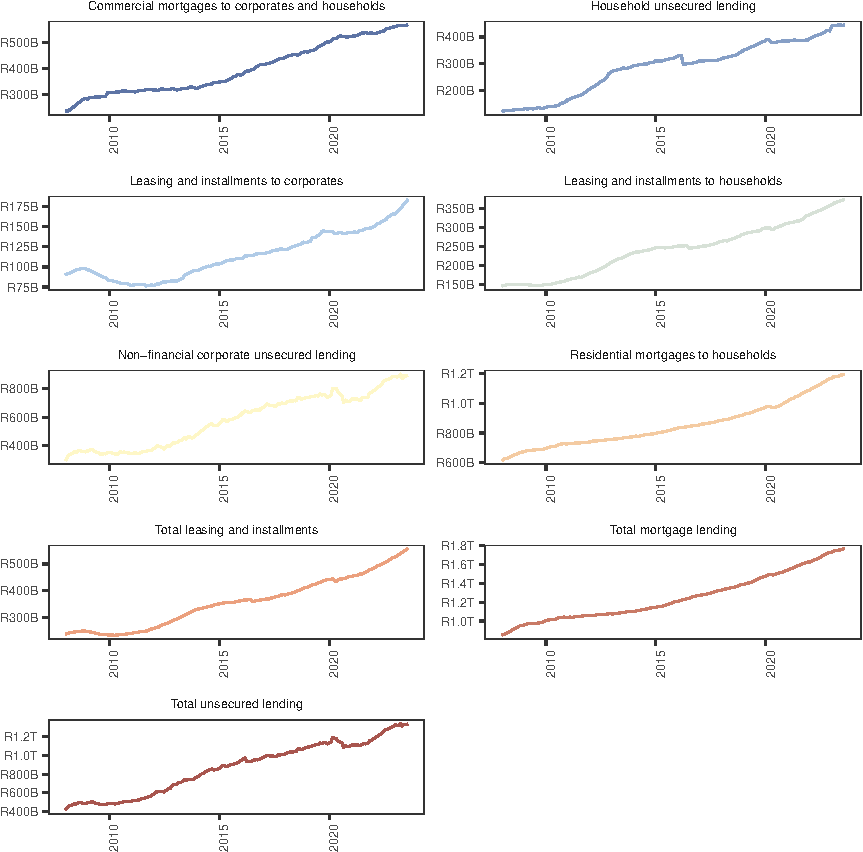
\includegraphics{UP_paper_files/figure-pdf/fig-bank_lending-1.pdf}

}

\caption{\label{fig-bank_lending}Total aggregated bank lending}

\end{figure}

\hypertarget{weighted-lending-rates-aggregated}{%
\subsection{Weighted lending rates
(aggregated)}\label{weighted-lending-rates-aggregated}}

\begin{figure}[H]

{\centering 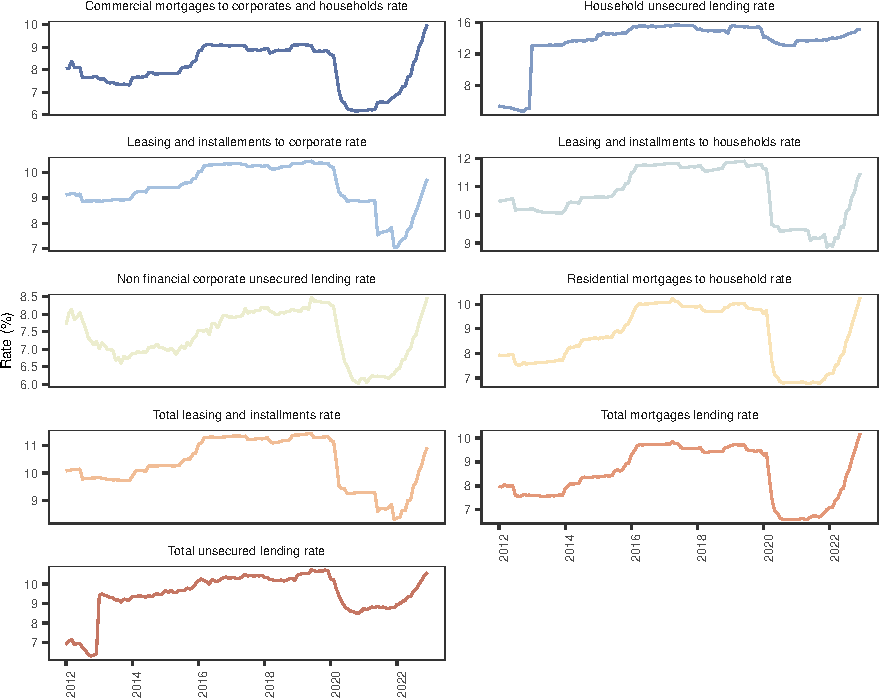
\includegraphics{UP_paper_files/figure-pdf/fig-bank_interest_rates-1.pdf}

}

\caption{\label{fig-bank_interest_rates}Weighted lending rates}

\end{figure}

\newpage

\hypertarget{description-of-narrative-events}{%
\subsection{Description of narrative
events}\label{description-of-narrative-events}}

\hypertarget{macroprudential-indicators}{%
\subsubsection{Macroprudential
Indicators}\label{macroprudential-indicators}}

This section provides a detailed account of the narrative
macroprudential indicators.

2008/01/01: \textcolor{ForestGreen}{Implementation}

\begin{quote}
            BASEL II is  Implemented until Dec 2011

\end{quote}

2009/02/04:
\textcolor{blue}{Announcement, draft and passing of regulation}

\begin{quote}
SARB issues  \textbf{directive 1/2009 (1 of 2009)} announcing the approach banks should follow in the application of capital floors. "Modelled capital should not be below 80\% of the capital requirements under Basel I to ensure capital levels do not fall below prudent level". Following Basel II, banks are allowed to use internal models to determine risk weights and in turn, determine capital levels. However, capital floors ensure capital requirements did not fall below a certain percentage of banks’ capital requirements under the previous Basel I framework\citep{basel06}. This in essence, imply greater risk weight arched to riskier credit products. For instance,  \cite{imbierowicz2018time} show that Danish banks reducing their lending on loans with higher risk weights, in response to higher capital requirements, including approaches to capital floors.
\end{quote}

2009/07/31*:
\textcolor{blue}{Announcement, draft and passing of regulation}

\begin{quote}BCBS announces "measures to strengthen the 1996 rules governing trading book capital and to enhance the three pillars of the Basel II framework (Basel 2.5)". This in essence, aims  to introduce higher capital requirements to capture the credit risk of complex trading activities, promote the build-up of capital buffers that can be drawn down in periods of stress and strengthen the quality of bank capital\citep{basel09}
\end{quote}

2010/10/08*:
\textcolor{blue}{Announcement, draft and passing of regulation}

\begin{quote}SARB issues \textbf{circular 3/2010} endorsing and giving notices to banks to prepare for the implementation of Basel 2.5, following the communication by the BCBS on July 31, 2009
\end{quote}

2011/06/30*:
\textcolor{blue}{Announcement, draft and passing of regulation}

\begin{quote}BCBS issues and publishes Basel III: A Global Regulatory Framework for More Resilient Banks and Banking Systems. ???
\end{quote}

2011/07/31:
\textcolor{blue}{Announcement, draft and passing of regulation}

\begin{quote} 
Cabinet adopts proposal to shift to Twin Peaks Model of Financial Regulation in South Africa, following he GFC, with the aim of improving  institutional structure to support financial regulation. Stricter oversight on finacial system, implications for financial inculsion??
\end{quote}

2011/10/31:
\textcolor{blue}{Announcement, draft and passing of regulation}

\begin{quote}
Basel 2.5 is transposed into domestic law (next step is implementation)
\end{quote}

2012/01/01: \textcolor{ForestGreen}{Implementation}

\begin{quote}
    Basel 2.5 takes effect: SARB minimum capital requirements
    \begin{itemize}
        \item Total CET1, 5.25\%, Total Tier1, 7\%, Minimum regulatory capital, 8\%, Total regulatory capital for D-SIB, 9.5\%
    \end{itemize}
\end{quote}

2012/02/16*:
\textcolor{blue}{Announcement, draft and passing of regulation}

\begin{quote}
SARB issues \textbf{guidance note 2/2012} announcing on new definition of total regulatory capital for Basel III such as:
\begin{itemize}
    \item Phasing out arrangements for non-common equity Tier 1 capital instruments that no longer qualify as regulatory capital under Basel III
 \item Transitional arrangements for Basel III implementation
\item Treatment of disclosed reserves undrer Basel III
\end{itemize}
\end{quote}

2012/05/31*:
\textcolor{blue}{Announcement, draft and passing of regulation}

\begin{quote}
SARB issues \textbf{guidance Note G5/2012} announcing that it will provide  liquidity facility to assist banks in meeting the liquidity Coverage Ratio (LCR) and cash reserves can be included as banks' high quality liquid assets for calculating LCR. This follows results from the QIS exercises by banks,  which revealed some banks would have shortfalls of around R140 billion in meeting the 100\ LCR  by 1 Jan 2019 due do to reliance eon short-term funding limited availability of HQLA

\begin{itemize}
    \item LCR requirements will be introduced on \textbf{1 Jan 2015} at 60\%, increasing by 10\% to reach 100\% on 1 Jan 2019
\item Level 1 assets (stocks, funds or bonds) shall comprise 60\% of total HQLA  while level 2 assets (less liquid) shall constitute no more than the remaining 40\%
\item SARB proposes that Leverage ratio be set at 4\% (LR of 4\% implies that banks' leverage does not exceed its capital by 40\%)
\end{itemize}
\end{quote}

2012/08/15*:
\textcolor{blue}{Announcement, draft and passing of regulation}

\begin{quote}
SARB transposes Basel III into law and publishes Counter-cyclical Capital Buffer (CCyB) rules, set to be implemented on 1 January 2016
\end{quote}

2013/01/31/*: \textcolor{ForestGreen}{Implementation}

\begin{quote}
    Basel III takes effect
\end{quote}

2013/08/20:
\textcolor{blue}{Announcement, draft and passing of regulation}

\begin{quote}
 SARB issues \textbf{Guidance Note 6/2013} announcing that banks' cash reserves may be included as part of their level 1 HQLA. Only equities listed on JSE's main exchange and included on Top 40 Index shall be considered as level2 HQLA (\textit{Potentially limit banks' ability to raise capital}).
\end{quote}

2014/01/31: \textcolor{ForestGreen}{Implementation}

\begin{quote}
SARB mimimum Capital Requirements increase to:\\
Total CET1, 5,5\%, Total Tier1, 7\%, Total regulatory capital, 8\%, Total regulatory capital for D-SIB, 10\%
\end{quote}

2014/12/31:
\textcolor{blue}{Announcement, draft and passing of regulation}

\begin{quote}
SARB issues \textbf{guidance note 8/2014} announcing  the provision of a committed liquidity facility  (CLF). This is to assist banks to meet the LCR.
Banks, however need to have collateral to access the CLF, consisting of:
\begin{itemize}
    \item  High-quality residential mortgage loans
\item Other loans and advances such as VAF, excluding unsecured loans
\item Domestically listed securities
\end{itemize}
\textit{Banks with less diversified asset portfolio, i.e small banks will probably not qualify? Further restrictions/ stricter measures to loan extension?}
\end{quote}

2015/01/31*: \textcolor{ForestGreen}{Implementation}

\begin{quote}
LCR ratio is introduced/impelemnted at 60\% compliance
\end{quote}

2015/12/31*:
\textcolor{blue}{Announcement, draft and passing of regulation}

\begin{quote}

SARB issues \textbf{circular 8/2015} announcing timelines and targets in respect of  the implementation of the countercyclical capital buffer (CCyB). SARB requirements shall apply to bank-wide total RWA:
\begin{itemize}
    \item 0.625\% on 1 Jan 2016
\item 1.25\% 1 Jan 2017
\item 1.875\% on 1 Jan 2018
\item 2.5\% on 1 Jan 2019
\end{itemize}
\end{quote}

2016/01/31*: \textcolor{ForestGreen}{Implementation}

\begin{quote}
LCR ratio is introduced/implemented at 60\% compliance. CCyB also implemented at 0.625\% 
\end{quote}

2016/04/13*:
\textcolor{blue}{Announcement, draft and passing of regulation}

\begin{quote}
SARB issues \textbf{directive 1/2016} to inform all banks of matters related to the exposure limits imposed in the classification of deposits and credit exposures to small and medium enterprises  (SMEs), to be implemented on 1 July 2016. For instance, total exposure of a bank to an SME borrower, which shall be determined or calculated on a consolidated basis, at no time exceeds R12,5 million (\textit{Greater limits on value of a loan that can be extended to an SME and in turn, financial exclusion?})
\end{quote}

2016/07/01*: \textcolor{ForestGreen}{Implementation}

\begin{quote}
Exposure limits imposed in the classification of deposits and credit exposures to small and medium enterprises  (SMEs), announced on 2016/04/13, implemented
\end{quote}

2017/01/31*: \textcolor{ForestGreen}{Implementation}

\begin{quote}
LCR ratio is introduced/implemented at 80\% compliance, while CCyB increases to 1.25\%
\end{quote}

2017/12/13*:
\textcolor{blue}{Announcement, draft and passing of regulation}

\begin{quote}
SARB issues \textbf{directive 8/2017} informing banks to comply with NSFR framework and on matters retaled to calibration of NSFR, including  template to monitor NSFR compliance. Agrees to start implementation on 1 January 2018. Objective is to reduce funding risk over a longer time horizon by requiring banks to fund their activities with sufficiently stable sources of funding in order to mitigate the risk of future funding stress. \textit{anks will be required to match their funding with their outflows, which may lead to a greater demand for longer term funding. Longer term funding will result in an increased cost of funding for banks (possibly passed on to borrowers and lower profitability and returns for banks}
\end{quote}

2018/01/31*: \textcolor{ForestGreen}{Implementation}

\begin{quote}
NSFR Implemented following  Directive 8/2017, CCyB increases to 1,875\% and LCR is implemented at 90\% compliance.
\end{quote}

2019/01/31*: \textcolor{ForestGreen}{Implementation}

\begin{quote}
CCyB increases to 2,5\% (maximum) and LCR is implemented at 100\% compliance.
\end{quote}

\hypertarget{macroprudential-narrative-indexes}{%
\subsection{Macroprudential narrative
indexes}\label{macroprudential-narrative-indexes}}

\begin{figure}[H]

{\centering 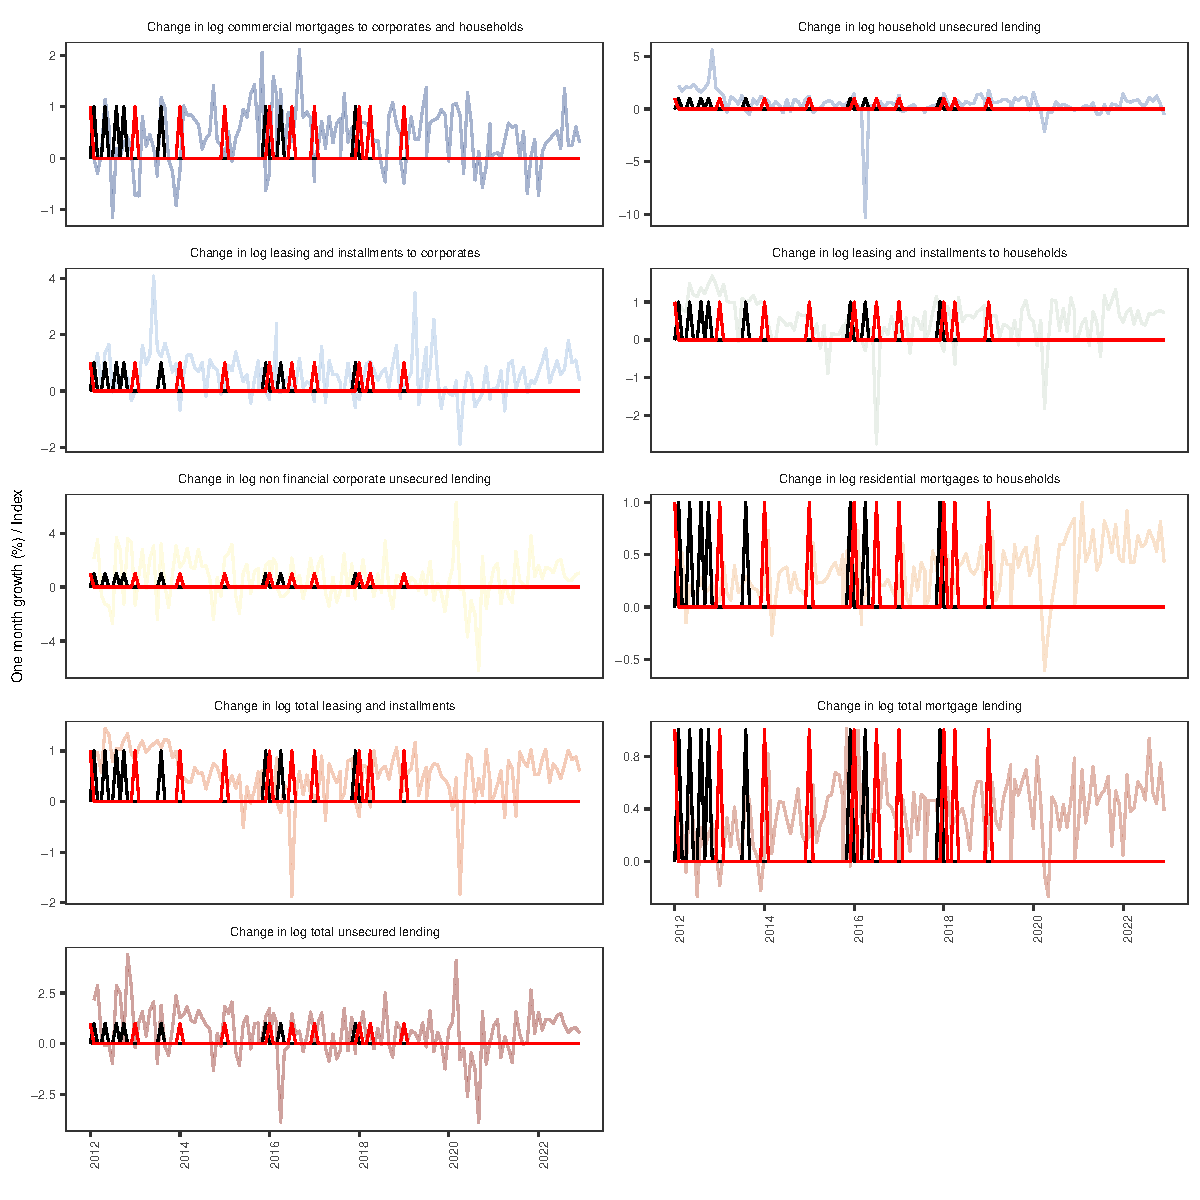
\includegraphics{UP_paper_files/figure-pdf/fig-macro_narrative_indexes_one_month-1.pdf}

}

\caption{\label{fig-macro_narrative_indexes_one_month}One month lending
growth and macroprudential narrative index comparison. Note: The black
line represents the Draft index, and the red line represents the
Implementation index.}

\end{figure}

\newpage

\begin{figure}[H]

{\centering 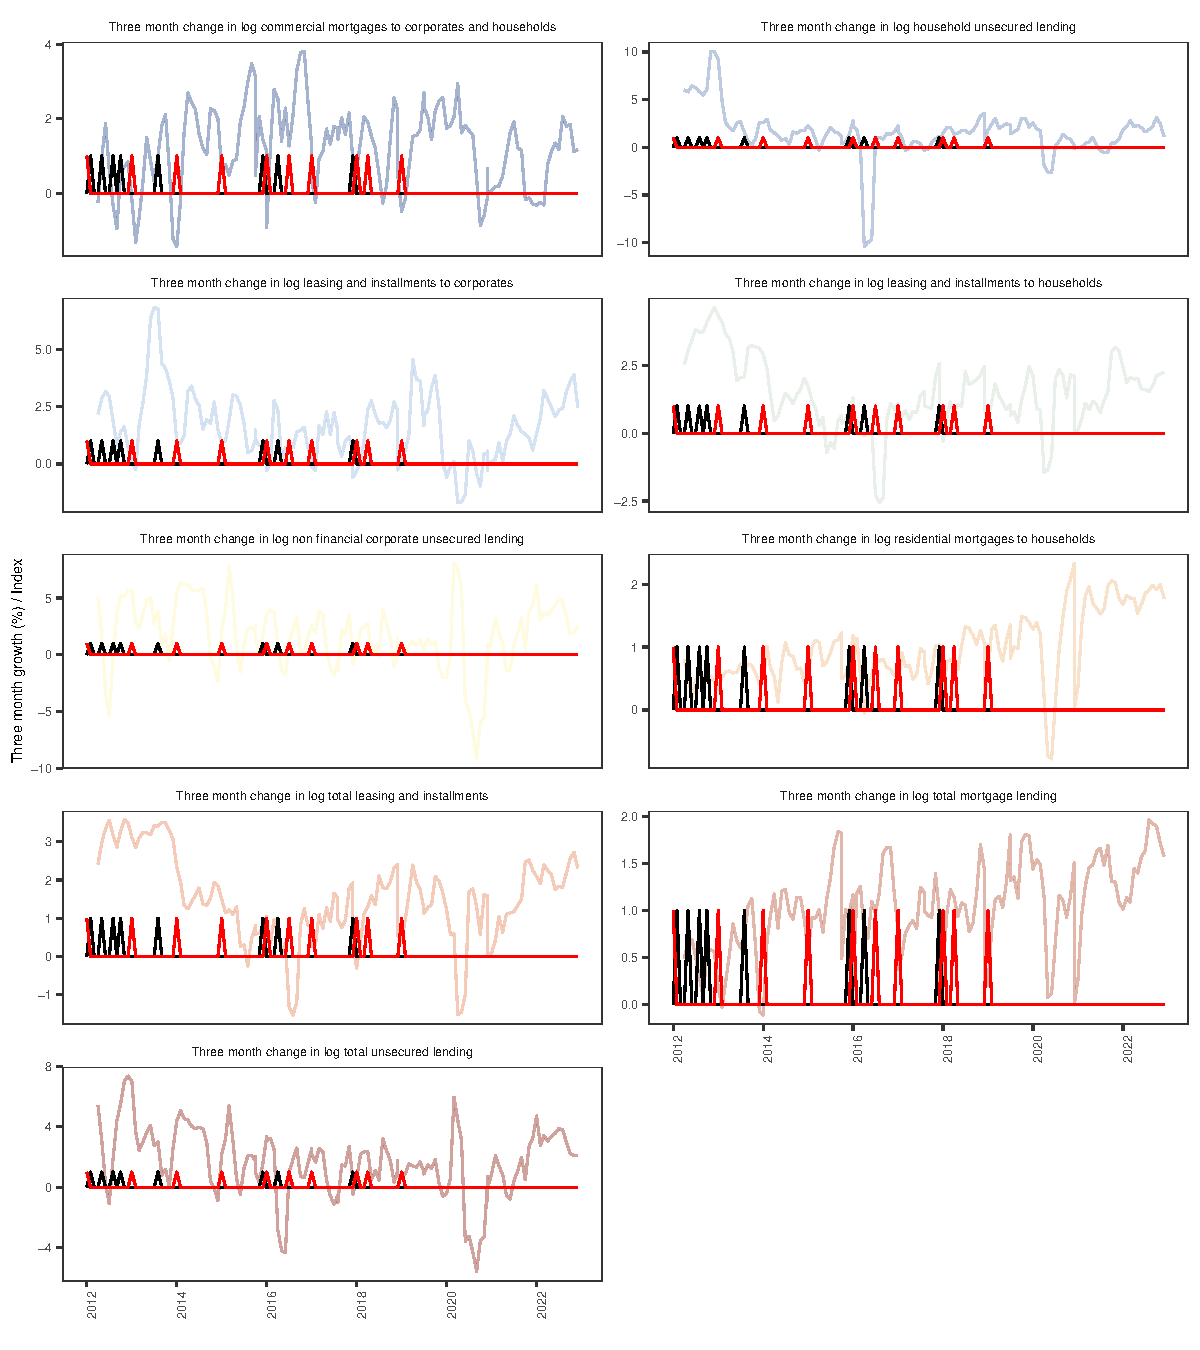
\includegraphics{UP_paper_files/figure-pdf/fig-macro_narrative_indexes_three_month-1.pdf}

}

\caption{\label{fig-macro_narrative_indexes_three_month}Three month
lending growth and macroprudential narrative indexes comparison. Note:
The black line represents the Draft index, and the red line represents
the Implementation index.}

\end{figure}

\newpage

\hypertarget{financial-regulation-narrative-indexes}{%
\subsection{Financial regulation narrative
indexes}\label{financial-regulation-narrative-indexes}}

\begin{figure}[H]

{\centering 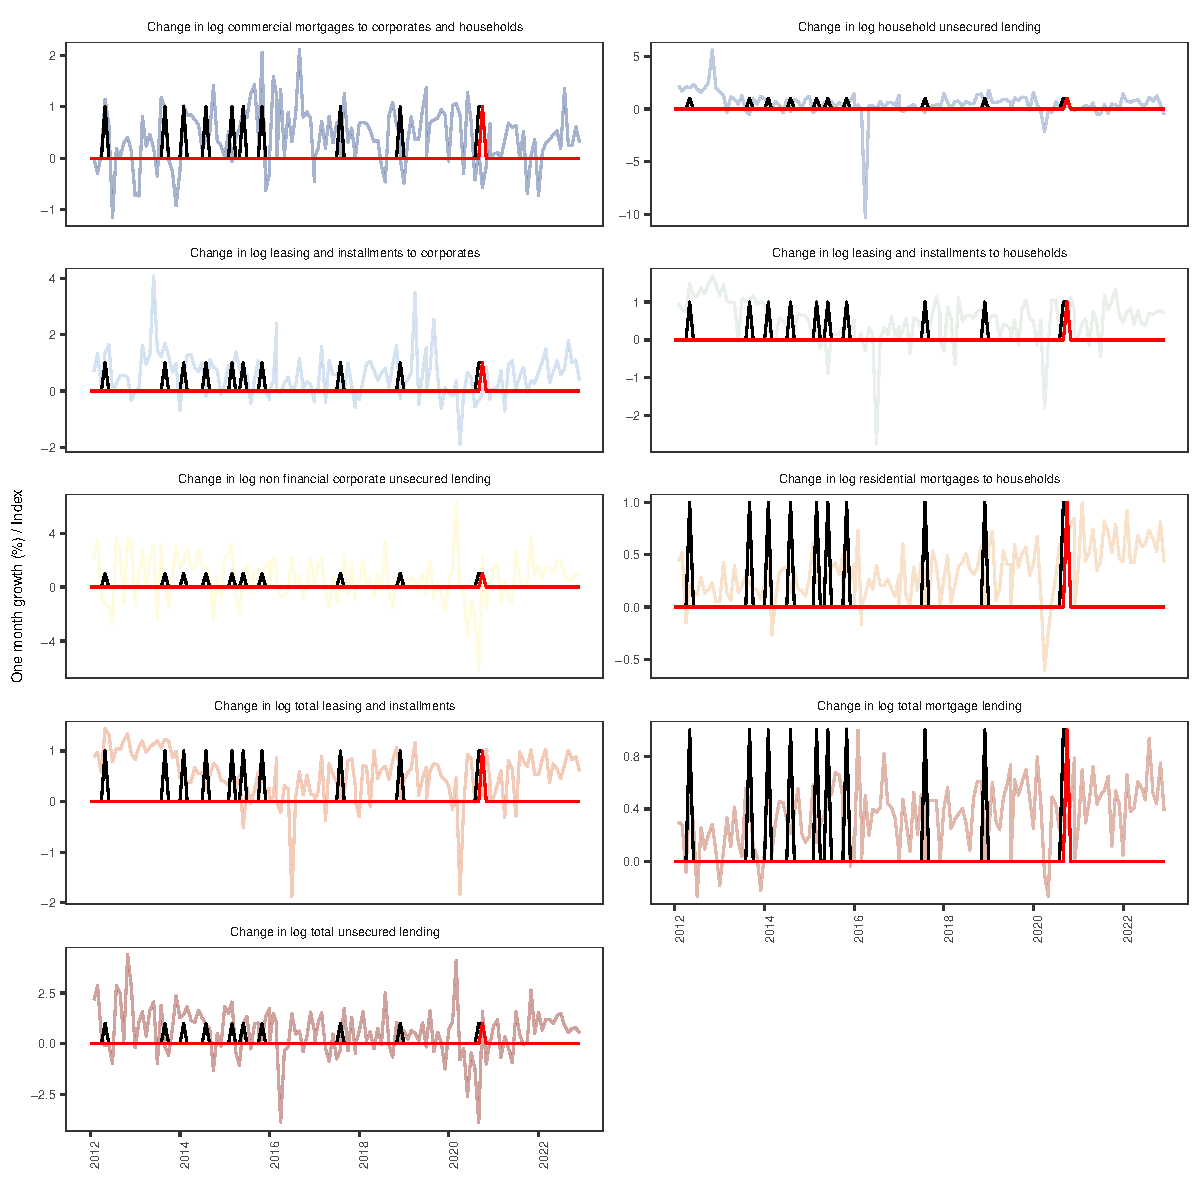
\includegraphics{UP_paper_files/figure-pdf/fig-comp_narrative_indexes_one_month-1.pdf}

}

\caption{\label{fig-comp_narrative_indexes_one_month}One month lending
growth and financial narrative index comparison. Note: The black line
represents the Financial regulation index, and the red line represents
the Financial inclusion index.}

\end{figure}

\newpage

\begin{figure}[H]

{\centering 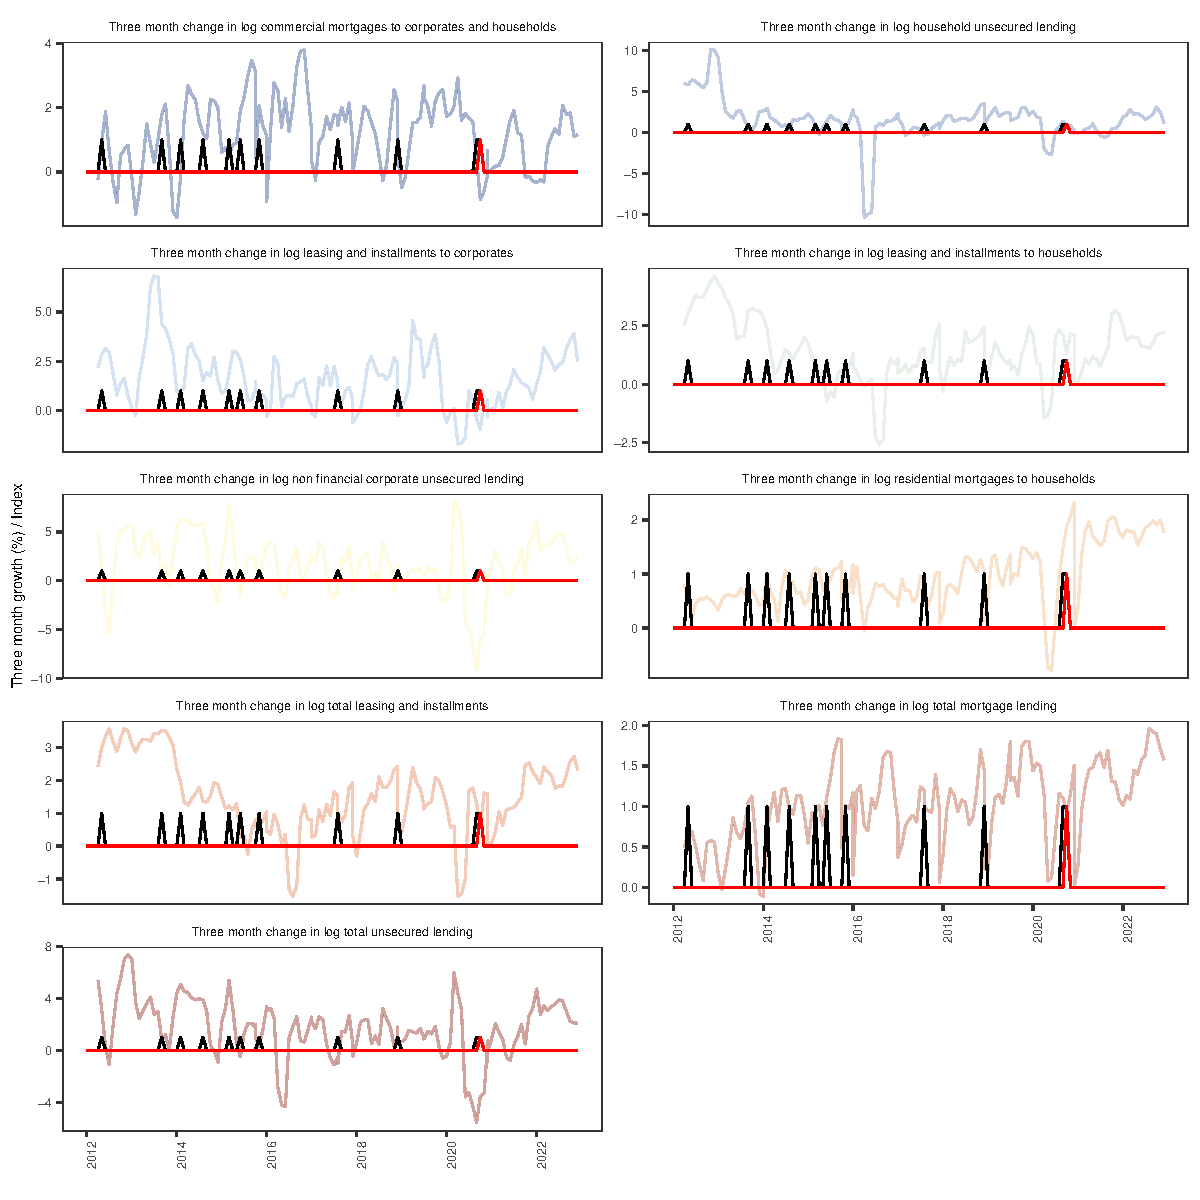
\includegraphics{UP_paper_files/figure-pdf/fig-comp_narrative_indexes_three_month-1.pdf}

}

\caption{\label{fig-comp_narrative_indexes_three_month}Three month
lending growth and financial narrative indexes comparison. Note: The
black line represents the Financial regulation index, and the red line
represents the Financial inclusion index.}

\end{figure}

\newpage

\hypertarget{macropudential-results-with-controls}{%
\subsection{Macropudential results with
controls}\label{macropudential-results-with-controls}}

\bsideways

\hypertarget{tbl-macropru_draft_lending_control}{}
\global\setlength{\Oldarrayrulewidth}{\arrayrulewidth}

\global\setlength{\Oldtabcolsep}{\tabcolsep}

\setlength{\tabcolsep}{2pt}

\renewcommand*{\arraystretch}{1}



\providecommand{\ascline}[3]{\noalign{\global\arrayrulewidth #1}\arrayrulecolor[HTML]{#2}\cline{#3}}

\begin{longtable}[l]{|p{1.40in}|p{0.75in}|p{0.75in}|p{0.75in}|p{0.75in}|p{0.75in}|p{0.75in}|p{0.75in}|p{0.75in}|p{0.75in}}
\caption{\label{tbl-macropru_draft_lending_control}Macroprudential regulations and lending volumes (3-months) with controls
results }\tabularnewline




\ascline{1pt}{000000}{1-10}

\multicolumn{1}{>{\centering}m{\dimexpr 1.4in+0\tabcolsep}}{\textcolor[HTML]{000000}{\fontsize{7}{7}\selectfont{}}} & \multicolumn{3}{!{\color[HTML]{FFFFFF}\vrule width 1pt}>{\centering}m{\dimexpr 2.25in+4\tabcolsep+2pt}}{\textcolor[HTML]{000000}{\fontsize{7}{7}\selectfont{Total}}} & \multicolumn{3}{!{\color[HTML]{FFFFFF}\vrule width 1pt}>{\centering}m{\dimexpr 2.25in+4\tabcolsep+2pt}}{\textcolor[HTML]{000000}{\fontsize{7}{7}\selectfont{Corporates}}} & \multicolumn{3}{!{\color[HTML]{FFFFFF}\vrule width 1pt}>{\centering}m{\dimexpr 2.25in+4\tabcolsep+2pt}!{\color[HTML]{FFFFFF}\vrule width 1pt}}{\textcolor[HTML]{000000}{\fontsize{7}{7}\selectfont{Households}}} \\

\ascline{1pt}{FFFFFF}{1-1}\ascline{1pt}{000000}{2-10}



\multicolumn{1}{>{\raggedright}m{\dimexpr 1.4in+0\tabcolsep}}{\textcolor[HTML]{000000}{\fontsize{7}{7}\selectfont{\ }}} & \multicolumn{1}{!{\color[HTML]{FFFFFF}\vrule width 1pt}>{\raggedright}m{\dimexpr 0.75in+0\tabcolsep}}{\textcolor[HTML]{000000}{\fontsize{7}{7}\selectfont{Unsecured}}} & \multicolumn{1}{!{\color[HTML]{FFFFFF}\vrule width 1pt}>{\raggedright}m{\dimexpr 0.75in+0\tabcolsep}}{\textcolor[HTML]{000000}{\fontsize{7}{7}\selectfont{Secured}}} & \multicolumn{1}{!{\color[HTML]{FFFFFF}\vrule width 1pt}>{\raggedright}m{\dimexpr 0.75in+0\tabcolsep}}{\textcolor[HTML]{000000}{\fontsize{7}{7}\selectfont{Mortgages}}} & \multicolumn{1}{!{\color[HTML]{FFFFFF}\vrule width 1pt}>{\raggedright}m{\dimexpr 0.75in+0\tabcolsep}}{\textcolor[HTML]{000000}{\fontsize{7}{7}\selectfont{Unsecured}}} & \multicolumn{1}{!{\color[HTML]{FFFFFF}\vrule width 1pt}>{\raggedright}m{\dimexpr 0.75in+0\tabcolsep}}{\textcolor[HTML]{000000}{\fontsize{7}{7}\selectfont{Secured}}} & \multicolumn{1}{!{\color[HTML]{FFFFFF}\vrule width 1pt}>{\raggedright}m{\dimexpr 0.75in+0\tabcolsep}}{\textcolor[HTML]{000000}{\fontsize{7}{7}\selectfont{Mortgages}}} & \multicolumn{1}{!{\color[HTML]{FFFFFF}\vrule width 1pt}>{\raggedright}m{\dimexpr 0.75in+0\tabcolsep}}{\textcolor[HTML]{000000}{\fontsize{7}{7}\selectfont{Unsecured}}} & \multicolumn{1}{!{\color[HTML]{FFFFFF}\vrule width 1pt}>{\raggedright}m{\dimexpr 0.75in+0\tabcolsep}}{\textcolor[HTML]{000000}{\fontsize{7}{7}\selectfont{Secured}}} & \multicolumn{1}{!{\color[HTML]{FFFFFF}\vrule width 1pt}>{\raggedright}m{\dimexpr 0.75in+0\tabcolsep}}{\textcolor[HTML]{000000}{\fontsize{7}{7}\selectfont{Mortgages}}} \\

\ascline{1pt}{000000}{1-10}\endfirsthead 

\ascline{1pt}{000000}{1-10}

\multicolumn{1}{>{\centering}m{\dimexpr 1.4in+0\tabcolsep}}{\textcolor[HTML]{000000}{\fontsize{7}{7}\selectfont{}}} & \multicolumn{3}{!{\color[HTML]{FFFFFF}\vrule width 1pt}>{\centering}m{\dimexpr 2.25in+4\tabcolsep+2pt}}{\textcolor[HTML]{000000}{\fontsize{7}{7}\selectfont{Total}}} & \multicolumn{3}{!{\color[HTML]{FFFFFF}\vrule width 1pt}>{\centering}m{\dimexpr 2.25in+4\tabcolsep+2pt}}{\textcolor[HTML]{000000}{\fontsize{7}{7}\selectfont{Corporates}}} & \multicolumn{3}{!{\color[HTML]{FFFFFF}\vrule width 1pt}>{\centering}m{\dimexpr 2.25in+4\tabcolsep+2pt}!{\color[HTML]{FFFFFF}\vrule width 1pt}}{\textcolor[HTML]{000000}{\fontsize{7}{7}\selectfont{Households}}} \\

\ascline{1pt}{FFFFFF}{1-1}\ascline{1pt}{000000}{2-10}



\multicolumn{1}{>{\raggedright}m{\dimexpr 1.4in+0\tabcolsep}}{\textcolor[HTML]{000000}{\fontsize{7}{7}\selectfont{\ }}} & \multicolumn{1}{!{\color[HTML]{FFFFFF}\vrule width 1pt}>{\raggedright}m{\dimexpr 0.75in+0\tabcolsep}}{\textcolor[HTML]{000000}{\fontsize{7}{7}\selectfont{Unsecured}}} & \multicolumn{1}{!{\color[HTML]{FFFFFF}\vrule width 1pt}>{\raggedright}m{\dimexpr 0.75in+0\tabcolsep}}{\textcolor[HTML]{000000}{\fontsize{7}{7}\selectfont{Secured}}} & \multicolumn{1}{!{\color[HTML]{FFFFFF}\vrule width 1pt}>{\raggedright}m{\dimexpr 0.75in+0\tabcolsep}}{\textcolor[HTML]{000000}{\fontsize{7}{7}\selectfont{Mortgages}}} & \multicolumn{1}{!{\color[HTML]{FFFFFF}\vrule width 1pt}>{\raggedright}m{\dimexpr 0.75in+0\tabcolsep}}{\textcolor[HTML]{000000}{\fontsize{7}{7}\selectfont{Unsecured}}} & \multicolumn{1}{!{\color[HTML]{FFFFFF}\vrule width 1pt}>{\raggedright}m{\dimexpr 0.75in+0\tabcolsep}}{\textcolor[HTML]{000000}{\fontsize{7}{7}\selectfont{Secured}}} & \multicolumn{1}{!{\color[HTML]{FFFFFF}\vrule width 1pt}>{\raggedright}m{\dimexpr 0.75in+0\tabcolsep}}{\textcolor[HTML]{000000}{\fontsize{7}{7}\selectfont{Mortgages}}} & \multicolumn{1}{!{\color[HTML]{FFFFFF}\vrule width 1pt}>{\raggedright}m{\dimexpr 0.75in+0\tabcolsep}}{\textcolor[HTML]{000000}{\fontsize{7}{7}\selectfont{Unsecured}}} & \multicolumn{1}{!{\color[HTML]{FFFFFF}\vrule width 1pt}>{\raggedright}m{\dimexpr 0.75in+0\tabcolsep}}{\textcolor[HTML]{000000}{\fontsize{7}{7}\selectfont{Secured}}} & \multicolumn{1}{!{\color[HTML]{FFFFFF}\vrule width 1pt}>{\raggedright}m{\dimexpr 0.75in+0\tabcolsep}}{\textcolor[HTML]{000000}{\fontsize{7}{7}\selectfont{Mortgages}}} \\

\ascline{1pt}{000000}{1-10}\endhead



\multicolumn{10}{>{\centering}m{\dimexpr 8.15in+18\tabcolsep+9pt}!{\color[HTML]{FFFFFF}\vrule width 1pt}}{\textcolor[HTML]{000000}{\fontsize{7}{7}\selectfont{Draft\ model}}} \\

\ascline{1pt}{FFFFFF}{1-10}



\multicolumn{1}{>{\raggedright}m{\dimexpr 1.4in+0\tabcolsep}}{\textcolor[HTML]{000000}{\fontsize{7}{7}\selectfont{Draft\ index}}} & \multicolumn{1}{!{\color[HTML]{FFFFFF}\vrule width 1pt}>{\raggedright}m{\dimexpr 0.75in+0\tabcolsep}}{\textcolor[HTML]{000000}{\fontsize{7}{7}\selectfont{0.64}}} & \multicolumn{1}{!{\color[HTML]{FFFFFF}\vrule width 1pt}>{\raggedright}m{\dimexpr 0.75in+0\tabcolsep}}{\textcolor[HTML]{000000}{\fontsize{7}{7}\selectfont{2.28**}}} & \multicolumn{1}{!{\color[HTML]{FFFFFF}\vrule width 1pt}>{\raggedright}m{\dimexpr 0.75in+0\tabcolsep}}{\textcolor[HTML]{000000}{\fontsize{7}{7}\selectfont{-0.19**}}} & \multicolumn{1}{!{\color[HTML]{FFFFFF}\vrule width 1pt}>{\raggedright}m{\dimexpr 0.75in+0\tabcolsep}}{\textcolor[HTML]{000000}{\fontsize{7}{7}\selectfont{0.42}}} & \multicolumn{1}{!{\color[HTML]{FFFFFF}\vrule width 1pt}>{\raggedright}m{\dimexpr 0.75in+0\tabcolsep}}{\textcolor[HTML]{000000}{\fontsize{7}{7}\selectfont{0.89***}}} & \multicolumn{1}{!{\color[HTML]{FFFFFF}\vrule width 1pt}>{\raggedright}m{\dimexpr 0.75in+0\tabcolsep}}{\textcolor[HTML]{000000}{\fontsize{7}{7}\selectfont{-0.38}}} & \multicolumn{1}{!{\color[HTML]{FFFFFF}\vrule width 1pt}>{\raggedright}m{\dimexpr 0.75in+0\tabcolsep}}{\textcolor[HTML]{000000}{\fontsize{7}{7}\selectfont{1.03**}}} & \multicolumn{1}{!{\color[HTML]{FFFFFF}\vrule width 1pt}>{\raggedright}m{\dimexpr 0.75in+0\tabcolsep}}{\textcolor[HTML]{000000}{\fontsize{7}{7}\selectfont{3.18**}}} & \multicolumn{1}{!{\color[HTML]{FFFFFF}\vrule width 1pt}>{\raggedright}m{\dimexpr 0.75in+0\tabcolsep}}{\textcolor[HTML]{000000}{\fontsize{7}{7}\selectfont{-0.15}}} \\

\ascline{1pt}{FFFFFF}{1-10}



\multicolumn{1}{>{\raggedright}m{\dimexpr 1.4in+0\tabcolsep}}{\textcolor[HTML]{000000}{\fontsize{7}{7}\selectfont{Return\ on\ assets}}} & \multicolumn{1}{!{\color[HTML]{FFFFFF}\vrule width 1pt}>{\raggedright}m{\dimexpr 0.75in+0\tabcolsep}}{\textcolor[HTML]{000000}{\fontsize{7}{7}\selectfont{1.05}}} & \multicolumn{1}{!{\color[HTML]{FFFFFF}\vrule width 1pt}>{\raggedright}m{\dimexpr 0.75in+0\tabcolsep}}{\textcolor[HTML]{000000}{\fontsize{7}{7}\selectfont{-4.14}}} & \multicolumn{1}{!{\color[HTML]{FFFFFF}\vrule width 1pt}>{\raggedright}m{\dimexpr 0.75in+0\tabcolsep}}{\textcolor[HTML]{000000}{\fontsize{7}{7}\selectfont{-0.87}}} & \multicolumn{1}{!{\color[HTML]{FFFFFF}\vrule width 1pt}>{\raggedright}m{\dimexpr 0.75in+0\tabcolsep}}{\textcolor[HTML]{000000}{\fontsize{7}{7}\selectfont{1.50}}} & \multicolumn{1}{!{\color[HTML]{FFFFFF}\vrule width 1pt}>{\raggedright}m{\dimexpr 0.75in+0\tabcolsep}}{\textcolor[HTML]{000000}{\fontsize{7}{7}\selectfont{2.50***}}} & \multicolumn{1}{!{\color[HTML]{FFFFFF}\vrule width 1pt}>{\raggedright}m{\dimexpr 0.75in+0\tabcolsep}}{\textcolor[HTML]{000000}{\fontsize{7}{7}\selectfont{-2.10}}} & \multicolumn{1}{!{\color[HTML]{FFFFFF}\vrule width 1pt}>{\raggedright}m{\dimexpr 0.75in+0\tabcolsep}}{\textcolor[HTML]{000000}{\fontsize{7}{7}\selectfont{-0.61}}} & \multicolumn{1}{!{\color[HTML]{FFFFFF}\vrule width 1pt}>{\raggedright}m{\dimexpr 0.75in+0\tabcolsep}}{\textcolor[HTML]{000000}{\fontsize{7}{7}\selectfont{-7.87}}} & \multicolumn{1}{!{\color[HTML]{FFFFFF}\vrule width 1pt}>{\raggedright}m{\dimexpr 0.75in+0\tabcolsep}}{\textcolor[HTML]{000000}{\fontsize{7}{7}\selectfont{-0.33}}} \\

\ascline{1pt}{FFFFFF}{1-10}



\multicolumn{1}{>{\raggedright}m{\dimexpr 1.4in+0\tabcolsep}}{\textcolor[HTML]{000000}{\fontsize{7}{7}\selectfont{Total\ capital\ adequacy\ ratio}}} & \multicolumn{1}{!{\color[HTML]{FFFFFF}\vrule width 1pt}>{\raggedright}m{\dimexpr 0.75in+0\tabcolsep}}{\textcolor[HTML]{000000}{\fontsize{7}{7}\selectfont{0.23}}} & \multicolumn{1}{!{\color[HTML]{FFFFFF}\vrule width 1pt}>{\raggedright}m{\dimexpr 0.75in+0\tabcolsep}}{\textcolor[HTML]{000000}{\fontsize{7}{7}\selectfont{0.28}}} & \multicolumn{1}{!{\color[HTML]{FFFFFF}\vrule width 1pt}>{\raggedright}m{\dimexpr 0.75in+0\tabcolsep}}{\textcolor[HTML]{000000}{\fontsize{7}{7}\selectfont{0.04}}} & \multicolumn{1}{!{\color[HTML]{FFFFFF}\vrule width 1pt}>{\raggedright}m{\dimexpr 0.75in+0\tabcolsep}}{\textcolor[HTML]{000000}{\fontsize{7}{7}\selectfont{0.19}}} & \multicolumn{1}{!{\color[HTML]{FFFFFF}\vrule width 1pt}>{\raggedright}m{\dimexpr 0.75in+0\tabcolsep}}{\textcolor[HTML]{000000}{\fontsize{7}{7}\selectfont{0.14}}} & \multicolumn{1}{!{\color[HTML]{FFFFFF}\vrule width 1pt}>{\raggedright}m{\dimexpr 0.75in+0\tabcolsep}}{\textcolor[HTML]{000000}{\fontsize{7}{7}\selectfont{0.20}}} & \multicolumn{1}{!{\color[HTML]{FFFFFF}\vrule width 1pt}>{\raggedright}m{\dimexpr 0.75in+0\tabcolsep}}{\textcolor[HTML]{000000}{\fontsize{7}{7}\selectfont{0.35}}} & \multicolumn{1}{!{\color[HTML]{FFFFFF}\vrule width 1pt}>{\raggedright}m{\dimexpr 0.75in+0\tabcolsep}}{\textcolor[HTML]{000000}{\fontsize{7}{7}\selectfont{0.36}}} & \multicolumn{1}{!{\color[HTML]{FFFFFF}\vrule width 1pt}>{\raggedright}m{\dimexpr 0.75in+0\tabcolsep}}{\textcolor[HTML]{000000}{\fontsize{7}{7}\selectfont{0.00}}} \\

\ascline{1pt}{FFFFFF}{1-10}



\multicolumn{10}{>{\centering}m{\dimexpr 8.15in+18\tabcolsep+9pt}!{\color[HTML]{FFFFFF}\vrule width 1pt}}{\textcolor[HTML]{000000}{\fontsize{7}{7}\selectfont{Implementation\ model}}} \\

\ascline{1pt}{FFFFFF}{1-10}



\multicolumn{1}{>{\raggedright}m{\dimexpr 1.4in+0\tabcolsep}}{\textcolor[HTML]{000000}{\fontsize{7}{7}\selectfont{Implementation\ index}}} & \multicolumn{1}{!{\color[HTML]{FFFFFF}\vrule width 1pt}>{\raggedright}m{\dimexpr 0.75in+0\tabcolsep}}{\textcolor[HTML]{000000}{\fontsize{7}{7}\selectfont{1.52***}}} & \multicolumn{1}{!{\color[HTML]{FFFFFF}\vrule width 1pt}>{\raggedright}m{\dimexpr 0.75in+0\tabcolsep}}{\textcolor[HTML]{000000}{\fontsize{7}{7}\selectfont{1.19}}} & \multicolumn{1}{!{\color[HTML]{FFFFFF}\vrule width 1pt}>{\raggedright}m{\dimexpr 0.75in+0\tabcolsep}}{\textcolor[HTML]{000000}{\fontsize{7}{7}\selectfont{-0.49**}}} & \multicolumn{1}{!{\color[HTML]{FFFFFF}\vrule width 1pt}>{\raggedright}m{\dimexpr 0.75in+0\tabcolsep}}{\textcolor[HTML]{000000}{\fontsize{7}{7}\selectfont{1.98***}}} & \multicolumn{1}{!{\color[HTML]{FFFFFF}\vrule width 1pt}>{\raggedright}m{\dimexpr 0.75in+0\tabcolsep}}{\textcolor[HTML]{000000}{\fontsize{7}{7}\selectfont{0.69}}} & \multicolumn{1}{!{\color[HTML]{FFFFFF}\vrule width 1pt}>{\raggedright}m{\dimexpr 0.75in+0\tabcolsep}}{\textcolor[HTML]{000000}{\fontsize{7}{7}\selectfont{-1.18**}}} & \multicolumn{1}{!{\color[HTML]{FFFFFF}\vrule width 1pt}>{\raggedright}m{\dimexpr 0.75in+0\tabcolsep}}{\textcolor[HTML]{000000}{\fontsize{7}{7}\selectfont{0.55}}} & \multicolumn{1}{!{\color[HTML]{FFFFFF}\vrule width 1pt}>{\raggedright}m{\dimexpr 0.75in+0\tabcolsep}}{\textcolor[HTML]{000000}{\fontsize{7}{7}\selectfont{1.29}}} & \multicolumn{1}{!{\color[HTML]{FFFFFF}\vrule width 1pt}>{\raggedright}m{\dimexpr 0.75in+0\tabcolsep}}{\textcolor[HTML]{000000}{\fontsize{7}{7}\selectfont{-0.21*}}} \\

\ascline{1pt}{FFFFFF}{1-10}



\multicolumn{1}{>{\raggedright}m{\dimexpr 1.4in+0\tabcolsep}}{\textcolor[HTML]{000000}{\fontsize{7}{7}\selectfont{Return\ on\ assets}}} & \multicolumn{1}{!{\color[HTML]{FFFFFF}\vrule width 1pt}>{\raggedright}m{\dimexpr 0.75in+0\tabcolsep}}{\textcolor[HTML]{000000}{\fontsize{7}{7}\selectfont{0.87}}} & \multicolumn{1}{!{\color[HTML]{FFFFFF}\vrule width 1pt}>{\raggedright}m{\dimexpr 0.75in+0\tabcolsep}}{\textcolor[HTML]{000000}{\fontsize{7}{7}\selectfont{-4.26}}} & \multicolumn{1}{!{\color[HTML]{FFFFFF}\vrule width 1pt}>{\raggedright}m{\dimexpr 0.75in+0\tabcolsep}}{\textcolor[HTML]{000000}{\fontsize{7}{7}\selectfont{-0.81}}} & \multicolumn{1}{!{\color[HTML]{FFFFFF}\vrule width 1pt}>{\raggedright}m{\dimexpr 0.75in+0\tabcolsep}}{\textcolor[HTML]{000000}{\fontsize{7}{7}\selectfont{1.26}}} & \multicolumn{1}{!{\color[HTML]{FFFFFF}\vrule width 1pt}>{\raggedright}m{\dimexpr 0.75in+0\tabcolsep}}{\textcolor[HTML]{000000}{\fontsize{7}{7}\selectfont{2.43*}}} & \multicolumn{1}{!{\color[HTML]{FFFFFF}\vrule width 1pt}>{\raggedright}m{\dimexpr 0.75in+0\tabcolsep}}{\textcolor[HTML]{000000}{\fontsize{7}{7}\selectfont{-1.96}}} & \multicolumn{1}{!{\color[HTML]{FFFFFF}\vrule width 1pt}>{\raggedright}m{\dimexpr 0.75in+0\tabcolsep}}{\textcolor[HTML]{000000}{\fontsize{7}{7}\selectfont{-0.67}}} & \multicolumn{1}{!{\color[HTML]{FFFFFF}\vrule width 1pt}>{\raggedright}m{\dimexpr 0.75in+0\tabcolsep}}{\textcolor[HTML]{000000}{\fontsize{7}{7}\selectfont{-7.98}}} & \multicolumn{1}{!{\color[HTML]{FFFFFF}\vrule width 1pt}>{\raggedright}m{\dimexpr 0.75in+0\tabcolsep}}{\textcolor[HTML]{000000}{\fontsize{7}{7}\selectfont{-0.31}}} \\

\ascline{1pt}{FFFFFF}{1-10}



\multicolumn{1}{>{\raggedright}m{\dimexpr 1.4in+0\tabcolsep}}{\textcolor[HTML]{000000}{\fontsize{7}{7}\selectfont{Total\ capital\ adequacy\ ratio}}} & \multicolumn{1}{!{\color[HTML]{FFFFFF}\vrule width 1pt}>{\raggedright}m{\dimexpr 0.75in+0\tabcolsep}}{\textcolor[HTML]{000000}{\fontsize{7}{7}\selectfont{0.21}}} & \multicolumn{1}{!{\color[HTML]{FFFFFF}\vrule width 1pt}>{\raggedright}m{\dimexpr 0.75in+0\tabcolsep}}{\textcolor[HTML]{000000}{\fontsize{7}{7}\selectfont{0.25}}} & \multicolumn{1}{!{\color[HTML]{FFFFFF}\vrule width 1pt}>{\raggedright}m{\dimexpr 0.75in+0\tabcolsep}}{\textcolor[HTML]{000000}{\fontsize{7}{7}\selectfont{0.04}}} & \multicolumn{1}{!{\color[HTML]{FFFFFF}\vrule width 1pt}>{\raggedright}m{\dimexpr 0.75in+0\tabcolsep}}{\textcolor[HTML]{000000}{\fontsize{7}{7}\selectfont{0.16}}} & \multicolumn{1}{!{\color[HTML]{FFFFFF}\vrule width 1pt}>{\raggedright}m{\dimexpr 0.75in+0\tabcolsep}}{\textcolor[HTML]{000000}{\fontsize{7}{7}\selectfont{0.13}}} & \multicolumn{1}{!{\color[HTML]{FFFFFF}\vrule width 1pt}>{\raggedright}m{\dimexpr 0.75in+0\tabcolsep}}{\textcolor[HTML]{000000}{\fontsize{7}{7}\selectfont{0.22}}} & \multicolumn{1}{!{\color[HTML]{FFFFFF}\vrule width 1pt}>{\raggedright}m{\dimexpr 0.75in+0\tabcolsep}}{\textcolor[HTML]{000000}{\fontsize{7}{7}\selectfont{0.34}}} & \multicolumn{1}{!{\color[HTML]{FFFFFF}\vrule width 1pt}>{\raggedright}m{\dimexpr 0.75in+0\tabcolsep}}{\textcolor[HTML]{000000}{\fontsize{7}{7}\selectfont{0.33}}} & \multicolumn{1}{!{\color[HTML]{FFFFFF}\vrule width 1pt}>{\raggedright}m{\dimexpr 0.75in+0\tabcolsep}}{\textcolor[HTML]{000000}{\fontsize{7}{7}\selectfont{0.00}}} \\

\ascline{1pt}{000000}{1-10}



\multicolumn{1}{>{\raggedright}m{\dimexpr 1.4in+0\tabcolsep}}{\textcolor[HTML]{000000}{\fontsize{7}{7}\selectfont{Num.Obs.}}} & \multicolumn{1}{!{\color[HTML]{FFFFFF}\vrule width 1pt}>{\raggedright}m{\dimexpr 0.75in+0\tabcolsep}}{\textcolor[HTML]{000000}{\fontsize{7}{7}\selectfont{580}}} & \multicolumn{1}{!{\color[HTML]{FFFFFF}\vrule width 1pt}>{\raggedright}m{\dimexpr 0.75in+0\tabcolsep}}{\textcolor[HTML]{000000}{\fontsize{7}{7}\selectfont{580}}} & \multicolumn{1}{!{\color[HTML]{FFFFFF}\vrule width 1pt}>{\raggedright}m{\dimexpr 0.75in+0\tabcolsep}}{\textcolor[HTML]{000000}{\fontsize{7}{7}\selectfont{580}}} & \multicolumn{1}{!{\color[HTML]{FFFFFF}\vrule width 1pt}>{\raggedright}m{\dimexpr 0.75in+0\tabcolsep}}{\textcolor[HTML]{000000}{\fontsize{7}{7}\selectfont{580}}} & \multicolumn{1}{!{\color[HTML]{FFFFFF}\vrule width 1pt}>{\raggedright}m{\dimexpr 0.75in+0\tabcolsep}}{\textcolor[HTML]{000000}{\fontsize{7}{7}\selectfont{580}}} & \multicolumn{1}{!{\color[HTML]{FFFFFF}\vrule width 1pt}>{\raggedright}m{\dimexpr 0.75in+0\tabcolsep}}{\textcolor[HTML]{000000}{\fontsize{7}{7}\selectfont{580}}} & \multicolumn{1}{!{\color[HTML]{FFFFFF}\vrule width 1pt}>{\raggedright}m{\dimexpr 0.75in+0\tabcolsep}}{\textcolor[HTML]{000000}{\fontsize{7}{7}\selectfont{580}}} & \multicolumn{1}{!{\color[HTML]{FFFFFF}\vrule width 1pt}>{\raggedright}m{\dimexpr 0.75in+0\tabcolsep}}{\textcolor[HTML]{000000}{\fontsize{7}{7}\selectfont{580}}} & \multicolumn{1}{!{\color[HTML]{FFFFFF}\vrule width 1pt}>{\raggedright}m{\dimexpr 0.75in+0\tabcolsep}}{\textcolor[HTML]{000000}{\fontsize{7}{7}\selectfont{580}}} \\

\ascline{1pt}{FFFFFF}{1-10}



\multicolumn{1}{>{\raggedright}m{\dimexpr 1.4in+0\tabcolsep}}{\textcolor[HTML]{000000}{\fontsize{7}{7}\selectfont{Bank\ Fixed\ Effects}}} & \multicolumn{1}{!{\color[HTML]{FFFFFF}\vrule width 1pt}>{\raggedright}m{\dimexpr 0.75in+0\tabcolsep}}{\textcolor[HTML]{000000}{\fontsize{7}{7}\selectfont{Yes}}} & \multicolumn{1}{!{\color[HTML]{FFFFFF}\vrule width 1pt}>{\raggedright}m{\dimexpr 0.75in+0\tabcolsep}}{\textcolor[HTML]{000000}{\fontsize{7}{7}\selectfont{Yes}}} & \multicolumn{1}{!{\color[HTML]{FFFFFF}\vrule width 1pt}>{\raggedright}m{\dimexpr 0.75in+0\tabcolsep}}{\textcolor[HTML]{000000}{\fontsize{7}{7}\selectfont{Yes}}} & \multicolumn{1}{!{\color[HTML]{FFFFFF}\vrule width 1pt}>{\raggedright}m{\dimexpr 0.75in+0\tabcolsep}}{\textcolor[HTML]{000000}{\fontsize{7}{7}\selectfont{Yes}}} & \multicolumn{1}{!{\color[HTML]{FFFFFF}\vrule width 1pt}>{\raggedright}m{\dimexpr 0.75in+0\tabcolsep}}{\textcolor[HTML]{000000}{\fontsize{7}{7}\selectfont{Yes}}} & \multicolumn{1}{!{\color[HTML]{FFFFFF}\vrule width 1pt}>{\raggedright}m{\dimexpr 0.75in+0\tabcolsep}}{\textcolor[HTML]{000000}{\fontsize{7}{7}\selectfont{Yes}}} & \multicolumn{1}{!{\color[HTML]{FFFFFF}\vrule width 1pt}>{\raggedright}m{\dimexpr 0.75in+0\tabcolsep}}{\textcolor[HTML]{000000}{\fontsize{7}{7}\selectfont{Yes}}} & \multicolumn{1}{!{\color[HTML]{FFFFFF}\vrule width 1pt}>{\raggedright}m{\dimexpr 0.75in+0\tabcolsep}}{\textcolor[HTML]{000000}{\fontsize{7}{7}\selectfont{Yes}}} & \multicolumn{1}{!{\color[HTML]{FFFFFF}\vrule width 1pt}>{\raggedright}m{\dimexpr 0.75in+0\tabcolsep}}{\textcolor[HTML]{000000}{\fontsize{7}{7}\selectfont{Yes}}} \\

\ascline{1pt}{FFFFFF}{1-10}



\multicolumn{1}{>{\raggedright}m{\dimexpr 1.4in+0\tabcolsep}}{\textcolor[HTML]{000000}{\fontsize{7}{7}\selectfont{Monthly\ Fixed\ Effects}}} & \multicolumn{1}{!{\color[HTML]{FFFFFF}\vrule width 1pt}>{\raggedright}m{\dimexpr 0.75in+0\tabcolsep}}{\textcolor[HTML]{000000}{\fontsize{7}{7}\selectfont{Yes}}} & \multicolumn{1}{!{\color[HTML]{FFFFFF}\vrule width 1pt}>{\raggedright}m{\dimexpr 0.75in+0\tabcolsep}}{\textcolor[HTML]{000000}{\fontsize{7}{7}\selectfont{Yes}}} & \multicolumn{1}{!{\color[HTML]{FFFFFF}\vrule width 1pt}>{\raggedright}m{\dimexpr 0.75in+0\tabcolsep}}{\textcolor[HTML]{000000}{\fontsize{7}{7}\selectfont{Yes}}} & \multicolumn{1}{!{\color[HTML]{FFFFFF}\vrule width 1pt}>{\raggedright}m{\dimexpr 0.75in+0\tabcolsep}}{\textcolor[HTML]{000000}{\fontsize{7}{7}\selectfont{Yes}}} & \multicolumn{1}{!{\color[HTML]{FFFFFF}\vrule width 1pt}>{\raggedright}m{\dimexpr 0.75in+0\tabcolsep}}{\textcolor[HTML]{000000}{\fontsize{7}{7}\selectfont{Yes}}} & \multicolumn{1}{!{\color[HTML]{FFFFFF}\vrule width 1pt}>{\raggedright}m{\dimexpr 0.75in+0\tabcolsep}}{\textcolor[HTML]{000000}{\fontsize{7}{7}\selectfont{Yes}}} & \multicolumn{1}{!{\color[HTML]{FFFFFF}\vrule width 1pt}>{\raggedright}m{\dimexpr 0.75in+0\tabcolsep}}{\textcolor[HTML]{000000}{\fontsize{7}{7}\selectfont{Yes}}} & \multicolumn{1}{!{\color[HTML]{FFFFFF}\vrule width 1pt}>{\raggedright}m{\dimexpr 0.75in+0\tabcolsep}}{\textcolor[HTML]{000000}{\fontsize{7}{7}\selectfont{Yes}}} & \multicolumn{1}{!{\color[HTML]{FFFFFF}\vrule width 1pt}>{\raggedright}m{\dimexpr 0.75in+0\tabcolsep}}{\textcolor[HTML]{000000}{\fontsize{7}{7}\selectfont{Yes}}} \\

\ascline{1pt}{000000}{1-10}



\multicolumn{10}{>{\raggedright}m{\dimexpr 8.15in+18\tabcolsep+9pt}!{\color[HTML]{FFFFFF}\vrule width 1pt}}{\textcolor[HTML]{000000}{\fontsize{7}{7}\selectfont{*\ p\ <\ 0.1,\ **\ p\ <\ 0.05,\ ***\ p\ <\ 0.01}}} \\

\ascline{1pt}{000000}{1-10}



\end{longtable}



\arrayrulecolor[HTML]{000000}

\global\setlength{\arrayrulewidth}{\Oldarrayrulewidth}

\global\setlength{\tabcolsep}{\Oldtabcolsep}

\renewcommand*{\arraystretch}{1}

\esideways

\bsideways

\hypertarget{tbl-macropru_draft_rates_control}{}
\global\setlength{\Oldarrayrulewidth}{\arrayrulewidth}

\global\setlength{\Oldtabcolsep}{\tabcolsep}

\setlength{\tabcolsep}{2pt}

\renewcommand*{\arraystretch}{1}



\providecommand{\ascline}[3]{\noalign{\global\arrayrulewidth #1}\arrayrulecolor[HTML]{#2}\cline{#3}}

\begin{longtable}[l]{|p{1.40in}|p{0.75in}|p{0.75in}|p{0.75in}|p{0.75in}|p{0.75in}|p{0.75in}|p{0.75in}|p{0.75in}|p{0.75in}}
\caption{\label{tbl-macropru_draft_rates_control}Macroprudential regulation and lending rates with controls results }\tabularnewline




\ascline{1pt}{000000}{1-10}

\multicolumn{1}{>{\centering}m{\dimexpr 1.4in+0\tabcolsep}}{\textcolor[HTML]{000000}{\fontsize{7}{7}\selectfont{}}} & \multicolumn{3}{!{\color[HTML]{FFFFFF}\vrule width 1pt}>{\centering}m{\dimexpr 2.25in+4\tabcolsep+2pt}}{\textcolor[HTML]{000000}{\fontsize{7}{7}\selectfont{Total}}} & \multicolumn{3}{!{\color[HTML]{FFFFFF}\vrule width 1pt}>{\centering}m{\dimexpr 2.25in+4\tabcolsep+2pt}}{\textcolor[HTML]{000000}{\fontsize{7}{7}\selectfont{Corporations}}} & \multicolumn{3}{!{\color[HTML]{FFFFFF}\vrule width 1pt}>{\centering}m{\dimexpr 2.25in+4\tabcolsep+2pt}!{\color[HTML]{FFFFFF}\vrule width 1pt}}{\textcolor[HTML]{000000}{\fontsize{7}{7}\selectfont{Households}}} \\

\ascline{1pt}{FFFFFF}{1-1}\ascline{1pt}{000000}{2-10}



\multicolumn{1}{>{\raggedright}m{\dimexpr 1.4in+0\tabcolsep}}{\textcolor[HTML]{000000}{\fontsize{7}{7}\selectfont{\ }}} & \multicolumn{1}{!{\color[HTML]{FFFFFF}\vrule width 1pt}>{\raggedright}m{\dimexpr 0.75in+0\tabcolsep}}{\textcolor[HTML]{000000}{\fontsize{7}{7}\selectfont{Unsecured}}} & \multicolumn{1}{!{\color[HTML]{FFFFFF}\vrule width 1pt}>{\raggedright}m{\dimexpr 0.75in+0\tabcolsep}}{\textcolor[HTML]{000000}{\fontsize{7}{7}\selectfont{Secured}}} & \multicolumn{1}{!{\color[HTML]{FFFFFF}\vrule width 1pt}>{\raggedright}m{\dimexpr 0.75in+0\tabcolsep}}{\textcolor[HTML]{000000}{\fontsize{7}{7}\selectfont{Mortgage}}} & \multicolumn{1}{!{\color[HTML]{FFFFFF}\vrule width 1pt}>{\raggedright}m{\dimexpr 0.75in+0\tabcolsep}}{\textcolor[HTML]{000000}{\fontsize{7}{7}\selectfont{Unsecured}}} & \multicolumn{1}{!{\color[HTML]{FFFFFF}\vrule width 1pt}>{\raggedright}m{\dimexpr 0.75in+0\tabcolsep}}{\textcolor[HTML]{000000}{\fontsize{7}{7}\selectfont{Secured}}} & \multicolumn{1}{!{\color[HTML]{FFFFFF}\vrule width 1pt}>{\raggedright}m{\dimexpr 0.75in+0\tabcolsep}}{\textcolor[HTML]{000000}{\fontsize{7}{7}\selectfont{Mortgage}}} & \multicolumn{1}{!{\color[HTML]{FFFFFF}\vrule width 1pt}>{\raggedright}m{\dimexpr 0.75in+0\tabcolsep}}{\textcolor[HTML]{000000}{\fontsize{7}{7}\selectfont{Unsecured}}} & \multicolumn{1}{!{\color[HTML]{FFFFFF}\vrule width 1pt}>{\raggedright}m{\dimexpr 0.75in+0\tabcolsep}}{\textcolor[HTML]{000000}{\fontsize{7}{7}\selectfont{Secured}}} & \multicolumn{1}{!{\color[HTML]{FFFFFF}\vrule width 1pt}>{\raggedright}m{\dimexpr 0.75in+0\tabcolsep}}{\textcolor[HTML]{000000}{\fontsize{7}{7}\selectfont{Mortgage}}} \\

\ascline{1pt}{000000}{1-10}\endfirsthead 

\ascline{1pt}{000000}{1-10}

\multicolumn{1}{>{\centering}m{\dimexpr 1.4in+0\tabcolsep}}{\textcolor[HTML]{000000}{\fontsize{7}{7}\selectfont{}}} & \multicolumn{3}{!{\color[HTML]{FFFFFF}\vrule width 1pt}>{\centering}m{\dimexpr 2.25in+4\tabcolsep+2pt}}{\textcolor[HTML]{000000}{\fontsize{7}{7}\selectfont{Total}}} & \multicolumn{3}{!{\color[HTML]{FFFFFF}\vrule width 1pt}>{\centering}m{\dimexpr 2.25in+4\tabcolsep+2pt}}{\textcolor[HTML]{000000}{\fontsize{7}{7}\selectfont{Corporations}}} & \multicolumn{3}{!{\color[HTML]{FFFFFF}\vrule width 1pt}>{\centering}m{\dimexpr 2.25in+4\tabcolsep+2pt}!{\color[HTML]{FFFFFF}\vrule width 1pt}}{\textcolor[HTML]{000000}{\fontsize{7}{7}\selectfont{Households}}} \\

\ascline{1pt}{FFFFFF}{1-1}\ascline{1pt}{000000}{2-10}



\multicolumn{1}{>{\raggedright}m{\dimexpr 1.4in+0\tabcolsep}}{\textcolor[HTML]{000000}{\fontsize{7}{7}\selectfont{\ }}} & \multicolumn{1}{!{\color[HTML]{FFFFFF}\vrule width 1pt}>{\raggedright}m{\dimexpr 0.75in+0\tabcolsep}}{\textcolor[HTML]{000000}{\fontsize{7}{7}\selectfont{Unsecured}}} & \multicolumn{1}{!{\color[HTML]{FFFFFF}\vrule width 1pt}>{\raggedright}m{\dimexpr 0.75in+0\tabcolsep}}{\textcolor[HTML]{000000}{\fontsize{7}{7}\selectfont{Secured}}} & \multicolumn{1}{!{\color[HTML]{FFFFFF}\vrule width 1pt}>{\raggedright}m{\dimexpr 0.75in+0\tabcolsep}}{\textcolor[HTML]{000000}{\fontsize{7}{7}\selectfont{Mortgage}}} & \multicolumn{1}{!{\color[HTML]{FFFFFF}\vrule width 1pt}>{\raggedright}m{\dimexpr 0.75in+0\tabcolsep}}{\textcolor[HTML]{000000}{\fontsize{7}{7}\selectfont{Unsecured}}} & \multicolumn{1}{!{\color[HTML]{FFFFFF}\vrule width 1pt}>{\raggedright}m{\dimexpr 0.75in+0\tabcolsep}}{\textcolor[HTML]{000000}{\fontsize{7}{7}\selectfont{Secured}}} & \multicolumn{1}{!{\color[HTML]{FFFFFF}\vrule width 1pt}>{\raggedright}m{\dimexpr 0.75in+0\tabcolsep}}{\textcolor[HTML]{000000}{\fontsize{7}{7}\selectfont{Mortgage}}} & \multicolumn{1}{!{\color[HTML]{FFFFFF}\vrule width 1pt}>{\raggedright}m{\dimexpr 0.75in+0\tabcolsep}}{\textcolor[HTML]{000000}{\fontsize{7}{7}\selectfont{Unsecured}}} & \multicolumn{1}{!{\color[HTML]{FFFFFF}\vrule width 1pt}>{\raggedright}m{\dimexpr 0.75in+0\tabcolsep}}{\textcolor[HTML]{000000}{\fontsize{7}{7}\selectfont{Secured}}} & \multicolumn{1}{!{\color[HTML]{FFFFFF}\vrule width 1pt}>{\raggedright}m{\dimexpr 0.75in+0\tabcolsep}}{\textcolor[HTML]{000000}{\fontsize{7}{7}\selectfont{Mortgage}}} \\

\ascline{1pt}{000000}{1-10}\endhead



\multicolumn{10}{>{\centering}m{\dimexpr 8.15in+18\tabcolsep+9pt}!{\color[HTML]{FFFFFF}\vrule width 1pt}}{\textcolor[HTML]{000000}{\fontsize{7}{7}\selectfont{Draft\ model}}} \\

\ascline{1pt}{FFFFFF}{1-10}



\multicolumn{1}{>{\raggedright}m{\dimexpr 1.4in+0\tabcolsep}}{\textcolor[HTML]{000000}{\fontsize{7}{7}\selectfont{Draft\ index}}} & \multicolumn{1}{!{\color[HTML]{FFFFFF}\vrule width 1pt}>{\raggedright}m{\dimexpr 0.75in+0\tabcolsep}}{\textcolor[HTML]{000000}{\fontsize{7}{7}\selectfont{0.41*}}} & \multicolumn{1}{!{\color[HTML]{FFFFFF}\vrule width 1pt}>{\raggedright}m{\dimexpr 0.75in+0\tabcolsep}}{\textcolor[HTML]{000000}{\fontsize{7}{7}\selectfont{-0.38***}}} & \multicolumn{1}{!{\color[HTML]{FFFFFF}\vrule width 1pt}>{\raggedright}m{\dimexpr 0.75in+0\tabcolsep}}{\textcolor[HTML]{000000}{\fontsize{7}{7}\selectfont{-0.47***}}} & \multicolumn{1}{!{\color[HTML]{FFFFFF}\vrule width 1pt}>{\raggedright}m{\dimexpr 0.75in+0\tabcolsep}}{\textcolor[HTML]{000000}{\fontsize{7}{7}\selectfont{0.36}}} & \multicolumn{1}{!{\color[HTML]{FFFFFF}\vrule width 1pt}>{\raggedright}m{\dimexpr 0.75in+0\tabcolsep}}{\textcolor[HTML]{000000}{\fontsize{7}{7}\selectfont{-0.44***}}} & \multicolumn{1}{!{\color[HTML]{FFFFFF}\vrule width 1pt}>{\raggedright}m{\dimexpr 0.75in+0\tabcolsep}}{\textcolor[HTML]{000000}{\fontsize{7}{7}\selectfont{-0.18}}} & \multicolumn{1}{!{\color[HTML]{FFFFFF}\vrule width 1pt}>{\raggedright}m{\dimexpr 0.75in+0\tabcolsep}}{\textcolor[HTML]{000000}{\fontsize{7}{7}\selectfont{0.39*}}} & \multicolumn{1}{!{\color[HTML]{FFFFFF}\vrule width 1pt}>{\raggedright}m{\dimexpr 0.75in+0\tabcolsep}}{\textcolor[HTML]{000000}{\fontsize{7}{7}\selectfont{-0.35***}}} & \multicolumn{1}{!{\color[HTML]{FFFFFF}\vrule width 1pt}>{\raggedright}m{\dimexpr 0.75in+0\tabcolsep}}{\textcolor[HTML]{000000}{\fontsize{7}{7}\selectfont{-0.57***}}} \\

\ascline{1pt}{FFFFFF}{1-10}



\multicolumn{1}{>{\raggedright}m{\dimexpr 1.4in+0\tabcolsep}}{\textcolor[HTML]{000000}{\fontsize{7}{7}\selectfont{Return\ on\ assets}}} & \multicolumn{1}{!{\color[HTML]{FFFFFF}\vrule width 1pt}>{\raggedright}m{\dimexpr 0.75in+0\tabcolsep}}{\textcolor[HTML]{000000}{\fontsize{7}{7}\selectfont{5.85***}}} & \multicolumn{1}{!{\color[HTML]{FFFFFF}\vrule width 1pt}>{\raggedright}m{\dimexpr 0.75in+0\tabcolsep}}{\textcolor[HTML]{000000}{\fontsize{7}{7}\selectfont{-0.79**}}} & \multicolumn{1}{!{\color[HTML]{FFFFFF}\vrule width 1pt}>{\raggedright}m{\dimexpr 0.75in+0\tabcolsep}}{\textcolor[HTML]{000000}{\fontsize{7}{7}\selectfont{-1.21}}} & \multicolumn{1}{!{\color[HTML]{FFFFFF}\vrule width 1pt}>{\raggedright}m{\dimexpr 0.75in+0\tabcolsep}}{\textcolor[HTML]{000000}{\fontsize{7}{7}\selectfont{5.15***}}} & \multicolumn{1}{!{\color[HTML]{FFFFFF}\vrule width 1pt}>{\raggedright}m{\dimexpr 0.75in+0\tabcolsep}}{\textcolor[HTML]{000000}{\fontsize{7}{7}\selectfont{-1.07}}} & \multicolumn{1}{!{\color[HTML]{FFFFFF}\vrule width 1pt}>{\raggedright}m{\dimexpr 0.75in+0\tabcolsep}}{\textcolor[HTML]{000000}{\fontsize{7}{7}\selectfont{-1.12}}} & \multicolumn{1}{!{\color[HTML]{FFFFFF}\vrule width 1pt}>{\raggedright}m{\dimexpr 0.75in+0\tabcolsep}}{\textcolor[HTML]{000000}{\fontsize{7}{7}\selectfont{6.02***}}} & \multicolumn{1}{!{\color[HTML]{FFFFFF}\vrule width 1pt}>{\raggedright}m{\dimexpr 0.75in+0\tabcolsep}}{\textcolor[HTML]{000000}{\fontsize{7}{7}\selectfont{-0.64**}}} & \multicolumn{1}{!{\color[HTML]{FFFFFF}\vrule width 1pt}>{\raggedright}m{\dimexpr 0.75in+0\tabcolsep}}{\textcolor[HTML]{000000}{\fontsize{7}{7}\selectfont{-1.28}}} \\

\ascline{1pt}{FFFFFF}{1-10}



\multicolumn{1}{>{\raggedright}m{\dimexpr 1.4in+0\tabcolsep}}{\textcolor[HTML]{000000}{\fontsize{7}{7}\selectfont{Total\ capital\ adequacy\ ratio}}} & \multicolumn{1}{!{\color[HTML]{FFFFFF}\vrule width 1pt}>{\raggedright}m{\dimexpr 0.75in+0\tabcolsep}}{\textcolor[HTML]{000000}{\fontsize{7}{7}\selectfont{0.71**}}} & \multicolumn{1}{!{\color[HTML]{FFFFFF}\vrule width 1pt}>{\raggedright}m{\dimexpr 0.75in+0\tabcolsep}}{\textcolor[HTML]{000000}{\fontsize{7}{7}\selectfont{0.05}}} & \multicolumn{1}{!{\color[HTML]{FFFFFF}\vrule width 1pt}>{\raggedright}m{\dimexpr 0.75in+0\tabcolsep}}{\textcolor[HTML]{000000}{\fontsize{7}{7}\selectfont{0.18}}} & \multicolumn{1}{!{\color[HTML]{FFFFFF}\vrule width 1pt}>{\raggedright}m{\dimexpr 0.75in+0\tabcolsep}}{\textcolor[HTML]{000000}{\fontsize{7}{7}\selectfont{0.84**}}} & \multicolumn{1}{!{\color[HTML]{FFFFFF}\vrule width 1pt}>{\raggedright}m{\dimexpr 0.75in+0\tabcolsep}}{\textcolor[HTML]{000000}{\fontsize{7}{7}\selectfont{0.03}}} & \multicolumn{1}{!{\color[HTML]{FFFFFF}\vrule width 1pt}>{\raggedright}m{\dimexpr 0.75in+0\tabcolsep}}{\textcolor[HTML]{000000}{\fontsize{7}{7}\selectfont{0.12}}} & \multicolumn{1}{!{\color[HTML]{FFFFFF}\vrule width 1pt}>{\raggedright}m{\dimexpr 0.75in+0\tabcolsep}}{\textcolor[HTML]{000000}{\fontsize{7}{7}\selectfont{0.39*}}} & \multicolumn{1}{!{\color[HTML]{FFFFFF}\vrule width 1pt}>{\raggedright}m{\dimexpr 0.75in+0\tabcolsep}}{\textcolor[HTML]{000000}{\fontsize{7}{7}\selectfont{0.06}}} & \multicolumn{1}{!{\color[HTML]{FFFFFF}\vrule width 1pt}>{\raggedright}m{\dimexpr 0.75in+0\tabcolsep}}{\textcolor[HTML]{000000}{\fontsize{7}{7}\selectfont{0.21}}} \\

\ascline{1pt}{FFFFFF}{1-10}



\multicolumn{10}{>{\centering}m{\dimexpr 8.15in+18\tabcolsep+9pt}!{\color[HTML]{FFFFFF}\vrule width 1pt}}{\textcolor[HTML]{000000}{\fontsize{7}{7}\selectfont{Implementation\ model}}} \\

\ascline{1pt}{FFFFFF}{1-10}



\multicolumn{1}{>{\raggedright}m{\dimexpr 1.4in+0\tabcolsep}}{\textcolor[HTML]{000000}{\fontsize{7}{7}\selectfont{Implementation\ index}}} & \multicolumn{1}{!{\color[HTML]{FFFFFF}\vrule width 1pt}>{\raggedright}m{\dimexpr 0.75in+0\tabcolsep}}{\textcolor[HTML]{000000}{\fontsize{7}{7}\selectfont{1.05***}}} & \multicolumn{1}{!{\color[HTML]{FFFFFF}\vrule width 1pt}>{\raggedright}m{\dimexpr 0.75in+0\tabcolsep}}{\textcolor[HTML]{000000}{\fontsize{7}{7}\selectfont{-0.40***}}} & \multicolumn{1}{!{\color[HTML]{FFFFFF}\vrule width 1pt}>{\raggedright}m{\dimexpr 0.75in+0\tabcolsep}}{\textcolor[HTML]{000000}{\fontsize{7}{7}\selectfont{-0.49***}}} & \multicolumn{1}{!{\color[HTML]{FFFFFF}\vrule width 1pt}>{\raggedright}m{\dimexpr 0.75in+0\tabcolsep}}{\textcolor[HTML]{000000}{\fontsize{7}{7}\selectfont{0.80}}} & \multicolumn{1}{!{\color[HTML]{FFFFFF}\vrule width 1pt}>{\raggedright}m{\dimexpr 0.75in+0\tabcolsep}}{\textcolor[HTML]{000000}{\fontsize{7}{7}\selectfont{-0.56***}}} & \multicolumn{1}{!{\color[HTML]{FFFFFF}\vrule width 1pt}>{\raggedright}m{\dimexpr 0.75in+0\tabcolsep}}{\textcolor[HTML]{000000}{\fontsize{7}{7}\selectfont{-0.64***}}} & \multicolumn{1}{!{\color[HTML]{FFFFFF}\vrule width 1pt}>{\raggedright}m{\dimexpr 0.75in+0\tabcolsep}}{\textcolor[HTML]{000000}{\fontsize{7}{7}\selectfont{1.67***}}} & \multicolumn{1}{!{\color[HTML]{FFFFFF}\vrule width 1pt}>{\raggedright}m{\dimexpr 0.75in+0\tabcolsep}}{\textcolor[HTML]{000000}{\fontsize{7}{7}\selectfont{-0.33**}}} & \multicolumn{1}{!{\color[HTML]{FFFFFF}\vrule width 1pt}>{\raggedright}m{\dimexpr 0.75in+0\tabcolsep}}{\textcolor[HTML]{000000}{\fontsize{7}{7}\selectfont{-0.47***}}} \\

\ascline{1pt}{FFFFFF}{1-10}



\multicolumn{1}{>{\raggedright}m{\dimexpr 1.4in+0\tabcolsep}}{\textcolor[HTML]{000000}{\fontsize{7}{7}\selectfont{Return\ on\ assets}}} & \multicolumn{1}{!{\color[HTML]{FFFFFF}\vrule width 1pt}>{\raggedright}m{\dimexpr 0.75in+0\tabcolsep}}{\textcolor[HTML]{000000}{\fontsize{7}{7}\selectfont{5.72***}}} & \multicolumn{1}{!{\color[HTML]{FFFFFF}\vrule width 1pt}>{\raggedright}m{\dimexpr 0.75in+0\tabcolsep}}{\textcolor[HTML]{000000}{\fontsize{7}{7}\selectfont{-0.75**}}} & \multicolumn{1}{!{\color[HTML]{FFFFFF}\vrule width 1pt}>{\raggedright}m{\dimexpr 0.75in+0\tabcolsep}}{\textcolor[HTML]{000000}{\fontsize{7}{7}\selectfont{-1.16}}} & \multicolumn{1}{!{\color[HTML]{FFFFFF}\vrule width 1pt}>{\raggedright}m{\dimexpr 0.75in+0\tabcolsep}}{\textcolor[HTML]{000000}{\fontsize{7}{7}\selectfont{5.06***}}} & \multicolumn{1}{!{\color[HTML]{FFFFFF}\vrule width 1pt}>{\raggedright}m{\dimexpr 0.75in+0\tabcolsep}}{\textcolor[HTML]{000000}{\fontsize{7}{7}\selectfont{-1.01}}} & \multicolumn{1}{!{\color[HTML]{FFFFFF}\vrule width 1pt}>{\raggedright}m{\dimexpr 0.75in+0\tabcolsep}}{\textcolor[HTML]{000000}{\fontsize{7}{7}\selectfont{-1.05}}} & \multicolumn{1}{!{\color[HTML]{FFFFFF}\vrule width 1pt}>{\raggedright}m{\dimexpr 0.75in+0\tabcolsep}}{\textcolor[HTML]{000000}{\fontsize{7}{7}\selectfont{5.82***}}} & \multicolumn{1}{!{\color[HTML]{FFFFFF}\vrule width 1pt}>{\raggedright}m{\dimexpr 0.75in+0\tabcolsep}}{\textcolor[HTML]{000000}{\fontsize{7}{7}\selectfont{-0.61**}}} & \multicolumn{1}{!{\color[HTML]{FFFFFF}\vrule width 1pt}>{\raggedright}m{\dimexpr 0.75in+0\tabcolsep}}{\textcolor[HTML]{000000}{\fontsize{7}{7}\selectfont{-1.23}}} \\

\ascline{1pt}{FFFFFF}{1-10}



\multicolumn{1}{>{\raggedright}m{\dimexpr 1.4in+0\tabcolsep}}{\textcolor[HTML]{000000}{\fontsize{7}{7}\selectfont{Total\ capital\ adequacy\ ratio}}} & \multicolumn{1}{!{\color[HTML]{FFFFFF}\vrule width 1pt}>{\raggedright}m{\dimexpr 0.75in+0\tabcolsep}}{\textcolor[HTML]{000000}{\fontsize{7}{7}\selectfont{0.70**}}} & \multicolumn{1}{!{\color[HTML]{FFFFFF}\vrule width 1pt}>{\raggedright}m{\dimexpr 0.75in+0\tabcolsep}}{\textcolor[HTML]{000000}{\fontsize{7}{7}\selectfont{0.06}}} & \multicolumn{1}{!{\color[HTML]{FFFFFF}\vrule width 1pt}>{\raggedright}m{\dimexpr 0.75in+0\tabcolsep}}{\textcolor[HTML]{000000}{\fontsize{7}{7}\selectfont{0.19}}} & \multicolumn{1}{!{\color[HTML]{FFFFFF}\vrule width 1pt}>{\raggedright}m{\dimexpr 0.75in+0\tabcolsep}}{\textcolor[HTML]{000000}{\fontsize{7}{7}\selectfont{0.83**}}} & \multicolumn{1}{!{\color[HTML]{FFFFFF}\vrule width 1pt}>{\raggedright}m{\dimexpr 0.75in+0\tabcolsep}}{\textcolor[HTML]{000000}{\fontsize{7}{7}\selectfont{0.04}}} & \multicolumn{1}{!{\color[HTML]{FFFFFF}\vrule width 1pt}>{\raggedright}m{\dimexpr 0.75in+0\tabcolsep}}{\textcolor[HTML]{000000}{\fontsize{7}{7}\selectfont{0.13}}} & \multicolumn{1}{!{\color[HTML]{FFFFFF}\vrule width 1pt}>{\raggedright}m{\dimexpr 0.75in+0\tabcolsep}}{\textcolor[HTML]{000000}{\fontsize{7}{7}\selectfont{0.37**}}} & \multicolumn{1}{!{\color[HTML]{FFFFFF}\vrule width 1pt}>{\raggedright}m{\dimexpr 0.75in+0\tabcolsep}}{\textcolor[HTML]{000000}{\fontsize{7}{7}\selectfont{0.06}}} & \multicolumn{1}{!{\color[HTML]{FFFFFF}\vrule width 1pt}>{\raggedright}m{\dimexpr 0.75in+0\tabcolsep}}{\textcolor[HTML]{000000}{\fontsize{7}{7}\selectfont{0.22}}} \\

\ascline{1pt}{000000}{1-10}



\multicolumn{1}{>{\raggedright}m{\dimexpr 1.4in+0\tabcolsep}}{\textcolor[HTML]{000000}{\fontsize{7}{7}\selectfont{Num.Obs.}}} & \multicolumn{1}{!{\color[HTML]{FFFFFF}\vrule width 1pt}>{\raggedright}m{\dimexpr 0.75in+0\tabcolsep}}{\textcolor[HTML]{000000}{\fontsize{7}{7}\selectfont{580}}} & \multicolumn{1}{!{\color[HTML]{FFFFFF}\vrule width 1pt}>{\raggedright}m{\dimexpr 0.75in+0\tabcolsep}}{\textcolor[HTML]{000000}{\fontsize{7}{7}\selectfont{580}}} & \multicolumn{1}{!{\color[HTML]{FFFFFF}\vrule width 1pt}>{\raggedright}m{\dimexpr 0.75in+0\tabcolsep}}{\textcolor[HTML]{000000}{\fontsize{7}{7}\selectfont{580}}} & \multicolumn{1}{!{\color[HTML]{FFFFFF}\vrule width 1pt}>{\raggedright}m{\dimexpr 0.75in+0\tabcolsep}}{\textcolor[HTML]{000000}{\fontsize{7}{7}\selectfont{580}}} & \multicolumn{1}{!{\color[HTML]{FFFFFF}\vrule width 1pt}>{\raggedright}m{\dimexpr 0.75in+0\tabcolsep}}{\textcolor[HTML]{000000}{\fontsize{7}{7}\selectfont{580}}} & \multicolumn{1}{!{\color[HTML]{FFFFFF}\vrule width 1pt}>{\raggedright}m{\dimexpr 0.75in+0\tabcolsep}}{\textcolor[HTML]{000000}{\fontsize{7}{7}\selectfont{580}}} & \multicolumn{1}{!{\color[HTML]{FFFFFF}\vrule width 1pt}>{\raggedright}m{\dimexpr 0.75in+0\tabcolsep}}{\textcolor[HTML]{000000}{\fontsize{7}{7}\selectfont{580}}} & \multicolumn{1}{!{\color[HTML]{FFFFFF}\vrule width 1pt}>{\raggedright}m{\dimexpr 0.75in+0\tabcolsep}}{\textcolor[HTML]{000000}{\fontsize{7}{7}\selectfont{580}}} & \multicolumn{1}{!{\color[HTML]{FFFFFF}\vrule width 1pt}>{\raggedright}m{\dimexpr 0.75in+0\tabcolsep}}{\textcolor[HTML]{000000}{\fontsize{7}{7}\selectfont{580}}} \\

\ascline{1pt}{FFFFFF}{1-10}



\multicolumn{1}{>{\raggedright}m{\dimexpr 1.4in+0\tabcolsep}}{\textcolor[HTML]{000000}{\fontsize{7}{7}\selectfont{Bank\ Fixed\ Effects}}} & \multicolumn{1}{!{\color[HTML]{FFFFFF}\vrule width 1pt}>{\raggedright}m{\dimexpr 0.75in+0\tabcolsep}}{\textcolor[HTML]{000000}{\fontsize{7}{7}\selectfont{Yes}}} & \multicolumn{1}{!{\color[HTML]{FFFFFF}\vrule width 1pt}>{\raggedright}m{\dimexpr 0.75in+0\tabcolsep}}{\textcolor[HTML]{000000}{\fontsize{7}{7}\selectfont{Yes}}} & \multicolumn{1}{!{\color[HTML]{FFFFFF}\vrule width 1pt}>{\raggedright}m{\dimexpr 0.75in+0\tabcolsep}}{\textcolor[HTML]{000000}{\fontsize{7}{7}\selectfont{Yes}}} & \multicolumn{1}{!{\color[HTML]{FFFFFF}\vrule width 1pt}>{\raggedright}m{\dimexpr 0.75in+0\tabcolsep}}{\textcolor[HTML]{000000}{\fontsize{7}{7}\selectfont{Yes}}} & \multicolumn{1}{!{\color[HTML]{FFFFFF}\vrule width 1pt}>{\raggedright}m{\dimexpr 0.75in+0\tabcolsep}}{\textcolor[HTML]{000000}{\fontsize{7}{7}\selectfont{Yes}}} & \multicolumn{1}{!{\color[HTML]{FFFFFF}\vrule width 1pt}>{\raggedright}m{\dimexpr 0.75in+0\tabcolsep}}{\textcolor[HTML]{000000}{\fontsize{7}{7}\selectfont{Yes}}} & \multicolumn{1}{!{\color[HTML]{FFFFFF}\vrule width 1pt}>{\raggedright}m{\dimexpr 0.75in+0\tabcolsep}}{\textcolor[HTML]{000000}{\fontsize{7}{7}\selectfont{Yes}}} & \multicolumn{1}{!{\color[HTML]{FFFFFF}\vrule width 1pt}>{\raggedright}m{\dimexpr 0.75in+0\tabcolsep}}{\textcolor[HTML]{000000}{\fontsize{7}{7}\selectfont{Yes}}} & \multicolumn{1}{!{\color[HTML]{FFFFFF}\vrule width 1pt}>{\raggedright}m{\dimexpr 0.75in+0\tabcolsep}}{\textcolor[HTML]{000000}{\fontsize{7}{7}\selectfont{Yes}}} \\

\ascline{1pt}{FFFFFF}{1-10}



\multicolumn{1}{>{\raggedright}m{\dimexpr 1.4in+0\tabcolsep}}{\textcolor[HTML]{000000}{\fontsize{7}{7}\selectfont{Monthly\ Fixed\ Effects}}} & \multicolumn{1}{!{\color[HTML]{FFFFFF}\vrule width 1pt}>{\raggedright}m{\dimexpr 0.75in+0\tabcolsep}}{\textcolor[HTML]{000000}{\fontsize{7}{7}\selectfont{Yes}}} & \multicolumn{1}{!{\color[HTML]{FFFFFF}\vrule width 1pt}>{\raggedright}m{\dimexpr 0.75in+0\tabcolsep}}{\textcolor[HTML]{000000}{\fontsize{7}{7}\selectfont{Yes}}} & \multicolumn{1}{!{\color[HTML]{FFFFFF}\vrule width 1pt}>{\raggedright}m{\dimexpr 0.75in+0\tabcolsep}}{\textcolor[HTML]{000000}{\fontsize{7}{7}\selectfont{Yes}}} & \multicolumn{1}{!{\color[HTML]{FFFFFF}\vrule width 1pt}>{\raggedright}m{\dimexpr 0.75in+0\tabcolsep}}{\textcolor[HTML]{000000}{\fontsize{7}{7}\selectfont{Yes}}} & \multicolumn{1}{!{\color[HTML]{FFFFFF}\vrule width 1pt}>{\raggedright}m{\dimexpr 0.75in+0\tabcolsep}}{\textcolor[HTML]{000000}{\fontsize{7}{7}\selectfont{Yes}}} & \multicolumn{1}{!{\color[HTML]{FFFFFF}\vrule width 1pt}>{\raggedright}m{\dimexpr 0.75in+0\tabcolsep}}{\textcolor[HTML]{000000}{\fontsize{7}{7}\selectfont{Yes}}} & \multicolumn{1}{!{\color[HTML]{FFFFFF}\vrule width 1pt}>{\raggedright}m{\dimexpr 0.75in+0\tabcolsep}}{\textcolor[HTML]{000000}{\fontsize{7}{7}\selectfont{Yes}}} & \multicolumn{1}{!{\color[HTML]{FFFFFF}\vrule width 1pt}>{\raggedright}m{\dimexpr 0.75in+0\tabcolsep}}{\textcolor[HTML]{000000}{\fontsize{7}{7}\selectfont{Yes}}} & \multicolumn{1}{!{\color[HTML]{FFFFFF}\vrule width 1pt}>{\raggedright}m{\dimexpr 0.75in+0\tabcolsep}}{\textcolor[HTML]{000000}{\fontsize{7}{7}\selectfont{Yes}}} \\

\ascline{1pt}{000000}{1-10}



\multicolumn{10}{>{\raggedright}m{\dimexpr 8.15in+18\tabcolsep+9pt}!{\color[HTML]{FFFFFF}\vrule width 1pt}}{\textcolor[HTML]{000000}{\fontsize{7}{7}\selectfont{*\ p\ <\ 0.1,\ **\ p\ <\ 0.05,\ ***\ p\ <\ 0.01}}} \\

\ascline{1pt}{000000}{1-10}



\end{longtable}



\arrayrulecolor[HTML]{000000}

\global\setlength{\arrayrulewidth}{\Oldarrayrulewidth}

\global\setlength{\tabcolsep}{\Oldtabcolsep}

\renewcommand*{\arraystretch}{1}

\esideways

\hypertarget{financial-regulation-results-with-controls}{%
\subsection{Financial regulation results with
controls}\label{financial-regulation-results-with-controls}}

\bsideways

\hypertarget{tbl-competition_financial_inclusion_controls}{}
\global\setlength{\Oldarrayrulewidth}{\arrayrulewidth}

\global\setlength{\Oldtabcolsep}{\tabcolsep}

\setlength{\tabcolsep}{2pt}

\renewcommand*{\arraystretch}{0.8}



\providecommand{\ascline}[3]{\noalign{\global\arrayrulewidth #1}\arrayrulecolor[HTML]{#2}\cline{#3}}

\begin{longtable}[l]{|p{1.39in}|p{0.89in}|p{0.78in}|p{0.83in}|p{1.03in}|p{0.92in}|p{0.97in}}
\caption{\label{tbl-competition_financial_inclusion_controls}Financial regulation and inclusion with controls results }\tabularnewline




\ascline{1pt}{000000}{1-7}

\multicolumn{7}{>{\centering}m{\dimexpr 6.8in+12\tabcolsep+6pt}!{\color[HTML]{FFFFFF}\vrule width 1pt}}{\textcolor[HTML]{000000}{\fontsize{7}{7}\selectfont{Totals}}} \\

\ascline{1pt}{FFFFFF}{1-1}\ascline{1pt}{000000}{2-7}



\multicolumn{1}{>{\raggedright}m{\dimexpr 1.39in+0\tabcolsep}}{\textcolor[HTML]{000000}{\fontsize{7}{7}\selectfont{\ }}} & \multicolumn{1}{!{\color[HTML]{FFFFFF}\vrule width 1pt}>{\raggedright}m{\dimexpr 0.89in+0\tabcolsep}}{\textcolor[HTML]{000000}{\fontsize{7}{7}\selectfont{Unsecured\ Rate}}} & \multicolumn{1}{!{\color[HTML]{FFFFFF}\vrule width 1pt}>{\raggedright}m{\dimexpr 0.78in+0\tabcolsep}}{\textcolor[HTML]{000000}{\fontsize{7}{7}\selectfont{Secured\ Rate}}} & \multicolumn{1}{!{\color[HTML]{FFFFFF}\vrule width 1pt}>{\raggedright}m{\dimexpr 0.83in+0\tabcolsep}}{\textcolor[HTML]{000000}{\fontsize{7}{7}\selectfont{Mortgage\ Rate}}} & \multicolumn{1}{!{\color[HTML]{FFFFFF}\vrule width 1pt}>{\raggedright}m{\dimexpr 1.03in+0\tabcolsep}}{\textcolor[HTML]{000000}{\fontsize{7}{7}\selectfont{Unsecured\ Lending}}} & \multicolumn{1}{!{\color[HTML]{FFFFFF}\vrule width 1pt}>{\raggedright}m{\dimexpr 0.92in+0\tabcolsep}}{\textcolor[HTML]{000000}{\fontsize{7}{7}\selectfont{Secured\ Lending}}} & \multicolumn{1}{!{\color[HTML]{FFFFFF}\vrule width 1pt}>{\raggedright}m{\dimexpr 0.97in+0\tabcolsep}}{\textcolor[HTML]{000000}{\fontsize{7}{7}\selectfont{Mortgage\ Lending}}} \\

\ascline{1pt}{000000}{1-7}\endfirsthead 

\ascline{1pt}{000000}{1-7}

\multicolumn{7}{>{\centering}m{\dimexpr 6.8in+12\tabcolsep+6pt}!{\color[HTML]{FFFFFF}\vrule width 1pt}}{\textcolor[HTML]{000000}{\fontsize{7}{7}\selectfont{Totals}}} \\

\ascline{1pt}{FFFFFF}{1-1}\ascline{1pt}{000000}{2-7}



\multicolumn{1}{>{\raggedright}m{\dimexpr 1.39in+0\tabcolsep}}{\textcolor[HTML]{000000}{\fontsize{7}{7}\selectfont{\ }}} & \multicolumn{1}{!{\color[HTML]{FFFFFF}\vrule width 1pt}>{\raggedright}m{\dimexpr 0.89in+0\tabcolsep}}{\textcolor[HTML]{000000}{\fontsize{7}{7}\selectfont{Unsecured\ Rate}}} & \multicolumn{1}{!{\color[HTML]{FFFFFF}\vrule width 1pt}>{\raggedright}m{\dimexpr 0.78in+0\tabcolsep}}{\textcolor[HTML]{000000}{\fontsize{7}{7}\selectfont{Secured\ Rate}}} & \multicolumn{1}{!{\color[HTML]{FFFFFF}\vrule width 1pt}>{\raggedright}m{\dimexpr 0.83in+0\tabcolsep}}{\textcolor[HTML]{000000}{\fontsize{7}{7}\selectfont{Mortgage\ Rate}}} & \multicolumn{1}{!{\color[HTML]{FFFFFF}\vrule width 1pt}>{\raggedright}m{\dimexpr 1.03in+0\tabcolsep}}{\textcolor[HTML]{000000}{\fontsize{7}{7}\selectfont{Unsecured\ Lending}}} & \multicolumn{1}{!{\color[HTML]{FFFFFF}\vrule width 1pt}>{\raggedright}m{\dimexpr 0.92in+0\tabcolsep}}{\textcolor[HTML]{000000}{\fontsize{7}{7}\selectfont{Secured\ Lending}}} & \multicolumn{1}{!{\color[HTML]{FFFFFF}\vrule width 1pt}>{\raggedright}m{\dimexpr 0.97in+0\tabcolsep}}{\textcolor[HTML]{000000}{\fontsize{7}{7}\selectfont{Mortgage\ Lending}}} \\

\ascline{1pt}{000000}{1-7}\endhead



\multicolumn{7}{>{\centering}m{\dimexpr 6.8in+12\tabcolsep+6pt}!{\color[HTML]{FFFFFF}\vrule width 1pt}}{\textcolor[HTML]{000000}{\fontsize{7}{7}\selectfont{Financial\ inclusion\ model\ (3-month\ lending)}}} \\

\ascline{1pt}{FFFFFF}{1-7}



\multicolumn{1}{>{\raggedright}m{\dimexpr 1.39in+0\tabcolsep}}{\textcolor[HTML]{000000}{\fontsize{7}{7}\selectfont{Financial\ inclusion\ index}}} & \multicolumn{1}{!{\color[HTML]{FFFFFF}\vrule width 1pt}>{\raggedright}m{\dimexpr 0.89in+0\tabcolsep}}{\textcolor[HTML]{000000}{\fontsize{7}{7}\selectfont{0.21*}}} & \multicolumn{1}{!{\color[HTML]{FFFFFF}\vrule width 1pt}>{\raggedright}m{\dimexpr 0.78in+0\tabcolsep}}{\textcolor[HTML]{000000}{\fontsize{7}{7}\selectfont{0.33***}}} & \multicolumn{1}{!{\color[HTML]{FFFFFF}\vrule width 1pt}>{\raggedright}m{\dimexpr 0.83in+0\tabcolsep}}{\textcolor[HTML]{000000}{\fontsize{7}{7}\selectfont{0.11***}}} & \multicolumn{1}{!{\color[HTML]{FFFFFF}\vrule width 1pt}>{\raggedright}m{\dimexpr 1.03in+0\tabcolsep}}{\textcolor[HTML]{000000}{\fontsize{7}{7}\selectfont{-3.61***}}} & \multicolumn{1}{!{\color[HTML]{FFFFFF}\vrule width 1pt}>{\raggedright}m{\dimexpr 0.92in+0\tabcolsep}}{\textcolor[HTML]{000000}{\fontsize{7}{7}\selectfont{-0.49}}} & \multicolumn{1}{!{\color[HTML]{FFFFFF}\vrule width 1pt}>{\raggedright}m{\dimexpr 0.97in+0\tabcolsep}}{\textcolor[HTML]{000000}{\fontsize{7}{7}\selectfont{-0.20}}} \\

\ascline{1pt}{FFFFFF}{1-7}



\multicolumn{1}{>{\raggedright}m{\dimexpr 1.39in+0\tabcolsep}}{\textcolor[HTML]{000000}{\fontsize{7}{7}\selectfont{Covid-19\ dummy}}} & \multicolumn{1}{!{\color[HTML]{FFFFFF}\vrule width 1pt}>{\raggedright}m{\dimexpr 0.89in+0\tabcolsep}}{\textcolor[HTML]{000000}{\fontsize{7}{7}\selectfont{-0.41}}} & \multicolumn{1}{!{\color[HTML]{FFFFFF}\vrule width 1pt}>{\raggedright}m{\dimexpr 0.78in+0\tabcolsep}}{\textcolor[HTML]{000000}{\fontsize{7}{7}\selectfont{-0.29}}} & \multicolumn{1}{!{\color[HTML]{FFFFFF}\vrule width 1pt}>{\raggedright}m{\dimexpr 0.83in+0\tabcolsep}}{\textcolor[HTML]{000000}{\fontsize{7}{7}\selectfont{0.87***}}} & \multicolumn{1}{!{\color[HTML]{FFFFFF}\vrule width 1pt}>{\raggedright}m{\dimexpr 1.03in+0\tabcolsep}}{\textcolor[HTML]{000000}{\fontsize{7}{7}\selectfont{-0.62}}} & \multicolumn{1}{!{\color[HTML]{FFFFFF}\vrule width 1pt}>{\raggedright}m{\dimexpr 0.92in+0\tabcolsep}}{\textcolor[HTML]{000000}{\fontsize{7}{7}\selectfont{-1.68*}}} & \multicolumn{1}{!{\color[HTML]{FFFFFF}\vrule width 1pt}>{\raggedright}m{\dimexpr 0.97in+0\tabcolsep}}{\textcolor[HTML]{000000}{\fontsize{7}{7}\selectfont{1.00*}}} \\

\ascline{1pt}{FFFFFF}{1-7}



\multicolumn{1}{>{\raggedright}m{\dimexpr 1.39in+0\tabcolsep}}{\textcolor[HTML]{000000}{\fontsize{7}{7}\selectfont{Repo\ rate}}} & \multicolumn{1}{!{\color[HTML]{FFFFFF}\vrule width 1pt}>{\raggedright}m{\dimexpr 0.89in+0\tabcolsep}}{\textcolor[HTML]{000000}{\fontsize{7}{7}\selectfont{0.45*}}} & \multicolumn{1}{!{\color[HTML]{FFFFFF}\vrule width 1pt}>{\raggedright}m{\dimexpr 0.78in+0\tabcolsep}}{\textcolor[HTML]{000000}{\fontsize{7}{7}\selectfont{0.78***}}} & \multicolumn{1}{!{\color[HTML]{FFFFFF}\vrule width 1pt}>{\raggedright}m{\dimexpr 0.83in+0\tabcolsep}}{\textcolor[HTML]{000000}{\fontsize{7}{7}\selectfont{1.08***}}} & \multicolumn{1}{!{\color[HTML]{FFFFFF}\vrule width 1pt}>{\raggedright}m{\dimexpr 1.03in+0\tabcolsep}}{\textcolor[HTML]{000000}{\fontsize{7}{7}\selectfont{-0.81*}}} & \multicolumn{1}{!{\color[HTML]{FFFFFF}\vrule width 1pt}>{\raggedright}m{\dimexpr 0.92in+0\tabcolsep}}{\textcolor[HTML]{000000}{\fontsize{7}{7}\selectfont{-0.77***}}} & \multicolumn{1}{!{\color[HTML]{FFFFFF}\vrule width 1pt}>{\raggedright}m{\dimexpr 0.97in+0\tabcolsep}}{\textcolor[HTML]{000000}{\fontsize{7}{7}\selectfont{0.30**}}} \\

\ascline{1pt}{FFFFFF}{1-7}



\multicolumn{1}{>{\raggedright}m{\dimexpr 1.39in+0\tabcolsep}}{\textcolor[HTML]{000000}{\fontsize{7}{7}\selectfont{Consumer\ confidence\ index}}} & \multicolumn{1}{!{\color[HTML]{FFFFFF}\vrule width 1pt}>{\raggedright}m{\dimexpr 0.89in+0\tabcolsep}}{\textcolor[HTML]{000000}{\fontsize{7}{7}\selectfont{0.01*}}} & \multicolumn{1}{!{\color[HTML]{FFFFFF}\vrule width 1pt}>{\raggedright}m{\dimexpr 0.78in+0\tabcolsep}}{\textcolor[HTML]{000000}{\fontsize{7}{7}\selectfont{0.00}}} & \multicolumn{1}{!{\color[HTML]{FFFFFF}\vrule width 1pt}>{\raggedright}m{\dimexpr 0.83in+0\tabcolsep}}{\textcolor[HTML]{000000}{\fontsize{7}{7}\selectfont{0.01***}}} & \multicolumn{1}{!{\color[HTML]{FFFFFF}\vrule width 1pt}>{\raggedright}m{\dimexpr 1.03in+0\tabcolsep}}{\textcolor[HTML]{000000}{\fontsize{7}{7}\selectfont{0.05***}}} & \multicolumn{1}{!{\color[HTML]{FFFFFF}\vrule width 1pt}>{\raggedright}m{\dimexpr 0.92in+0\tabcolsep}}{\textcolor[HTML]{000000}{\fontsize{7}{7}\selectfont{0.02}}} & \multicolumn{1}{!{\color[HTML]{FFFFFF}\vrule width 1pt}>{\raggedright}m{\dimexpr 0.97in+0\tabcolsep}}{\textcolor[HTML]{000000}{\fontsize{7}{7}\selectfont{0.00}}} \\

\ascline{1pt}{FFFFFF}{1-7}



\multicolumn{1}{>{\raggedright}m{\dimexpr 1.39in+0\tabcolsep}}{\textcolor[HTML]{000000}{\fontsize{7}{7}\selectfont{Return\ on\ assets}}} & \multicolumn{1}{!{\color[HTML]{FFFFFF}\vrule width 1pt}>{\raggedright}m{\dimexpr 0.89in+0\tabcolsep}}{\textcolor[HTML]{000000}{\fontsize{7}{7}\selectfont{0.58}}} & \multicolumn{1}{!{\color[HTML]{FFFFFF}\vrule width 1pt}>{\raggedright}m{\dimexpr 0.78in+0\tabcolsep}}{\textcolor[HTML]{000000}{\fontsize{7}{7}\selectfont{-1.19}}} & \multicolumn{1}{!{\color[HTML]{FFFFFF}\vrule width 1pt}>{\raggedright}m{\dimexpr 0.83in+0\tabcolsep}}{\textcolor[HTML]{000000}{\fontsize{7}{7}\selectfont{0.29}}} & \multicolumn{1}{!{\color[HTML]{FFFFFF}\vrule width 1pt}>{\raggedright}m{\dimexpr 1.03in+0\tabcolsep}}{\textcolor[HTML]{000000}{\fontsize{7}{7}\selectfont{3.55***}}} & \multicolumn{1}{!{\color[HTML]{FFFFFF}\vrule width 1pt}>{\raggedright}m{\dimexpr 0.92in+0\tabcolsep}}{\textcolor[HTML]{000000}{\fontsize{7}{7}\selectfont{0.61}}} & \multicolumn{1}{!{\color[HTML]{FFFFFF}\vrule width 1pt}>{\raggedright}m{\dimexpr 0.97in+0\tabcolsep}}{\textcolor[HTML]{000000}{\fontsize{7}{7}\selectfont{0.12}}} \\

\ascline{1pt}{FFFFFF}{1-7}



\multicolumn{1}{>{\raggedright}m{\dimexpr 1.39in+0\tabcolsep}}{\textcolor[HTML]{000000}{\fontsize{7}{7}\selectfont{SAVIT40\ index}}} & \multicolumn{1}{!{\color[HTML]{FFFFFF}\vrule width 1pt}>{\raggedright}m{\dimexpr 0.89in+0\tabcolsep}}{\textcolor[HTML]{000000}{\fontsize{7}{7}\selectfont{-0.01}}} & \multicolumn{1}{!{\color[HTML]{FFFFFF}\vrule width 1pt}>{\raggedright}m{\dimexpr 0.78in+0\tabcolsep}}{\textcolor[HTML]{000000}{\fontsize{7}{7}\selectfont{0.00}}} & \multicolumn{1}{!{\color[HTML]{FFFFFF}\vrule width 1pt}>{\raggedright}m{\dimexpr 0.83in+0\tabcolsep}}{\textcolor[HTML]{000000}{\fontsize{7}{7}\selectfont{-0.02***}}} & \multicolumn{1}{!{\color[HTML]{FFFFFF}\vrule width 1pt}>{\raggedright}m{\dimexpr 1.03in+0\tabcolsep}}{\textcolor[HTML]{000000}{\fontsize{7}{7}\selectfont{0.11***}}} & \multicolumn{1}{!{\color[HTML]{FFFFFF}\vrule width 1pt}>{\raggedright}m{\dimexpr 0.92in+0\tabcolsep}}{\textcolor[HTML]{000000}{\fontsize{7}{7}\selectfont{0.02}}} & \multicolumn{1}{!{\color[HTML]{FFFFFF}\vrule width 1pt}>{\raggedright}m{\dimexpr 0.97in+0\tabcolsep}}{\textcolor[HTML]{000000}{\fontsize{7}{7}\selectfont{0.00}}} \\

\ascline{1pt}{FFFFFF}{1-7}



\multicolumn{7}{>{\centering}m{\dimexpr 6.8in+12\tabcolsep+6pt}!{\color[HTML]{FFFFFF}\vrule width 1pt}}{\textcolor[HTML]{000000}{\fontsize{7}{7}\selectfont{Financial\ regulation\ model\ (3-month\ lending)}}} \\

\ascline{1pt}{FFFFFF}{1-7}



\multicolumn{1}{>{\raggedright}m{\dimexpr 1.39in+0\tabcolsep}}{\textcolor[HTML]{000000}{\fontsize{7}{7}\selectfont{Finance\ regulation\ index}}} & \multicolumn{1}{!{\color[HTML]{FFFFFF}\vrule width 1pt}>{\raggedright}m{\dimexpr 0.89in+0\tabcolsep}}{\textcolor[HTML]{000000}{\fontsize{7}{7}\selectfont{0.00}}} & \multicolumn{1}{!{\color[HTML]{FFFFFF}\vrule width 1pt}>{\raggedright}m{\dimexpr 0.78in+0\tabcolsep}}{\textcolor[HTML]{000000}{\fontsize{7}{7}\selectfont{0.03}}} & \multicolumn{1}{!{\color[HTML]{FFFFFF}\vrule width 1pt}>{\raggedright}m{\dimexpr 0.83in+0\tabcolsep}}{\textcolor[HTML]{000000}{\fontsize{7}{7}\selectfont{0.00}}} & \multicolumn{1}{!{\color[HTML]{FFFFFF}\vrule width 1pt}>{\raggedright}m{\dimexpr 1.03in+0\tabcolsep}}{\textcolor[HTML]{000000}{\fontsize{7}{7}\selectfont{-1.67***}}} & \multicolumn{1}{!{\color[HTML]{FFFFFF}\vrule width 1pt}>{\raggedright}m{\dimexpr 0.92in+0\tabcolsep}}{\textcolor[HTML]{000000}{\fontsize{7}{7}\selectfont{0.04}}} & \multicolumn{1}{!{\color[HTML]{FFFFFF}\vrule width 1pt}>{\raggedright}m{\dimexpr 0.97in+0\tabcolsep}}{\textcolor[HTML]{000000}{\fontsize{7}{7}\selectfont{0.00}}} \\

\ascline{1pt}{FFFFFF}{1-7}



\multicolumn{1}{>{\raggedright}m{\dimexpr 1.39in+0\tabcolsep}}{\textcolor[HTML]{000000}{\fontsize{7}{7}\selectfont{Covid-19\ dummy}}} & \multicolumn{1}{!{\color[HTML]{FFFFFF}\vrule width 1pt}>{\raggedright}m{\dimexpr 0.89in+0\tabcolsep}}{\textcolor[HTML]{000000}{\fontsize{7}{7}\selectfont{-0.42}}} & \multicolumn{1}{!{\color[HTML]{FFFFFF}\vrule width 1pt}>{\raggedright}m{\dimexpr 0.78in+0\tabcolsep}}{\textcolor[HTML]{000000}{\fontsize{7}{7}\selectfont{-0.29}}} & \multicolumn{1}{!{\color[HTML]{FFFFFF}\vrule width 1pt}>{\raggedright}m{\dimexpr 0.83in+0\tabcolsep}}{\textcolor[HTML]{000000}{\fontsize{7}{7}\selectfont{0.87***}}} & \multicolumn{1}{!{\color[HTML]{FFFFFF}\vrule width 1pt}>{\raggedright}m{\dimexpr 1.03in+0\tabcolsep}}{\textcolor[HTML]{000000}{\fontsize{7}{7}\selectfont{-0.97}}} & \multicolumn{1}{!{\color[HTML]{FFFFFF}\vrule width 1pt}>{\raggedright}m{\dimexpr 0.92in+0\tabcolsep}}{\textcolor[HTML]{000000}{\fontsize{7}{7}\selectfont{-1.65*}}} & \multicolumn{1}{!{\color[HTML]{FFFFFF}\vrule width 1pt}>{\raggedright}m{\dimexpr 0.97in+0\tabcolsep}}{\textcolor[HTML]{000000}{\fontsize{7}{7}\selectfont{1.01*}}} \\

\ascline{1pt}{FFFFFF}{1-7}



\multicolumn{1}{>{\raggedright}m{\dimexpr 1.39in+0\tabcolsep}}{\textcolor[HTML]{000000}{\fontsize{7}{7}\selectfont{Repo\ rate}}} & \multicolumn{1}{!{\color[HTML]{FFFFFF}\vrule width 1pt}>{\raggedright}m{\dimexpr 0.89in+0\tabcolsep}}{\textcolor[HTML]{000000}{\fontsize{7}{7}\selectfont{0.45**}}} & \multicolumn{1}{!{\color[HTML]{FFFFFF}\vrule width 1pt}>{\raggedright}m{\dimexpr 0.78in+0\tabcolsep}}{\textcolor[HTML]{000000}{\fontsize{7}{7}\selectfont{0.78***}}} & \multicolumn{1}{!{\color[HTML]{FFFFFF}\vrule width 1pt}>{\raggedright}m{\dimexpr 0.83in+0\tabcolsep}}{\textcolor[HTML]{000000}{\fontsize{7}{7}\selectfont{1.08***}}} & \multicolumn{1}{!{\color[HTML]{FFFFFF}\vrule width 1pt}>{\raggedright}m{\dimexpr 1.03in+0\tabcolsep}}{\textcolor[HTML]{000000}{\fontsize{7}{7}\selectfont{-0.86**}}} & \multicolumn{1}{!{\color[HTML]{FFFFFF}\vrule width 1pt}>{\raggedright}m{\dimexpr 0.92in+0\tabcolsep}}{\textcolor[HTML]{000000}{\fontsize{7}{7}\selectfont{-0.76***}}} & \multicolumn{1}{!{\color[HTML]{FFFFFF}\vrule width 1pt}>{\raggedright}m{\dimexpr 0.97in+0\tabcolsep}}{\textcolor[HTML]{000000}{\fontsize{7}{7}\selectfont{0.30**}}} \\

\ascline{1pt}{FFFFFF}{1-7}



\multicolumn{1}{>{\raggedright}m{\dimexpr 1.39in+0\tabcolsep}}{\textcolor[HTML]{000000}{\fontsize{7}{7}\selectfont{Consumer\ confidence\ index}}} & \multicolumn{1}{!{\color[HTML]{FFFFFF}\vrule width 1pt}>{\raggedright}m{\dimexpr 0.89in+0\tabcolsep}}{\textcolor[HTML]{000000}{\fontsize{7}{7}\selectfont{0.01*}}} & \multicolumn{1}{!{\color[HTML]{FFFFFF}\vrule width 1pt}>{\raggedright}m{\dimexpr 0.78in+0\tabcolsep}}{\textcolor[HTML]{000000}{\fontsize{7}{7}\selectfont{0.00}}} & \multicolumn{1}{!{\color[HTML]{FFFFFF}\vrule width 1pt}>{\raggedright}m{\dimexpr 0.83in+0\tabcolsep}}{\textcolor[HTML]{000000}{\fontsize{7}{7}\selectfont{0.01***}}} & \multicolumn{1}{!{\color[HTML]{FFFFFF}\vrule width 1pt}>{\raggedright}m{\dimexpr 1.03in+0\tabcolsep}}{\textcolor[HTML]{000000}{\fontsize{7}{7}\selectfont{0.05***}}} & \multicolumn{1}{!{\color[HTML]{FFFFFF}\vrule width 1pt}>{\raggedright}m{\dimexpr 0.92in+0\tabcolsep}}{\textcolor[HTML]{000000}{\fontsize{7}{7}\selectfont{0.02*}}} & \multicolumn{1}{!{\color[HTML]{FFFFFF}\vrule width 1pt}>{\raggedright}m{\dimexpr 0.97in+0\tabcolsep}}{\textcolor[HTML]{000000}{\fontsize{7}{7}\selectfont{0.01}}} \\

\ascline{1pt}{FFFFFF}{1-7}



\multicolumn{1}{>{\raggedright}m{\dimexpr 1.39in+0\tabcolsep}}{\textcolor[HTML]{000000}{\fontsize{7}{7}\selectfont{Return\ on\ assets}}} & \multicolumn{1}{!{\color[HTML]{FFFFFF}\vrule width 1pt}>{\raggedright}m{\dimexpr 0.89in+0\tabcolsep}}{\textcolor[HTML]{000000}{\fontsize{7}{7}\selectfont{0.57}}} & \multicolumn{1}{!{\color[HTML]{FFFFFF}\vrule width 1pt}>{\raggedright}m{\dimexpr 0.78in+0\tabcolsep}}{\textcolor[HTML]{000000}{\fontsize{7}{7}\selectfont{-1.20}}} & \multicolumn{1}{!{\color[HTML]{FFFFFF}\vrule width 1pt}>{\raggedright}m{\dimexpr 0.83in+0\tabcolsep}}{\textcolor[HTML]{000000}{\fontsize{7}{7}\selectfont{0.29}}} & \multicolumn{1}{!{\color[HTML]{FFFFFF}\vrule width 1pt}>{\raggedright}m{\dimexpr 1.03in+0\tabcolsep}}{\textcolor[HTML]{000000}{\fontsize{7}{7}\selectfont{3.67***}}} & \multicolumn{1}{!{\color[HTML]{FFFFFF}\vrule width 1pt}>{\raggedright}m{\dimexpr 0.92in+0\tabcolsep}}{\textcolor[HTML]{000000}{\fontsize{7}{7}\selectfont{0.63}}} & \multicolumn{1}{!{\color[HTML]{FFFFFF}\vrule width 1pt}>{\raggedright}m{\dimexpr 0.97in+0\tabcolsep}}{\textcolor[HTML]{000000}{\fontsize{7}{7}\selectfont{0.13}}} \\

\ascline{1pt}{FFFFFF}{1-7}



\multicolumn{1}{>{\raggedright}m{\dimexpr 1.39in+0\tabcolsep}}{\textcolor[HTML]{000000}{\fontsize{7}{7}\selectfont{SAVIT40\ index}}} & \multicolumn{1}{!{\color[HTML]{FFFFFF}\vrule width 1pt}>{\raggedright}m{\dimexpr 0.89in+0\tabcolsep}}{\textcolor[HTML]{000000}{\fontsize{7}{7}\selectfont{-0.01}}} & \multicolumn{1}{!{\color[HTML]{FFFFFF}\vrule width 1pt}>{\raggedright}m{\dimexpr 0.78in+0\tabcolsep}}{\textcolor[HTML]{000000}{\fontsize{7}{7}\selectfont{0.00}}} & \multicolumn{1}{!{\color[HTML]{FFFFFF}\vrule width 1pt}>{\raggedright}m{\dimexpr 0.83in+0\tabcolsep}}{\textcolor[HTML]{000000}{\fontsize{7}{7}\selectfont{-0.02***}}} & \multicolumn{1}{!{\color[HTML]{FFFFFF}\vrule width 1pt}>{\raggedright}m{\dimexpr 1.03in+0\tabcolsep}}{\textcolor[HTML]{000000}{\fontsize{7}{7}\selectfont{0.13***}}} & \multicolumn{1}{!{\color[HTML]{FFFFFF}\vrule width 1pt}>{\raggedright}m{\dimexpr 0.92in+0\tabcolsep}}{\textcolor[HTML]{000000}{\fontsize{7}{7}\selectfont{0.01}}} & \multicolumn{1}{!{\color[HTML]{FFFFFF}\vrule width 1pt}>{\raggedright}m{\dimexpr 0.97in+0\tabcolsep}}{\textcolor[HTML]{000000}{\fontsize{7}{7}\selectfont{0.00}}} \\

\ascline{1pt}{000000}{1-7}



\multicolumn{1}{>{\raggedright}m{\dimexpr 1.39in+0\tabcolsep}}{\textcolor[HTML]{000000}{\fontsize{7}{7}\selectfont{Num.Obs.}}} & \multicolumn{1}{!{\color[HTML]{FFFFFF}\vrule width 1pt}>{\raggedright}m{\dimexpr 0.89in+0\tabcolsep}}{\textcolor[HTML]{000000}{\fontsize{7}{7}\selectfont{604}}} & \multicolumn{1}{!{\color[HTML]{FFFFFF}\vrule width 1pt}>{\raggedright}m{\dimexpr 0.78in+0\tabcolsep}}{\textcolor[HTML]{000000}{\fontsize{7}{7}\selectfont{604}}} & \multicolumn{1}{!{\color[HTML]{FFFFFF}\vrule width 1pt}>{\raggedright}m{\dimexpr 0.83in+0\tabcolsep}}{\textcolor[HTML]{000000}{\fontsize{7}{7}\selectfont{604}}} & \multicolumn{1}{!{\color[HTML]{FFFFFF}\vrule width 1pt}>{\raggedright}m{\dimexpr 1.03in+0\tabcolsep}}{\textcolor[HTML]{000000}{\fontsize{7}{7}\selectfont{604}}} & \multicolumn{1}{!{\color[HTML]{FFFFFF}\vrule width 1pt}>{\raggedright}m{\dimexpr 0.92in+0\tabcolsep}}{\textcolor[HTML]{000000}{\fontsize{7}{7}\selectfont{604}}} & \multicolumn{1}{!{\color[HTML]{FFFFFF}\vrule width 1pt}>{\raggedright}m{\dimexpr 0.97in+0\tabcolsep}}{\textcolor[HTML]{000000}{\fontsize{7}{7}\selectfont{604}}} \\

\ascline{1pt}{FFFFFF}{1-7}



\multicolumn{1}{>{\raggedright}m{\dimexpr 1.39in+0\tabcolsep}}{\textcolor[HTML]{000000}{\fontsize{7}{7}\selectfont{Bank\ Fixed\ Effects}}} & \multicolumn{1}{!{\color[HTML]{FFFFFF}\vrule width 1pt}>{\raggedright}m{\dimexpr 0.89in+0\tabcolsep}}{\textcolor[HTML]{000000}{\fontsize{7}{7}\selectfont{Yes}}} & \multicolumn{1}{!{\color[HTML]{FFFFFF}\vrule width 1pt}>{\raggedright}m{\dimexpr 0.78in+0\tabcolsep}}{\textcolor[HTML]{000000}{\fontsize{7}{7}\selectfont{Yes}}} & \multicolumn{1}{!{\color[HTML]{FFFFFF}\vrule width 1pt}>{\raggedright}m{\dimexpr 0.83in+0\tabcolsep}}{\textcolor[HTML]{000000}{\fontsize{7}{7}\selectfont{Yes}}} & \multicolumn{1}{!{\color[HTML]{FFFFFF}\vrule width 1pt}>{\raggedright}m{\dimexpr 1.03in+0\tabcolsep}}{\textcolor[HTML]{000000}{\fontsize{7}{7}\selectfont{Yes}}} & \multicolumn{1}{!{\color[HTML]{FFFFFF}\vrule width 1pt}>{\raggedright}m{\dimexpr 0.92in+0\tabcolsep}}{\textcolor[HTML]{000000}{\fontsize{7}{7}\selectfont{Yes}}} & \multicolumn{1}{!{\color[HTML]{FFFFFF}\vrule width 1pt}>{\raggedright}m{\dimexpr 0.97in+0\tabcolsep}}{\textcolor[HTML]{000000}{\fontsize{7}{7}\selectfont{Yes}}} \\

\ascline{1pt}{FFFFFF}{1-7}



\multicolumn{1}{>{\raggedright}m{\dimexpr 1.39in+0\tabcolsep}}{\textcolor[HTML]{000000}{\fontsize{7}{7}\selectfont{Monthly\ Fixed\ Effects}}} & \multicolumn{1}{!{\color[HTML]{FFFFFF}\vrule width 1pt}>{\raggedright}m{\dimexpr 0.89in+0\tabcolsep}}{\textcolor[HTML]{000000}{\fontsize{7}{7}\selectfont{Yes}}} & \multicolumn{1}{!{\color[HTML]{FFFFFF}\vrule width 1pt}>{\raggedright}m{\dimexpr 0.78in+0\tabcolsep}}{\textcolor[HTML]{000000}{\fontsize{7}{7}\selectfont{Yes}}} & \multicolumn{1}{!{\color[HTML]{FFFFFF}\vrule width 1pt}>{\raggedright}m{\dimexpr 0.83in+0\tabcolsep}}{\textcolor[HTML]{000000}{\fontsize{7}{7}\selectfont{Yes}}} & \multicolumn{1}{!{\color[HTML]{FFFFFF}\vrule width 1pt}>{\raggedright}m{\dimexpr 1.03in+0\tabcolsep}}{\textcolor[HTML]{000000}{\fontsize{7}{7}\selectfont{Yes}}} & \multicolumn{1}{!{\color[HTML]{FFFFFF}\vrule width 1pt}>{\raggedright}m{\dimexpr 0.92in+0\tabcolsep}}{\textcolor[HTML]{000000}{\fontsize{7}{7}\selectfont{Yes}}} & \multicolumn{1}{!{\color[HTML]{FFFFFF}\vrule width 1pt}>{\raggedright}m{\dimexpr 0.97in+0\tabcolsep}}{\textcolor[HTML]{000000}{\fontsize{7}{7}\selectfont{Yes}}} \\

\ascline{1pt}{000000}{1-7}



\multicolumn{7}{>{\raggedright}m{\dimexpr 6.8in+12\tabcolsep+6pt}!{\color[HTML]{FFFFFF}\vrule width 1pt}}{\textcolor[HTML]{000000}{\fontsize{7}{7}\selectfont{*\ p\ <\ 0.1,\ **\ p\ <\ 0.05,\ ***\ p\ <\ 0.01}}} \\

\ascline{1pt}{000000}{1-7}



\end{longtable}



\arrayrulecolor[HTML]{000000}

\global\setlength{\arrayrulewidth}{\Oldarrayrulewidth}

\global\setlength{\tabcolsep}{\Oldtabcolsep}

\renewcommand*{\arraystretch}{1}

\esideways




\end{document}
